    \documentclass[TQFT_main]{subfiles}

    \begin{document}

    \chapter{モノイダル圏・フュージョン圏・高次群}

    この章では\underline{標数 $0$ の}体 $\mathbb{K}$ のみを考える.
    \begin{figure}[H]
        \centering
        \resizebox{\linewidth}{!}{
        \begin{tikzpicture}
            \pgfmathsetmacro{\dy}{2}
            \pgfmathsetmacro{\dx}{4}
            \path coordinate (cat)
            ++(0,-\dy) coordinate (moncat)
            +({2*\dx},0) coordinate (abelian)
            +({5*\dx},0) coordinate (dagger)
            ++(0,-\dy) coordinate (braided)
            +(\dx,0) coordinate (rigid)
            +({2*\dx},0) coordinate (locfin)
            +({4*\dx},0) coordinate (semisimple)
            +({5*\dx},0) coordinate (daglin)
            ++(0,-\dy) coordinate (sym)
            +(\dx,0) coordinate (ribbon)
            +({2*\dx},0) coordinate (multitensor)
            +({3*\dx},0) coordinate (finite)
            +({5*\dx},0) coordinate (unitary)
            +({5.5*\dx},0) coordinate (Cstar)
            ++(0,-\dy) coordinate (A)
            +({2*\dx},0) coordinate (tensor)
            +({3.5*\dx},0) coordinate (multifusion)
            ++(0,-\dy) coordinate (B)
            +({2.5*\dx},0) coordinate (sphericaltensor)
            +({3.5*\dx},0) coordinate (fusion)
            ++(0,-\dy) coordinate (C)
            +({2*\dx},0) coordinate (ribbontensor)
            +({3.5*\dx},0) coordinate (sphericalfusion)
            ++(0,-\dy) coordinate (D)
            +({3.5*\dx},0) coordinate (ribbonfusion)
            +({5*\dx},0) coordinate (unitaryfusion)
            ++(0,-\dy) coordinate (E)
            +({3.5*\dx},0) coordinate (MTC)
            ++(0,-\dy) coordinate (F)
            ++({5*\dx},0) coordinate (UMTC)
            ;
            \node[process,fill=white] at (cat) {category};
            
            \node[process,fill=white] at (moncat) {\hyperref[redef:monoidal-category]{monoidal}};
            \node[process,fill=white] at (abelian) {\hyperref[def:additive-cat]{$\mathbb{C}$-linear abelian}};
            \node[process,fill=white] at (dagger) {\hyperref[def:dagger-monoidal]{dagger}};
        
            \node[process,fill=white] at (braided) {\hyperref[redef:braided-monoidal]{braided monoidal}};
            \node[process,fill=white] at (rigid) {\hyperref[redef:rigid]{rigid monoidal}};
            \node[process,fill=white] at (locfin) {\hyperref[def:finite-abcat]{locally finite} \\ $\mathbb{C}$-linear abelian};
            \node[process,fill=white] at (semisimple) {\hyperref[def:semisimple-cat]{semisimple}\footnote{定義\ref{def:semisimple-Muger}も参照.} \\ $\mathbb{C}$-linear abelian};
            \node[process,fill=white] at (daglin) {\hyperref[def:unitary]{dagger} \\ $\mathbb{C}$-linear abelian};
            
            \node[process,fill=white] at (sym) {\hyperref[redef:braided-monoidal]{symmetric} \\ braided monoidal};
            \node[process,fill=white] at (ribbon) {\hyperref[def:ribbon]{ribbon}};
            \node[process,fill=white] at (multitensor) {\hyperref[def:tensorfusion-cat]{multitensor}};
            \node[process,fill=white] at (finite) {\hyperref[def:finite-abcat]{finite} \\ $\mathbb{C}$-linear abelian};
            \node[process,fill=white] at (unitary) {\hyperref[def:unitary]{unitary}};
            \node[process,fill=white] at (Cstar) {\hyperref[def:starcat]{$C^*$}};
        
            \node[process,fill=white] at (tensor) {\hyperref[def:tensorfusion-cat]{tensor}};
            \node[process,fill=white] at (multifusion) {\hyperref[def:tensorfusion-cat]{multifusion}};
            
            \node[process,fill=white] at (sphericaltensor) {\hyperref[def:spherical]{spherical} tensor};
            \node[process,fill=white] at (fusion) {\hyperref[def:tensorfusion-cat]{fusion}};
        
            \node[process,fill=white] at (ribbontensor) {ribbon tensor};
            \node[process,fill=white] at (sphericalfusion) {spherical fusion};
        
            \node[process,fill=white] at (ribbonfusion) {ribbon fusion \\ (\hyperref[def:premodular-cat]{pre-modular})};
            \node[process,fill=white] at (unitaryfusion) {unitary fusion};
        
            \node[process,fill=white] at (MTC) {\hyperref[def:MTC]{modular tensor}};
            \node[process,fill=white] at (UMTC) {unitary modular tensor};
        
            \begin{scope}[on background layer]
                \draw (cat) -- (moncat);
                \draw (cat) -- (abelian);
                \draw (cat) -- (dagger);
        
                \draw (moncat) -- (braided);
                \draw (moncat) -- (rigid);
                \draw (abelian) -- (locfin);
                \draw (abelian) -- (semisimple);
                \draw (dagger) -- (daglin);
        
                \draw (braided) -- (sym);
                \draw (braided) -- (ribbon);
                \draw (rigid) -- (ribbon);
                \draw (rigid) -- (multitensor);
                \draw (locfin) -- (multitensor);
                \draw (locfin) -- (finite);
                \draw (semisimple) -- (multifusion);
                \draw (daglin) -- (unitary);
                \draw[red] (Cstar) -- node[midway,above] {$=$} node[midway,below] {命題\ref{prop:unitary-Cstar}} (unitary);
        
                \draw (ribbon) -- (ribbontensor);
                \draw (multitensor) -- (tensor);
                \draw (multitensor) -- (multifusion);
                \draw (finite) -- (multifusion);
                \draw (unitary) -- (unitaryfusion);
        
                \draw (tensor) -- (sphericaltensor);
                \draw (tensor) -- (fusion);
                \draw (tensor) -- (ribbontensor);
                \draw (multifusion) -- (fusion);
        
                \draw (sphericaltensor) -- (sphericalfusion);
                \draw (fusion) -- (sphericalfusion);
        
                \draw (ribbontensor) -- (ribbonfusion);
                \draw[red] (sphericalfusion) -- node[midway,right] {定理\ref{thm:spherical-ribbon}} (ribbonfusion);
                \draw[red] (sphericalfusion) -- node[midway,above] {命題\ref{prop:spherical-unitary}} (unitaryfusion);
        
                \draw (ribbonfusion) -- (MTC);
                \draw (unitaryfusion) -- (UMTC);
        
                \draw (MTC) -- (UMTC);
            \end{scope}
        \end{tikzpicture}
        }
        \caption{フュージョン圏の構造ガイドマップ.定義でない部分は赤色で示した.}
        \label{fig:tensorcat}
    \end{figure}%

    \section{加法圏}

    \begin{mydef}[label=def:additive-cat,breakable]{加法圏・アーベル圏}
        圏 $\Cat{C}$ が体 $\mathbb{K}$ 上の\textbf{加法圏} (additive category) であるとは,以下を充たすこと:
        \begin{description}
            \item[\textbf{(add-1)}] 
            
            任意のHom集合 $\Hom{\Cat{C}}(X,\, Y)$ が可換群の構造をもち,かつ射の合成
            \begin{align}
                \circ \colon \Hom{\Cat{C}}(Y,\, Z) \times \Hom{\Cat{C}}(X,\, Y) \lto \Hom{\Cat{C}}(X,\, Z)
            \end{align}
            が群演算に関して双加法的である.

            \item[\textbf{(add-2)}] 
            
            \textbf{零対象}\footnote{始対象かつ終対象} (zero object) $\bm{0} \in \Obj{\Cat{C}}$ が存在し,$\forall X \in \Obj{\Cat{C}}$ に対して $\Hom{\Cat{C}}(\bm{0},\, X) = \Hom{\Cat{C}}(X,\, \bm{0}) = 0$ を充たす\footnote{最右辺は \textsf{\textbf{(add-1)}} の意味で零ベクトル空間.}.

            \item[\textbf{(add-3)}] 
            
            有限の\hyperref[def:product-coproduct]{余積}が常に存在する.
        \end{description}
        加法圏 $\Cat{C}$ は,$\forall X,\, Y \in \Obj{\Cat{C}}$ に関して $\Hom{\Cat{C}}(X,\, Y)$ が $\mathbb{K}$-ベクトル空間の構造を持ち,かつ合成 $\circ$ が $\mathbb{K}$-双線形写像でもあるとき,\textbf{$\mathbb{K}$-線形} ($\mathbb{K}$-linear) であると言われる.

        \tcblower

        加法圏 $\Cat{C}$ は,以下の条件を充たすとき\textbf{アーベル圏} (abelian category) と呼ばれる:
        \begin{description}
            \item[\textbf{(Ab-1)}] 
            
            任意の射 $f \in \Hom{\Cat{C}}(X,\, Y)$ が核 $\ker f \colon \Ker f \lto X$ および余核 $\coker f \colon Y \lto \Coker f$ を持つ.

            \item[\textbf{(Ab-2)}] 
            
            $\Ker f = \bm{0}$ ならば $f = \ker (\coker f)$,かつ $\Coker f = \bm{0}$ ならば $f = \coker (\ker f)$
        \end{description}
        
    \end{mydef}

    % 以下では\hyperref[def:additive-cat]{加法圏} $\Cat{C},\, \Cat{D}$ の間の関手 $F \colon \Cat{C} \lto \Cat{D}$ には,$F_{X,\, Y} \colon \Hom{\Cat{C}}(X,\, Y) \lto \Hom{\Cat{D}} \bigl( F(X),\, F(Y) \bigr),\; f \lmto F(f)$ が $\mathbb{K}$-線型写像となることを常に要請する.

    \begin{mydef}[label=def:additive-exact]{加法的関手・完全関手}
        \hyperref[def:additive-cat]{加法圏} $\Cat{C},\, \Cat{D}$ の間の関手 $F \colon \Cat{C} \lto \Cat{D}$ が\textbf{加法的} (additive) であるとは,
        $\forall X,\, Y \in \Obj{\Cat{C}}$ に対して定まる写像
        \begin{align}
            F_{X,\, Y} \colon \Hom{\Cat{C}}(X,\, Y) \lto \Hom{\Cat{D}} \bigl( F(X),\, F(Y) \bigr),\; f \lmto F(f)
        \end{align}
        が可換群の準同型であることを言う.特に加法圏 $\Cat{C},\, \Cat{D}$ が\hyperref[def:additive-cat]{$\mathbb{K}$-線形}で,かつ $\forall X,\, Y \in \Cat{C}$ に対して $F_{X,\, Y}$ が $\mathbb{K}$-線型写像でもあるとき,$F$ は\textbf{$\mathbb{K}$-線形} ($\mathbb{K}$-linear) であると言う.

        \tcblower

        \hyperref[def:additive-cat]{アーベル圏} $\Cat{C},\, \Cat{D}$ の間の加法的関手 $F \colon \Cat{C} \lto \Cat{D}$ を与える.
        \begin{itemize}
            \item $F$ が\textbf{左完全} (left exact) であるとは,$\Cat{C}$ の任意の短完全列 $0 \lto X \xrightarrow{f} Y \xrightarrow{g} Z \lto 0$ に対して
            \begin{align}
                0 \lto F(X) \xrightarrow{F(f)} F(Y) \xrightarrow{F(g)} F(Z)
            \end{align}
            が $\Cat{D}$ の完全列になること.
            \item $F$ が\textbf{右完全} (right exact) であるとは,$\Cat{C}$ の任意の短完全列 $0 \lto X \xrightarrow{f} Y \xrightarrow{g} Z \lto 0$ に対して
            \begin{align}
                F(X) \xrightarrow{F(f)} F(Y) \xrightarrow{F(g)} F(Z) \lto 0
            \end{align}
            が $\Cat{D}$ の完全列になること.
            \item $F$ が\textbf{完全} (exact) であるとは,$F$ が右完全かつ左完全であること.
        \end{itemize}
        
    \end{mydef}


    \begin{myexample}[label=def:Rep]{表現の圏}
        $G$ を群とする.このとき
        \begin{itemize}
            \item $G$ の表現 $(\rho,\, V)$ を対象とする
            \item $G$-同変な $\mathbb{K}$-線型写像 $(\rho,\, V) \xrightarrow{f} (\rho',\, V')$ を射とする
        \end{itemize}
        圏を $\REP{G}$ と書く.$\REP{G}$ は\hyperref[def:additive-cat]{アーベル圏}である.
    \end{myexample}

    \begin{mydef}[label=def:semisimple-cat]{単純・半単純}
        \begin{itemize}
            \item \hyperref[def:additive-cat]{アーベル圏} $\Cat{C}$ の対象 $X \in \Cat{C}$ が\textbf{単純} (simple) であるとは,
            任意のモノ射 $\textcolor{blue}{i} \colon \textcolor{blue}{U} \hookrightarrow X$ が $0$ であるか同型射であることを言う.
            \item アーベル圏 $\Cat{C}$ が\textbf{半単純} (semisimple) であるとは,$\forall X \in \Obj{\Cat{C}}$ が単純対象の有限余積と同型であることを言う.i.e.
            単純対象の族 $\Familyset[\big]{X_i \in \Obj{\Cat{C}}}{i \in I}$ および有限個を除いて $0$ であるような非負整数の族 $\Familyset[\big]{N_i \in \mathbb{Z}_{\ge 0}}{i \in I}$ が存在して
            \begin{align}
                X \cong \bigoplus_{i \in I} N_i X_i
            \end{align}
            が成り立つこと.
        \end{itemize}
    \end{mydef}

    \begin{mydef}[label=def:finite-abcat]{有限性}
        \hyperref[def:additive-cat]{アーベル圏} $\Cat{C}$ とその対象 $X \in \Obj{\Cat{C}}$ を与える.
        \begin{itemize}
            \item $X$ が\textbf{有限長} (finite length) を持つとは,有限のフィルトレーション
            \begin{align}
                0 = X_0 \subset X_1 \subset \cdots \subset X_{n-1} \subset X_n = X
            \end{align}
            であって $X_i/X_{i-1} \coloneqq \Coker (X_{i-1} \hookrightarrow X_i) \quad (\forall i)$ が\hyperref[def:semisimple-cat]{単純対象}であるようなもの(\textbf{Jordan-H\"{o}lder列}と言う)が存在することを言う.このときの $n$ を $X$ の\textbf{長さ} (length) と呼ぶ\footnote{Jordan-H\"{o}lderの定理~\cite[THEOREM 1.5.4, p.5]{etingof2015tensor}から,$X$ の任意のJordan-H\"{o}lder列は存在すれば同一の長さを持つ.}.
        \end{itemize}
        以下,\hyperref[def:additive-cat]{アーベル圏} $\Cat{C}$ は\hyperref[def:additive-cat]{$\mathbb{K}$-線形}であるとする.
        \begin{itemize}
            \item $\Cat{C}$ が\textbf{局所有限} (locally finite) であるとは,以下の2条件を充たすこと:
            \begin{description}
                \item[\textbf{(lFin-1)}] $\forall X,\, Y \in \Obj{\Cat{C}}$ に対して,$\mathbb{K}$-ベクトル空間 $\Hom{\Cat{C}}(X,\, Y)$ が有限次元
                \item[\textbf{(lFin-2)}] $\forall X \in \Obj{\Cat{C}}$ が有限長を持つ.
            \end{description}
            \item $\Cat{C}$ が\textbf{有限} (finite) であるとは,以下の4条件を充たすこと:
            \begin{description}
                \item[\textbf{(Fin-1)}] $\forall X,\, Y \in \Obj{\Cat{C}}$ に対して,$\mathbb{K}$-ベクトル空間 $\Hom{\Cat{C}}(X,\, Y)$ が有限次元
                \item[\textbf{(Fin-2)}] $\forall X \in \Obj{\Cat{C}}$ が有限長を持つ.
                \item[\textbf{(Fin-3)}] $\forall X \in \Obj{\Cat{C}}$ が射影的被覆\footnote{$P \in \Obj{\Cat{C}}$ が\textbf{射影的} (projective) であるとは,関手 $\Hom{\Cat{C}}(P,\, \mhyphen)$ が完全関手であることを言う.$X \in \Obj{\Cat{C}}$ の\textbf{射影的被覆} (projective cover) とは,射影的対象 $P_X \in \Obj{\Cat{C}}$ とエピ射 $p_X \colon P_X \lto X$ の組み $(P_X,\, p_X)$ であって,任意の射影的対象 $\textcolor{blue}{P} \in \Obj{\Cat{C}}$ およびエピ射 $\textcolor{blue}{p} \colon \textcolor{blue}{P} \lto X$ に対してあるエピ射 $\textcolor{red}{h} \colon \textcolor{blue}{P} \lto P_X$ が存在して $p_X \circ \textcolor{red}{h} = p$ を充たすようなもののこと.}を持つ.
                \item[\textbf{(Fin-4)}] 単純対象の同型類が有限個である.
            \end{description}
        \end{itemize}
        
    \end{mydef}


    \section{モノイダル圏}

    これまでも何回か登場したが,モノイダル圏についてまとめておく:

    \begin{mydef}[label=redef:monoidal-category,breakable]{モノイダル圏}
        \textbf{モノイダル圏} (monidal category) は,以下の5つのデータからなる:
        \begin{itemize}
            \item 圏 $\mathcal{C}$
            \item \textbf{テンソル積} (tensor product) と呼ばれる関手 $\otimes \colon \mathcal{C} \times \mathcal{C} \lto \mathcal{C}$
            \item \textbf{単位対象} (unit object) $I \in \Obj{\mathcal{C}}$
            \item \textbf{associator}と呼ばれる\hyperref[def:nat]{自然同値}
            \begin{align}
                \Familyset[\big]{a_{X,\, Y,\, Z} \colon (X \otimes Y) \otimes Z \xrightarrow{\cong} X \otimes (Y \otimes Z)}{X,\, Y,\, Z \in \Obj{\mathcal{C}}}
            \end{align}
            \item \textbf{left/right unitors}と呼ばれる\hyperref[def:nat]{自然同値}
            \begin{align}
                &\Familyset[\big]{l_X \colon I \otimes X \xrightarrow{\cong} X}{X \in \Obj{\mathcal{C}}}, \\
                &\Familyset[\big]{r_X \colon X \otimes I \xrightarrow{\cong} X}{X \in \Obj{\mathcal{C}}}
            \end{align}
            
        \end{itemize}
        これらは $\forall X,\, Y,\, Z,\, W \in \Obj{\mathcal{C}}$ について以下の2つの図式を可換にする:
        \begin{description}
            \item[\textbf{(triangle diagram)}] 
            
            \begin{center}
                \begin{tikzcd}[row sep=large, column sep=large]
                    &(X \otimes I) \otimes Y \ar[rr, "a_{X,\, I,\, Y}"]\ar[dr, "r_X \otimes \mathrm{Id}_Y"'] & &X \otimes (I \otimes Y) \ar[dl, "\mathrm{Id}_X \otimes l_Y"] \\
                    & &X \otimes Y &
                \end{tikzcd}
            \end{center}
            
            \item[\textbf{(pentagon diagram)}] 
            
            \begin{center}
                \begin{tikzcd}[row sep=large, column sep=large]
                    & &((W \otimes X) \otimes Y) \otimes Z \ar[ddl, "a_{W \otimes X,\, Y,\, Z}"']\ar[dr, "a_{W,\, X,\, Y} \otimes \mathrm{Id}_Z"] & \\
                    & & &(W \otimes (X \otimes Y)) \otimes Z \ar[dd, "a_{W,\, X \otimes Y,\, Z}"] \\
                    &(W \otimes X) \otimes (Y \otimes Z) \ar[ddr, "a_{W,\, X,\, Y \otimes Z}"'] & & \\
                    & & &W \otimes ((X \otimes Y) \otimes Z) \ar[dl, "\mathrm{Id}_Z \otimes a_{X,\, Y,\, Z}"]\\
                    & &W \otimes (X \otimes (Y \otimes Z)) &
                \end{tikzcd}
            \end{center}
            
        \end{description}
        
        \tcblower

        モノイダル圏 $\Cat{C}$ が\textbf{厳密} (strict) であるとは,$\forall X,\, Y,\, Z \in \Obj{\Cat{C}}$ に対して
        \begin{align}
            &(X \otimes Y) \otimes Z = X \otimes (Y \otimes Z), \\
            &I \otimes X = X,\quad X \otimes I = X
        \end{align}
        が成り立ち,かつ $a_{X,\, Y,\, Z},\; l_{X},\, r_X$ が恒等射であることを言う.
    \end{mydef}

    \begin{marker}
        定義\ref{redef:monoidal-category}で言うモノイダル圏を,\textbf{弱いモノイダル圏} (weak monoidal category) と呼ぶこともある.
    \end{marker}

    \begin{myexample}[label=ex:Cat-monidal]{$\CAT$ のモノイダル構造}
        $\CAT$ を小圏と関手が成す圏とする.このとき,関手
        \begin{align}
            \times \colon \CAT \times \CAT \lto \CAT
        \end{align}
        を $\Obj{\Cat{C} \times \Cat{D}} \coloneqq \Obj{\Cat{C}} \times \Obj{\Cat{D}}$ により定めると,組み $(\CAT,\, \times,\, I)$ は\hyperref[redef:monoidal]{厳密なモノイダル圏}になる.ただし $I$ はただ1つの対象 $\bullet$ を持ち,$\Hom{I}(\bullet,\,\bullet) = \{\Id_{\bullet}\}$ とする圏である\footnote{これは $\CAT$ の\hyperref[def:colim]{終対象}でもある.}
    \end{myexample}


    \begin{mydef}[label=redef:monidal-functor,breakable]{モノイダル関手}
        2つの\hyperref[def:monoidal-category]{モノイダル圏} $(\Cat{C},\, \otimes_{\Cat{C}},\, I_{\Cat{C}},\, a^{\Cat{C}},\, l^{\Cat{C}},\, r^{\Cat{C}}),\, (\Cat{D},\, \otimes_{\Cat{D}},\, I_{\Cat{D}},\, a^{\Cat{D}},\, l^{\Cat{D}},\, r^{\Cat{D}})$ の間の関手
        \begin{align}
            F \colon \mathcal{C} \lto \mathcal{D}
        \end{align}
        が\textbf{弱いモノイダル関手} (lax monoidal functor) であるとは,
        \begin{itemize}
            \item 射
            \begin{align}
                \varepsilon \colon I_{\mathcal{D}} \lto F(I_{\mathcal{C}})
            \end{align}
            
            \item 自然変換
            \begin{align}
                \Familyset[\big]{\mu_{X,\, Y} \colon F(X) \otimes_{\mathcal{D}} F(Y) \lto F(X \otimes_{\mathcal{C}} Y)}{X,\, Y \in \Obj{\mathcal{C}}}
            \end{align}
        \end{itemize}
        があって,$\forall X,\, Y,\, Z \in \Obj{\mathcal{C}}$ に対して以下の図式が可換になること:
        \begin{description}
            \item[\textbf{(associatibity)}] 
            
            \begin{center}
                \begin{tikzcd}[row sep=large, column sep=huge]
                    &(F(X) \otimes_{\mathcal{D}} F(Y)) \otimes_{\mathcal{D}} F(Z) \ar[d, "\mu_{X,\, Y} \otimes \mathrm{Id}_{F(Z)}"']\ar[r, "a^{\mathcal{D}}_{F(X),\, F(Y),\, F(Z)}"'] &F(X) \otimes_{\mathcal{D}} (F(Y) \otimes_{\mathcal{D}} F(Z)) \ar[d, "\mathrm{Id}_{F(X)} \otimes \mu_{Y,\, Z}"]\\
                    &F(X \otimes_{\mathcal{C}} Y) \otimes_{\mathcal{D}} F(Z) \ar[d, "\mu_{X \otimes_{\mathcal{C}} Y,\, Z}"'] & F(X) \otimes_{\mathcal{D}} F(Y \otimes_{\mathcal{C}} Z) \ar[d, "\mu_{X,\, Y \otimes_{\mathcal{C}} Z}"] \\
                    &F((X \otimes_{\mathcal{C}} Y) \otimes_{\mathcal{C}} Z) \ar[r, "F(a_{X,\, Y,\, Z}^{\mathcal{C}})"'] &F(X \otimes_{\mathcal{C}} (Y \otimes_{\mathcal{C}} Z))
                \end{tikzcd}
            \end{center}
            
            \item[\textbf{(unitality)}] 
            
            \begin{center}
                \begin{tikzcd}[row sep=large, column sep=huge]
                    &I_{\mathcal{D}} \otimes_{\mathcal{D}} F(X) \ar[d, "l^{\mathcal{D}}_{F(X)}"']\ar[r, "\varepsilon \otimes \mathrm{Id}_{F(X)}"] &F(I_{\mathcal{C}}) \otimes_{\mathcal{D}} F(X) \ar[d, "\mu_{I_{\mathcal{C}},\, X}"] \\
                    &F(X) &F(I_{\mathcal{C}} \otimes_{\mathcal{C}} X) \ar[l, "F(l^{\mathcal{C}}_X)"]
                \end{tikzcd}
            \end{center}
    
            \begin{center}
                \begin{tikzcd}[row sep=large, column sep=large]
                    &F(X) \otimes_{\mathcal{D}}  I_{\mathcal{D}} \ar[d, "r^{\mathcal{D}}_{F(X)}"']\ar[r, "\mathrm{Id}_{F(X)} \otimes \varepsilon"] &F(X) \otimes_{\mathcal{D}} F(I_{\mathcal{C}})  \ar[d, "\mu_{X,\, I_{\mathcal{C}}}"] \\
                    &F(X) &F(X \otimes_{\mathcal{C}} I_{\mathcal{C}}) \ar[l, "F(r^{\mathcal{C}}_X)"]
                \end{tikzcd}
            \end{center}
            
        \end{description}
        \tcblower
        \begin{itemize}
            \item 弱いモノイダル関手 $F$ の $\varepsilon$ と $\mu_{X,\, Y}$ が全て同型射ならば,$F$ は\textbf{強いモノイダル関手} (strong monoidal functor) と呼ばれる.
            \item 弱いモノイダル関手 $F$ の $\varepsilon$ と $\mu_{X,\, Y}$ が全て恒等射ならば,$F$ は\textbf{厳密なモノイダル関手} (strict monoidal functor) と呼ばれる.
        \end{itemize}
    \end{mydef}

    
    \begin{mydef}[label=def:monoidal-nat]{モノイダル自然変換}
        2つの\hyperref[redef:monoidal-category]{モノイダル圏} $(\Cat{C},\, \otimes_{\Cat{C}},\, I_{\Cat{C}},\, a^{\Cat{C}},\, l^{\Cat{C}},\, r^{\Cat{C}}),\, (\Cat{D},\, \otimes_{\Cat{D}},\, I_{\Cat{D}},\, a^{\Cat{D}},\, l^{\Cat{D}},\, r^{\Cat{D}})$ の間の2つの\hyperref[redef:monidal-functor]{弱いモノイダル関手}
        $\Bigl(F_i\colon \Cat{C} \lto \Cat{D},\, \varepsilon_i \colon I_{\mathcal{D}} \lto F(I_{\mathcal{C}}),\, \Familyset[\big]{\mu_i{}_{X,\, Y} \colon F_i(X) \otimes F_i(Y) \lto F_i(X \otimes Y)}{X,\, Y \in \Obj{\Cat{C}}}\Bigr)\WHERE i = 1,\, 2$
        の間の\hyperref[def:nat]{自然変換}
        \begin{center}
            \begin{tikzcd}[row sep=large, column sep=large]
                \Cat{C} \ar[bend left=50,r, "F_1"{name=U, above}] \ar[bend right=50,r, "F_2"{name=D, below}] &\Cat{D}
                \ar[Rightarrow, from=U, to=D, "\bm{\tau}"]
            \end{tikzcd}
        \end{center}
        が\textbf{モノイダル自然変換} (monidal natural transformation) であるとは,$\forall X,\, Y \in \Cat{C}$ に対して以下の図式が可換になること:
        \begin{description}
            \item[\textbf{(テンソル積の保存)}] 
            
            \begin{center}
                \begin{tikzcd}[row sep=large, column sep=large]
                     &F_1(X) \otimes_{\mathcal{D}} F_1(Y) \ar[d, "\mu_1{}_{X,Y}"']\ar[r, "\bm{\tau}_X \otimes_{\mathcal{D}} \bm{\tau}_Y"] &F_2(X) \otimes_{\mathcal{D}} F_2(Y) \ar[d, "\mu_2{}_{X,Y}"] \\
                     &F_1(X \otimes_{\mathcal{C}} Y) \ar[r, "\bm{\tau}_{X \otimes_{\mathcal{C}} Y}"'] &F_2(X \otimes_{\mathcal{C}} Y)
                \end{tikzcd}
            \end{center}
            
            \item[\textbf{(単位対象の保存)}] 
            
            \begin{center}
                \begin{tikzcd}[row sep=large, column sep=large]
                     & &I_{\mathcal{D}} \ar[dl, "\varepsilon_1"'] \ar[dr, "\varepsilon_2"] & \\
                     &F_1(I_{\mathcal{C}})\ar[rr, "\bm{\tau}_{I_{\mathcal{C}}}"'] & &F_2(I_{\mathcal{C}})
                \end{tikzcd}
            \end{center}
            
        \end{description}
        
    \end{mydef}    

\begin{myprop}[label=prop:monidal-unit]{単位対象に関する技術的な等式}
    モノイダル圏 $(\Cat{C},\, \otimes,\, I,\, a,\, l,\, r)$ を与える.
    このとき $\forall X,\, Y \in \Cat{C}$ に対して以下が成り立つ:
    \begin{enumerate}
        \item 以下の図式は可換である.
        \begin{center}
            \begin{tikzcd}[row sep=large, column sep=large]
                &(I \otimes X) \otimes Y \ar[dr, "l_X \otimes \Id_Y"]\ar[rr,"a_{I,X,Y}"] & &I \otimes (X \otimes Y) \ar[dl, "l_{X \otimes Y}"] \\
                & &X \otimes Y &
           \end{tikzcd}
        \end{center}
        
        \item 以下の図式は可換である.
        \begin{center}
            \begin{tikzcd}[row sep=large, column sep=large]
                &(X \otimes Y) \otimes I \ar[dr, "r_{X \otimes Y}"]\ar[rr,"a_{X,Y,I}"] & &X \otimes (Y \otimes 1) \ar[dl, "\Id_X \otimes r_Y"] \\
                & &X \otimes Y &
           \end{tikzcd}
        \end{center}
        
       \item 
       \begin{align}
           \Id_I \otimes l_X &= (r_I \otimes \Id_I) \circ a_{I,\, I,\, X}^{-1}, \\
           r_X \otimes \Id_I &= (\Id_X \otimes l_I) \circ a_{X,\, I,\, I}
       \end{align}
       \item
       \begin{align}
           l_I = r_I
       \end{align}
    \end{enumerate}
\end{myprop}

\begin{proof}
    \begin{enumerate}
        \item 次の図式を考える:
        \begin{center}
            \begin{tikzcd}[row sep=large, column sep=large]
                &\bigl( (X \otimes I) \otimes Y \bigr) \otimes Z \ar[ddd,blue,"a_{X\otimes I,Y,Z}"']\ar[rr,blue,"a_{X,I,Y}\otimes \Id_Z"]\ar[dr,red,"(r_X \otimes \Id_Y) \otimes \Id_Z"'] & &\bigl( X \otimes (1 \otimes Y) \bigr) \otimes Z \ar[dl,red,"(\Id_X \otimes l_Y) \otimes \Id_Z"] \ar[ddd,blue,"a_{X,I\otimes Y,Z}"]\\
                & &(X \otimes Y) \otimes Z \ar[d,red,"a_{X,Y,Z}"] & \\
                & &X \otimes (Y \otimes Z) & \\
                &(X \otimes I) \otimes (Y \otimes Z)\ar[ur,red,"r_X \otimes \Id_{Y\otimes Z}"] \ar[dr,blue,"a_{X,I,Y\otimes Z}"'] & &X \otimes \bigl( (I \otimes Y) \otimes Z \bigr) \ar[ul,red,"\Id_X \otimes (l_Y \otimes \Id_Z)"'] \ar[dl,"\Id_X \otimes a_{I,Y,Z}"] \\
                & &X \otimes \bigl( I \otimes (Y \otimes Z) \bigr) \ar[uu,"\Id_X \otimes l_{Y\otimes Z}"']&
            \end{tikzcd}
        \end{center}
        青色の部分は\hyperref[redef:monoidal-category]{\textsf{\textbf{(pentagon diagram)}}}により可換であり,最上部と左下の三角形は\hyperref[redef:monoidal-category]{\textsf{\textbf{(triangle diagram)}}}により可換である.
        左の赤色の部分は,圏 $\Cat{C}^{\times 3}$ における $(r_X,\, \Id_Y,\, \Id_Z)$ という射に対して $a \colon (\mhyphen \otimes \mhyphen) \otimes \mhyphen \Longrightarrow \mhyphen \otimes (\mhyphen \otimes \mhyphen)$ の\hyperref[def:nat]{自然性}を用いることで可換だと分かる.
        同様に右の赤色の部分は,圏 $\Cat{C}^{\times 3}$ における $(\Id_X,\, l_Y,\, \Id_Z)$ という射に対して $a$ の自然性を使うことで可換だと分かる.
        以上より図式全体が可換なので,残った右下の三角形もまた可換である.
        \item (1) と同様.
        \item \hyperref[redef:monoidal-category]{\textsf{\textbf{(triangle diagram)}}}において $X=I$ とおくことで第一式が,$Y=I$ とおくことで第二式が示される.
        \item 
        \begin{align}
            l_I \otimes \Id_I 
            &= l_{I \otimes I} \circ a_{I,I,I} &&\because\quad \text{(1)} \\
            &= (\Id_I \otimes l_I) \circ a_{I,I,I} &&\because\quad l\;\text{の自然性} \\
            &= r_I \otimes \Id_I&&\because\quad \text{(3)}
        \end{align}
        より示された.
    \end{enumerate}
    
\end{proof}



\subsection{rigidなモノイダル圏}

\begin{mydef}[label=redef:dual,breakable]{双対}
    \hyperref[def:monoidal-category]{モノイダル圏} $(\mathcal{C},\, \otimes,\, I,\, a,\, l,\, r)$ およびその任意の対象 $X,\, X^* \in \Obj{\mathcal{C}}$ を与える.
    $X^*$ が $X$ の\textbf{左双対} (left dual) であるとは,
    \begin{itemize}
        \item \textbf{coevaluation}と呼ばれる射
        \begin{align}
            \lcoev_X \colon I \lto X \otimes X^*
        \end{align}
        \item \textbf{evaluation}と呼ばれる射
        \begin{align}
            \lev_X \colon X^* \otimes X \lto I
        \end{align}
    \end{itemize}
    が存在して以下の図式を可換にすることを言う:
    \begin{description}
        \item[\textbf{(zig-zag equations)}] 
        
        \begin{center}
            \begin{tikzcd}[row sep=large, column sep=large]
                &I \otimes X \ar[dd, "l_X"']\ar[rr, "\lcoev_X \otimes \mathrm{Id}_X"] & &(X \otimes X^*) \otimes X \ar[d, "a_{X,\, X^*,\, X}"] \\
                & & &X \otimes (X^* \otimes X) \ar[d, "\mathrm{Id}_X \otimes \lev_X"] \\
                &X & &X \otimes I\ar[ll, "r_X"] \\
            \end{tikzcd}
        \end{center}

        \begin{center}
            \begin{tikzcd}[row sep=large, column sep=large]
                &X^* \otimes I \ar[dd, "r_{X^*}"']\ar[rr, "\mathrm{Id}_{X^*} \otimes \lcoev_X"] & &X^* \otimes (X \otimes X^*) \ar[d, "a_{X^*,\, X,\, X^*}^{-1}"] \\
                & & &(X^* \otimes X) \otimes X^* \ar[d, "\lev_X \otimes \mathrm{Id}_{X^*}"] \\
                &X^* & &I \otimes X^* \ar[ll, "l_{X^*}"] \\
            \end{tikzcd}
        \end{center}
    \end{description}
    \tcblower

    \hyperref[def:monoidal-category]{モノイダル圏} $(\mathcal{C},\, \otimes,\, I,\, a,\, l,\, r)$ およびその任意の対象 $X,\, \rdual{X} \in \Obj{\mathcal{C}}$ を与える.
    $\rdual{X}$ が $X$ の\textbf{右双対} (right dual) であるとは,
    \begin{itemize}
        \item 射 \begin{align}
            \rcoev_X \colon I \lto \rdual{X} \otimes X
        \end{align}
        \item 射 \begin{align}
            \rev_X \colon X \otimes \rdual{X} \lto I
        \end{align}
    \end{itemize}
    が存在して以下の図式を可換にすることを言う:
    \begin{description}
        \item[\textbf{(zig-zag equations)}] 
        
        \begin{center}
            \begin{tikzcd}[row sep=large, column sep=large]
                &X \otimes I \ar[dd, "r_X"']\ar[rr, "\Id_X \otimes \rcoev_X"] & &X \otimes (\rdual{X} \otimes X) \ar[d, "a_{X,\, \rdual{X},\, X}^{-1}"] \\
                & & &(X \otimes \rdual{X}) \otimes X \ar[d, "\rev_X \otimes \Id_X"] \\
                &X & &I \otimes X \ar[ll, "l_X"] \\
            \end{tikzcd}
        \end{center}

        \begin{center}
            \begin{tikzcd}[row sep=large, column sep=large]
                &I \otimes \rdual{X} \ar[dd, "l_{X^*}"']\ar[rr, "\rcoev_X \otimes \mathrm{Id}_{\rdual{X}}"] & &(\rdual{X} \otimes X) \otimes \rdual{X} \ar[d, "a_{\rdual{X},\, X,\, \rdual{X}}^{-1}"] \\
                & & &\rdual{X} \otimes (X \otimes \rdual{X}) \ar[d, "\mathrm{Id}_{\rdual{X}} \otimes \rev_{X}"] \\
                &\rdual{X} & &\rdual{X} \otimes I \ar[ll, "r_{X^*}"] \\
            \end{tikzcd}
        \end{center}
    \end{description}
\end{mydef}
ストリング図式で書くときは
\begin{align}
    \lcoev_X &\eqqcolon
    \begin{tikzpicture}[baseline={([yshift=-.5ex]current bounding box.center)}]
        \coordinate (A) at (0,0);
        \coordinate (B) at (1,0);
        \LCOEV{A}{B}
    \end{tikzpicture} &
    \lev_X &\eqqcolon 
    \begin{tikzpicture}[baseline={([yshift=-.5ex]current bounding box.center)}]
        \coordinate (A) at (0,0);
        \coordinate (B) at (1,0);
        \LEV{A}{B}
    \end{tikzpicture} &
    \rcoev_X&\eqqcolon
    \begin{tikzpicture}[baseline={([yshift=-.5ex]current bounding box.center)}]
        \coordinate (A) at (0,0);
        \coordinate (B) at (1,0);
        \RCOEV{A}{B}
    \end{tikzpicture} &
    \rev_X &\eqqcolon 
    \begin{tikzpicture}[baseline={([yshift=-.5ex]current bounding box.center)}]
        \coordinate (A) at (0,0);
        \coordinate (B) at (1,0);
        \REV{A}{B}
    \end{tikzpicture}
\end{align}
とする.ストリング図式において $\lcoev,\, \lev$ に対する\hyperref[redef:dual]{\textsf{\textbf{(zig-zag equations)}}}は
\begin{align}
    \begin{tikzpicture}[baseline={([yshift=-.5ex]current bounding box.center)}]
        \draw[->-=.5] (0,-1) -- (0,1);
    \end{tikzpicture}%
    \quad
    &=
    \quad
    \begin{tikzpicture}[baseline={([yshift=-.5ex]current bounding box.center)}]
        \coordinate (A) at (0,0);
        \coordinate (B) at (1,0);
        \coordinate (C) at (2,0);
        \LCOEV{A}{B}
        \LEV{B}{C}
        \draw[->-=.5] (A) -- (0,1);
        \draw[->-=.5] (2,-1) -- (C);
    \end{tikzpicture}% 
    \\
    \begin{tikzpicture}[baseline={([yshift=-.5ex]current bounding box.center)}]
        \draw[->-=.5] (0,1) -- (0,-1);
    \end{tikzpicture}%
    \quad
    &=
    \quad
    \begin{tikzpicture}[baseline={([yshift=-.5ex]current bounding box.center)}]
        \coordinate (A) at (0,0);
        \coordinate (B) at (1,0);
        \coordinate (C) at (2,0);
        \LCOEV{B}{C}
        \LEV{A}{B}
        \draw[->-=.5] (A) -- (0,-1);
        \draw[->-=.5] (2,1) -- (C);
    \end{tikzpicture}% 
\end{align}
$\rcoev,\, \rev$ に対する\hyperref[redef:dual]{\textsf{\textbf{(zig-zag equations)}}}は
\begin{align}
    \begin{tikzpicture}[baseline={([yshift=-.5ex]current bounding box.center)}]
        \draw[->-=.5] (0,-1) -- (0,1);
    \end{tikzpicture}%
    \quad
    &=
    \quad
    \begin{tikzpicture}[baseline={([yshift=-.5ex]current bounding box.center)}]
        \coordinate (A) at (0,0);
        \coordinate (B) at (1,0);
        \coordinate (C) at (2,0);
        \REV{A}{B}
        \RCOEV{B}{C}
        \draw[->-=.5] (C) -- (2,1);
        \draw[->-=.5] (0,-1) -- (A);
    \end{tikzpicture}% 
    \\
    \begin{tikzpicture}[baseline={([yshift=-.5ex]current bounding box.center)}]
        \draw[->-=.5] (0,1) -- (0,-1);
    \end{tikzpicture}%
    \quad
    &=
    \quad
    \begin{tikzpicture}[baseline={([yshift=-.5ex]current bounding box.center)}]
        \coordinate (A) at (0,0);
        \coordinate (B) at (1,0);
        \coordinate (C) at (2,0);
        \REV{B}{C}
        \RCOEV{A}{B}
        \draw[->-=.5] (C) -- (2,-1);
        \draw[->-=.5] (0,1) -- (A);
    \end{tikzpicture}% 
\end{align}
と書ける.

\begin{mylem}[label=lem:duals]{双対の基本性質}
    モノイダル圏 $(\Cat{C},\, \otimes,\, I,\, a,\, l,\, r)$ およびその対象 $X,\, Y,\, Z \in \Obj{\Cat{C}}$ を与える.
    \begin{enumerate}
        \item $Y$ が $X$ の\hyperref[redef:dual]{左双対}ならば,$X$ は $Y$ の\hyperref[redef:dual]{右双対}である.
        \item $Z$ が $X$ の\hyperref[redef:dual]{右双対}ならば,$X$ は $Z$ の\hyperref[redef:dual]{左双対}である.
        \item $X$ が\hyperref[redef:dual]{左・右双対}を持つならば,$\rdual{(X^*)} \cong X \cong (\rdual{X})^*$ が成り立つ.
    \end{enumerate}
\end{mylem}

\begin{proof}
    \begin{enumerate}
        \item 仮定より,$\lcoev_X \colon I \lto X \otimes Y,\; \lev_X \colon Y \otimes X \lto I$ が存在して左双対の\hyperref[redef:dual]{\textsf{\textbf{(zig-zag-equations)}}}を充たす.
        よって $\rcoev_Y \coloneqq \lcoev_X,\; \rev_Y \coloneqq \lev_X$ と定めれば,組 $(Y,\, X,\, \rcoev_Y,\, \rev_Y)$ は右双対の\hyperref[redef:dual]{\textsf{\textbf{(zig-zag-equations)}}}を充たす.
        \item 仮定より,$\rcoev_X \colon I \lto Z \otimes X,\; \rev_X \colon X \otimes Z \lto I$ が存在して右双対の\hyperref[redef:dual]{\textsf{\textbf{(zig-zag-equations)}}}を充たす.
        よって $\lcoev_Z \coloneqq \rcoev_X,\; \lev_Z \coloneqq \rev_X$ と定めれば,組 $(Z,\, X,\, \lcoev_Z,\, \lev_Z)$ は左双対の\hyperref[redef:dual]{\textsf{\textbf{(zig-zag-equations)}}}を充たす.
        \item 射 $\alpha \colon X \lto \rdual{(X^*)},\; \beta \colon \rdual{(X^*)} \lto X$ をそれぞれ
        \begin{align}
            \begin{tikzpicture}[baseline={([yshift=-.5ex]current bounding box.center)}]
                \draw[->-=.5] (0,-1) -- node[midway, right] {$X$} (0,0);
                \draw[->-=.5] (0,0) -- node[midway, right] {$\rdual{(X^*)}$} (0,1);
                \node[bullet] at (0,0) {};
                \node[left] at (0,0) {$\alpha$};
            \end{tikzpicture}
            &\coloneqq \quad
            \begin{tikzpicture}[baseline={([yshift=-.5ex]current bounding box.center)}]
                \coordinate (A) at (0,0);
                \coordinate (B) at (1,0);
                \coordinate (C) at (2,0);
                \LCOEV{A}{B}
                \LEV{B}{C}
                \draw[->-=.5] (A) --  node[left] {$\rdual{(X^*)}$} (0,1);
                \draw[->-=.5] (2,-1) -- node[right] {$X$} (C);
                \node[right] at (B) {$X^*$};
                \node[above] at (1.5,0.6) {$\lev_{X}$};
                \node[below] at (0.5,-0.6) {$\rcoev_{X^*}$};
            \end{tikzpicture} \\
            \begin{tikzpicture}[baseline={([yshift=-.5ex]current bounding box.center)}]
                \draw[->-=.5] (0,-1) -- node[midway, right] {$\rdual{(X^*)}$} (0,0);
                \draw[->-=.5] (0,0) -- node[midway, right] {$X$} (0,1);
                \node[bullet] at (0,0) {};
                \node[left] at (0,0) {$\beta$};
            \end{tikzpicture}
            &\coloneqq \quad
            \begin{tikzpicture}[baseline={([yshift=-.5ex]current bounding box.center)}]
                \coordinate (A) at (0,0);
                \coordinate (B) at (1,0);
                \coordinate (C) at (2,0);
                \LCOEV{A}{B}
                \LEV{B}{C}
                \draw[->-=.5] (A) --  node[left] {$X$} (0,1);
                \draw[->-=.5] (2,-1) -- node[right] {$\rdual{(X^*)}$} (C);
                \node[right] at (B) {$X^*$};
                \node[above] at (1.5,0.6) {$\rev_{X^*}$};
                \node[below] at (0.5,-0.6) {$\lcoev_{X}$};
            \end{tikzpicture}
        \end{align}
    \end{enumerate}
    と定義すれば,\hyperref[redef:dual]{\textsf{\textbf{(zig-zag-equations)}}}により $\alpha \circ \beta = \Id_{X^*},\; \beta \circ \alpha = \Id_X$ が言える.$(\rdual{X})^*$ についても同様である.
\end{proof}
% \begin{marker}
%     $X^*$ が $X$ の\hyperref[redef:dual]{左双対}であるならば,$X$ は $X^*$ に関して $\rev_{X^*} = \lev_{X},\; \rcoev_{X^*} = \lcoev_{X}$ とした\hyperref[redef:dual]{右双対}となっている.
%     従って,\hyperref[redef:dual]{左/右双対}をもつ任意の $X$ に対して $\rdual{(X^*)} \cong X \cong X \cong (\rdual{X})^*$ が成り立つ.
% \end{marker}

\begin{mydef}[label=redef:rigid]{rigidなモノイダル圏}
    \hyperref[def:monoidal-category]{モノイダル圏} $(\Cat{C},\, \otimes,\, I,\, a,\, l,\, r)$ が\textbf{rigid}であるとは,$\forall X \in \Obj{\mathcal{C}}$ が\hyperref[redef:dual]{左・右双対}を持つことを言う.
\end{mydef}

\hyperref[redef:rigid]{rigidなモノイダル圏} $(\Cat{C},\, \otimes,\, I,\, a,\, l,\, r,\, \lev,\, \lcoev,\, \rev,\, \rcoev)$ において,
対応
\begin{align}
    (\mhyphen)^* \colon \Cat{C} \lto \Cat{C}
\end{align}
を次のように構成する:
\begin{itemize}
    \item $X \in \Obj{\Cat{C}}$ に対してその\hyperref[redef:dual]{左双対} $X^* \in \Obj{\Cat{C}}$ を対応づける.
    \item $f \colon X \lto Y$ に対して,
    \begin{align}
        \label{eq:dual-functor}
        \begin{tikzpicture}[baseline={([yshift=-.5ex]current bounding box.center)}]
            \draw[->-=.5] (0,1) -- node[midway, right] {$X^*$} (0,0);
            \draw[->-=.5] (0,0) -- node[midway, right] {$Y^*$} (0,-1);
            \node[bullet] at (0,0) {};
            \node[left] at (0,0) {$f^*$};
        \end{tikzpicture}
        \quad \coloneqq \quad 
        \begin{tikzpicture}[baseline={([yshift=-.5ex]current bounding box.center)}]
            \coordinate (A) at (0,0);
            \coordinate (B) at (1,0);
            \coordinate (C) at (2,0);
            \coordinate (D) at (0,1);
            \coordinate (E) at (1,1);
            \coordinate (F) at (2,1);
            \LCOEV{B}{C}
            \draw[->-=.5] (A) -- node[midway, left] {$Y^*$} ++(0,-1);
            \node[left] at (B) {$X$};
            \node[right] at (C) {$X^*$};
            \draw[->-=.5] (D) -- (A);
            \draw[] (B) -- node[midway,bullet] {} (E);
            \node[right] at ($(B)+(0,0.5)$) {$f$};
            \draw[->-=.5] (F) -- (C);
            \LEV{D}{E}
            \node[left] at (E) {$Y$};
            \draw[->-=.5] ($(F) + (0,1)$) -- (F);
            \node[above] at (0.5,1.6) {$\lev_Y$};
            \node[below] at (1.5,-0.6) {$\lcoev_X$};
        \end{tikzpicture}
    \end{align}
\end{itemize}

\begin{mylem}[label=lem:ldual-functor]{左双対の関手性}
    \begin{enumerate}
        \item 対応 $(\mhyphen)^* \colon \Cat{C} \lto \Cat{C}$ は反変関手である.
        \item $\forall X,\, Y \in \Obj{\Cat{C}}$ に対して $(X \otimes Y)^* = Y^* \otimes X^*$ が成り立つ.
    \end{enumerate}
\end{mylem}

\begin{proof}
    \begin{enumerate}
        \item 任意の射 $f \colon X \lto Y,\, g \colon Y \lto Z$ をとる.\hyperref[redef:dual]{\textsf{\textbf{(zig-zag-equations)}}}により,
        \begin{align}
            \begin{tikzpicture}[baseline={([yshift=-.5ex]current bounding box.center)}]
                \draw[->-=.5] (0,1) -- node[midway, right] {$X^*$} (0,0);
                \draw[->-=.5] (0,0) -- node[midway, right] {$Z^*$} (0,-1);
                \node[bullet] at (0,0) {};
                \node[left] at (0,0) {$(g \circ f)^*$};
            \end{tikzpicture}
            \quad &= \quad 
            \begin{tikzpicture}[baseline={([yshift=-.5ex]current bounding box.center)}]
                \coordinate (A) at (0,0);
                \coordinate (B) at (1,0);
                \coordinate (C) at (2,0);
                \coordinate (D) at (0,2);
                \coordinate (E) at (1,2);
                \coordinate (F) at (2,2);
                \LCOEV{B}{C}
                \LEV{D}{E}
                \draw[] (B) -- node[midway,bullet]{} ++(0,1) -- node[midway,bullet]{} (E);
                \node[left] at (1,0.5) {$f$};
                \node[left] at (1,1.5) {$g$};
                \draw[->-=.5,red] (1,0.5) -- node[midway,left] {$Y$} (1,1.5);
                \draw[->-=.5] (D) -- (0,-1);
                \draw[->-=.5] (2,3) -- (C);
            \end{tikzpicture}
            \quad = \quad
            \begin{tikzpicture}[baseline={([yshift=-.5ex]current bounding box.center)}]
                \coordinate (A) at (0,0);
                \coordinate (B) at (2,0);
                \coordinate (C) at (3,0);
                \coordinate (D) at (0,2);
                \coordinate (E) at (1,2);
                \coordinate (F) at (3,2);
                \LCOEV{B}{C}
                \LEV{D}{E}
                \coordinate (X) at (1,1);
                \coordinate (Y) at (1.5,1);
                \coordinate (Z) at (2,1);
                \LCOEV{X}{Y}
                \LEV{Y}{Z}
                \draw[] (B) -- ++(0,0.5) node[bullet]{}; 
                \draw[] (1,1.5) node[bullet]{} -- (E);
                \draw[->-=.5] (X) -- ++(0,0.5);
                \draw[->-=.5] ($(Z) + (0,-0.5)$) -- (Z);
                \node[left] at (2,0.5) {$f$};
                \node[left] at (1,1.5) {$g$};
                % \draw[->-=.5,red] (1,0.5) -- node[midway,left] {$Y$} (1,1.5);
                \draw[->-=.5] (D) -- (0,-1);
                \draw[->-=.5] (3,3) -- (C);
            \end{tikzpicture} \\
            &= \quad
            \begin{tikzpicture}[baseline={([yshift=-.5ex]current bounding box.center)}]
                    \path coordinate (Af)
                        ++(0,-1.5) coordinate (Bf)
                        ++(-1,0) coordinate (Cf)
                        ++(0,0.5) coordinate[bullet,label=left:$f$] (f)
                        ++(0,0.5) coordinate (Df)
                        ++(-1,0) coordinate (Ef)
                        ++(0,-1) coordinate (Ag)
                        ++(0,-1.5) coordinate (Bg)
                        ++(-1,0) coordinate (Cg)
                        ++(0,0.5) coordinate[bullet,label=left:$g$] (g)
                        ++(0,0.5) coordinate (Dg)
                        ++(-1,0) coordinate (Eg);
                    \draw[->-=.5] (Af) -- (Bf);
                    % \draw[->-=.2,->-=.8] (Bf) to[out=-90,in=-90] (Cf);
                    \LCOEV{Cf}{Bf}
                    \draw[] (Cf) -- (f.center) -- (Df);
                    % \draw[->-=.2,->-=.8] (Df) to[out=90,in=90] (Ef);
                    \LEV{Ef}{Df}
                    \draw[->-=.5] (Ef) -- (Ag) -- (Bg);
                    % \draw[->-=.2,->-=.8] (Bg) to[out=-90,in=-90] (Cg);
                    \LCOEV{Cg}{Bg}
                    \draw[] (Cg) -- (g.center) -- (Dg);
                    % \draw[->-=.2,->-=.8] (Dg) to[out=90,in=90] (Eg);
                    \LEV{Eg}{Dg}
                    \draw[] (Eg) -- ++(0,-1.5);
            \end{tikzpicture} 
            \quad = \quad \begin{tikzpicture}[baseline={([yshift=-.5ex]current bounding box.center)}]
                \draw[->-=.5] (0,2) -- node[midway, right] {$X^*$} (0,1);
                \draw[->-=.5] (0,1) -- node[midway, right] {$Y^*$} (0,0);
                \draw[->-=.5] (0,0) -- node[midway, right] {$Z^*$} (0,-1);
                \node[bullet] at (0,1) {};
                \node[bullet] at (0,0) {};
                \node[left] at (0,1) {$f^*$};
                \node[left] at (0,0) {$g^*$};
            \end{tikzpicture}
        \end{align}
        \item $X \otimes Y$ に関する\hyperref[redef:dual]{coevaluation, evaluation}をそれぞれ
        \begin{align}
            \lcoev_{X \otimes Y} &\colon I \xrightarrow{\lcoev_X} X \otimes X^* \xrightarrow{l_X^{-1}} (X \otimes I) \otimes X^* \xrightarrow{(\Id_X \otimes \lcoev_Y) \otimes \Id_{X^*}} \bigl( X \otimes (Y\otimes Y^*) \bigr)\otimes X^* \\ 
            &\qquad  \xrightarrow{a} (X \otimes Y) \otimes (Y^* \otimes X^*) \\
            \lev_{X \otimes Y} &\colon (Y^* \otimes X^*) \otimes (X \otimes Y) \xrightarrow{a} \bigl(Y^* \otimes (X^* \otimes X)\bigr) \otimes Y \xrightarrow{(\Id_{Y^*} \otimes \lev_X) \otimes \Id_Y} (Y^* \otimes I) \otimes Y \\
            &\qquad \xrightarrow{l_{Y^*}} Y^* \otimes Y \xrightarrow{\lev_Y} I
        \end{align}
        で定義し,組 $(X \otimes Y,\, Y^* \otimes X^*,\, \lcoev_{X \otimes Y},\, \lev_{X \otimes Y} )$ が\hyperref[redef:dual]{\textsf{\textbf{(zig-zag-equations)}}}を充たすことを示せば良い.
        ストリング図式で書くと
        \begin{align}
            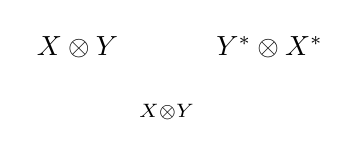
\begin{tikzpicture}[baseline={([yshift=-.5ex]current bounding box.center)}]
                \coordinate (A) at (0,0);
                \coordinate (B) at (1,0);
                \node[left] at (A) {$X \otimes Y$};
                \node[right] at (B) {$Y^* \otimes X^*$};
                \LCOEV{A}{B}
                \node[below] at (0.5,-0.6) {$\lcoev_{X \otimes Y}$};
            \end{tikzpicture}
            &\quad \coloneqq \quad 
            \begin{tikzpicture}[baseline={([yshift=-.5ex]current bounding box.center)}]
                \coordinate (A) at (0,0);
                \coordinate (B) at (1,0);
                \coordinate (C) at (2,0);
                \coordinate (D) at (3,0);
                \node[left] at (A) {$X$};
                \node[left] at (B) {$Y$};
                \node[right] at (C) {$Y^*$};
                \node[right] at (D) {$X^*$};
                \LCOEV{A}{D}
                \LCOEV{B}{C}
            \end{tikzpicture}, \\
            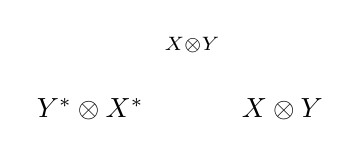
\begin{tikzpicture}[baseline={([yshift=-.5ex]current bounding box.center)}]
                \coordinate (A) at (0,0);
                \coordinate (B) at (1,0);
                \node[left] at (A) {$Y^* \otimes X^*$};
                \node[right] at (B) {$X \otimes Y$};
                \LEV{A}{B}
                \node[above] at (0.5,0.6) {$\lev_{X \otimes Y}$};
            \end{tikzpicture}
            &\quad \coloneqq \quad 
            \begin{tikzpicture}[baseline={([yshift=-.5ex]current bounding box.center)}]
                \coordinate (A) at (0,0);
                \coordinate (B) at (1,0);
                \coordinate (C) at (2,0);
                \coordinate (D) at (3,0);
                \node[left] at (A) {$X$};
                \node[left] at (B) {$Y$};
                \node[right] at (C) {$Y^*$};
                \node[right] at (D) {$X^*$};
                \LEV{A}{D}
                \LEV{B}{C}
            \end{tikzpicture}
        \end{align}
        なので明らか.
    \end{enumerate}
\end{proof}


全く同様にして,反変関手
\begin{align}
    \rdual{(\mhyphen)} \colon \Cat{C} \lto \Cat{C}
\end{align}
を作ることができる.

\begin{myexample}[label=def:dual-functor]{双対関手}
    補題\ref{lem:ldual-functor}より,\hyperref[redef:rigid]{rigidなモノイダル圏} $(\Cat{C},\, \otimes,\, I,\, a,\, l,\, r,\, \lev,\, \lcoev,\, \rev,\, \rcoev)$ において関手
    \begin{align}
        (\mhyphen)^{**} \colon \Cat{C} &\lto \Cat{C} \\
        {}^{**}(\mhyphen) \colon \Cat{C} &\lto \Cat{C}
    \end{align}
    は\hyperref[redef:monidal-functor]{厳密なモノイダル関手}である.
\end{myexample}


\begin{mylem}[label=lem:rigid-hom]{rigidity isomorphism}
    \hyperref[redef:rigid]{rigidなモノイダル圏} $(\Cat{C},\, \otimes,\, I,\, a,\, l,\, r,\, \lev,\, \lcoev,\, \rev,\, \rcoev)$ に対し,以下が成り立つ:
    \begin{enumerate}
        \item $\forall X,\, Y,\, Z \in \Obj{\Cat{C}}$ に対して\hyperref[def:nat]{自然な同型}
        \begin{align}
            \alpha_{X,Y,Z}\colon \Hom{\Cat{C}} (X \otimes Y,\, Z) &\xrightarrow{\cong} \Hom{\Cat{C}} (X,\, Z \otimes Y^*) \\
            \beta_{Y,X,Z}\colon \Hom{\Cat{C}} (Y^* \otimes X,\, Z) &\xrightarrow{\cong} \Hom{\Cat{C}} (X,\, Y \otimes Z)
        \end{align}
        が存在する.
        \item $\forall X,\, Y,\, Z \in \Obj{\Cat{C}}$ に対して\hyperref[def:nat]{自然な同型}
        \begin{align}
            \gamma_{X,Y,Z}\colon \Hom{\Cat{C}} (X \otimes \rdual{Y},\, Z) &\xrightarrow{\cong} \Hom{\Cat{C}} (X,\, Z \otimes Y) \\
            \gamma_{Y,X,Z}\colon \Hom{\Cat{C}} (Y \otimes X,\, Z) &\xrightarrow{\cong} \Hom{\Cat{C}} (X,\, \rdual{Y} \otimes Z)
        \end{align}
        が存在する.
    \end{enumerate}
    
\end{mylem}

\begin{proof}
    \begin{enumerate}
        \item 最初の同型は
        \begin{align}
            \alpha_{X,Y,Z} \colon 
                \begin{tikzpicture}[baseline={([yshift=-.5ex]current bounding box.center)}]
                    \path coordinate[label=left:$X$] (X)
                    ++(1,0) coordinate[label=right:$Y$] (Y)
                    ++(-0.5,1) coordinate[bullet,label=right:$f$] (f)
                    ++(0,1) coordinate[label=left:$Z$] (Z);
                    \draw[->-=.5] (X) -- (f);
                    \draw[->-=.5] (Y) -- (f);
                    \draw[->-=.5] (f) -- (Z);
                \end{tikzpicture}
                &\lmto 
                    \begin{tikzpicture}[baseline={([yshift=-.5ex]current bounding box.center)}]
                        \path coordinate[label=left:$X$] (X)
                        +(2,0) coordinate[label=right:$Y^*$] (W)
                        ++(1,0) coordinate[label=right:$Y$] (Y)
                        ++(-0.5,1) coordinate[bullet,label=right:$f$] (f)
                        ++(0,1) coordinate[label=left:$Z$] (Z);
                        \draw[->-=.5] (X) -- (f);
                        \draw[->-=.5] (Y) -- (f);
                        \draw[->-=.5] (f) -- (Z);
                        \draw[-<-=.5] (X) -- ++(0,-1);
                        \draw[-<-=.5] (W) -- ++(0,2);
                        \LCOEV{Y}{W}
                    \end{tikzpicture} \\
            \alpha_{X,Y,Z}^{-1} \colon 
            \begin{tikzpicture}[baseline={([yshift=-.5ex]current bounding box.center)}]
                \path coordinate[label=left:$X$] (X)
                ++(0,1) coordinate[bullet,label=right:$g$] (g)
                +(-0.5,1) coordinate[label=left:$Z$] (Z)
                +(0.5,1) coordinate[label=left:$Y^*$] (Y);
                \draw[->-=.5] (X) -- (g);
                \draw[->-=.5] (g) -- (Z);
                \draw[->-=.5] (Y) -- (g);
            \end{tikzpicture}
            &\lmto 
                \begin{tikzpicture}[baseline={([yshift=-.5ex]current bounding box.center)}]
                    \path coordinate[label=left:$X$] (X)
                    ++(0,1) coordinate[bullet,label=right:$g$] (g)
                    +(-0.5,1) coordinate[label=left:$Z$] (Z)
                    +(0.5,1) coordinate[label=left:$Y^*$] (Y)
                    ++(1.5,1) coordinate[label=left:$Y$] (W);
                    \draw[->-=.5] (X) -- (g);
                    \draw[->-=.5] (g) -- (Z);
                    \draw[->-=.5] (Y) -- (g);
                    \LEV{Y}{W}
                    \draw[-<-=.5] (W) -- ++(0,-2);
                \end{tikzpicture}
        \end{align}
        である.他も同様.
        \item (1) と同様.
    \end{enumerate}
    
\end{proof}

\subsection{組紐付きモノイダル圏}

\begin{mydef}[label=redef:braided-monoidal]{組紐付きモノイダル圏}
    \textbf{組紐付きモノイダル圏} (braided monoidal category) とは,以下の2つからなる:
    \begin{itemize}
        \item \hyperref[redef:monoidal-category]{モノイダル圏} $(\mathcal{C},\, \otimes,\, I,\, a,\, l,\, r)$
        \item \textbf{組紐} (braiding) と呼ばれる自然同型
        \begin{align}
            \Familyset[\big]{b_{X,\, Y} \colon X \otimes Y \xrightarrow{\cong} Y \otimes X}{X,\, Y \in \Obj{\mathcal{C}}}
        \end{align}
    \end{itemize}
    これらは $\forall X,\, Y,\, Z \in \Obj{\mathcal{C}}$ について以下の図式を可換にする:
    \begin{description}
        \item[\textbf{(hexagon diagrams)}] 
        
        \begin{center}
            \begin{tikzcd}[row sep=large, column sep=large]
                &X \otimes (Y \otimes Z) \ar[r, "a_{X,\, Y,\, Z}^{-1}"]\ar[d, "b_{X,\, Y \otimes Z}"] &(X \otimes Y) \otimes Z \ar[r, "b_{X,\, Y} \otimes \mathrm{Id}_Z"] &(Y \otimes X) \otimes Z \ar[d, "a_{Y,\, X,\, Z}"] \\
                &(Y \otimes Z) \otimes X &Y \otimes (Z \otimes X) \ar[l, "a_{Y,\, Z,\, X}^{-1}"] &Y \otimes (X \otimes Z) \ar[l, "\mathrm{Id}_Y \otimes b_{X,\, Z}"]
            \end{tikzcd}
        \end{center}
        
        \begin{center}
            \begin{tikzcd}[row sep=large, column sep=large]
                &(X \otimes Y) \otimes Z \ar[r, "a_{X,\, Y,\, Z}"]\ar[d, "b_{X \otimes Y ,\, Z}"] &X \otimes (Y \otimes Z) \ar[r, "\mathrm{Id}_X \otimes b_{Y,\, Z}"] &X \otimes (Z \otimes Y) \ar[d, "a_{X,\, Z,\, Y}^{-1}"] \\
                &Z \otimes (X \otimes Y) &(Z \otimes X) \otimes Y \ar[l, "a_{Z,\, X,\, Y}"] &(X \otimes Z) \otimes Y \ar[l, "b_{X,\, Z} \otimes \mathrm{Id}_Y"]
            \end{tikzcd}
        \end{center}
    \end{description}
    \tcblower
    組紐付きモノイダル圏 $\mathcal{C}$ であって,$\mathcal{C}$ の組紐が $b_{Y,\, X} \circ b_{X,\, Y} = \Id_{X \otimes Y}$ を充たすもののことを\textbf{対称モノイダル圏} (symmetric monoidal category) と呼ぶ.
\end{mydef}
ストリング図式で書く場合は
\begin{align}
    b_{X,\, Y} &\eqqcolon
    \begin{tikzpicture}[baseline={([yshift=-.5ex]current bounding box.center)}]
        \path coordinate[label=above left:$X$] (dx)
        +(1,0) coordinate[label=above right:$Y$] (dy)
        +(0,1) coordinate (uy)
        +(1,1) coordinate (ux);
        \BRAID{dx}{dy}{uy}{ux}
    \end{tikzpicture}
    &
    b^{-1}_{X,\, Y} &\eqqcolon
    \begin{tikzpicture}[baseline={([yshift=-.5ex]current bounding box.center)}]
        \path coordinate[label=above left:$X$] (dx)
        +(1,0) coordinate[label=above right:$Y$] (dy)
        +(0,1) coordinate (uy)
        +(1,1) coordinate (ux);
        \ABRAID{dx}{dy}{uy}{ux}
    \end{tikzpicture}
\end{align}
とする.\hyperref[redef:braided-monoidal]{\textsf{\textbf{(hexagon diagrams)}}}をストリング図式で表すと
\begin{align}
    \begin{tikzpicture}[baseline={([yshift=-.5ex]current bounding box.center)}]
        \path
        coordinate[label=above left:$X$] (x_2)
        +(1,0) coordinate[label=above right:$Y$] (y_2)
        +(3,0) coordinate[label=above right:$Z$] (z_2)
        ++(0,2) coordinate (y_3)
        +(1,0) coordinate (x_3)
        +(3,0) coordinate (z_3)
        ++(0,1) coordinate (y_4)
        +(2,0) coordinate (x_4)
        +(3,0) coordinate (z_4)
        ++(0,2) coordinate[label=below left:$Y$] (y_5)
        +(2,0) coordinate[label=below left:$Z$] (z_5)
        +(3,0) coordinate[label=below right:$X$] (x_5)
        ;
        % braiding
        \BRAID{x_2}{y_2}{y_3}{x_3}
        \draw[->-=.5] (z_2) -- (z_3);
        % associator
        \draw[->-=.5] (y_3) -- (y_4);
        \draw[->-=.5] (x_3) .. controls +(0,1) and +(0,-1) .. (x_4);
        \draw[->-=.5] (z_3) -- (z_4);
        % braiding
        \draw[->-=.5] (y_4) -- (y_5);
        \BRAID{x_4}{z_4}{z_5}{x_5}
    \end{tikzpicture}
    &\quad = \quad
    \begin{tikzpicture}[baseline={([yshift=-.5ex]current bounding box.center)}]
        \path 
        coordinate[label=above left:$X$] (x_2)
        +(1,0) coordinate[label=above right:$Y$] (y_2)
        +(3,0) coordinate[label=above right:$Z$] (z_2)
        ++(0,1) coordinate (x_3)
        +(2.7,0) coordinate (y_3)
        +(3,0) coordinate (z_3)
        ++(0,3) coordinate (y_4)
        +(0.3,0) coordinate (z_4)
        +(3,0) coordinate (x_4)
        ++(0,1) coordinate[label=below left:$Y$]  (y_5)
        +(2,0) coordinate[label=below left:$Z$] (z_5)
        +(3,0) coordinate[label=below right:$X$] (x_5)
        ;
        % associator
        \draw[->-=.5] (x_2) -- (x_3);
        \draw[->-=.5] (y_2) .. controls +(0,1) and +(0,-1) .. (y_3);
        \draw[->-=.5] (z_2) -- (z_3);
        % braiding
        \BRAID{x_3}{y_3}{y_4}{x_4}
        \BRAID{x_3}{z_3}{z_4}{x_4}
        % associator
        \draw[->-=.5] (y_4) -- (y_5);
        \draw[->-=.5] (z_4) .. controls +(0,1) and +(0,-1) .. (z_5);
        \draw[->-=.5] (x_4) -- (x_5);
    \end{tikzpicture}
\end{align}
および
\begin{align}
    \begin{tikzpicture}[baseline={([yshift=-.5ex]current bounding box.center)}]
        \path
        coordinate[label=above left:$X$] (x_2)
        +(2,0) coordinate[label=above right:$Y$] (y_2)
        +(3,0) coordinate[label=above right:$Z$] (z_2)
        ++(0,2) coordinate (x_3)
        +(2,0) coordinate (z_3)
        +(3,0) coordinate (y_3)
        ++(0,1) coordinate (x_4)
        +(1,0) coordinate (z_4)
        +(3,0) coordinate (y_4)
        ++(0,2) coordinate[label=below left:$Z$] (z_5)
        +(1,0) coordinate[label=below left:$X$] (x_5)
        +(3,0) coordinate[label=below right:$Y$] (y_5)
        ;
        % braiding
        \BRAID{y_2}{z_2}{z_3}{y_3}
        \draw[->-=.5] (x_2) -- (x_3);
        % associator
        \draw[->-=.5] (x_3) -- (x_4);
        \draw[->-=.5] (z_3) .. controls +(0,1) and +(0,-1) .. (z_4);
        \draw[->-=.5] (y_3) -- (y_4);
        % braiding
        \draw[->-=.5] (y_4) -- (y_5);
        \BRAID{x_4}{z_4}{z_5}{x_5}
    \end{tikzpicture}
    &\quad =  \quad 
    \begin{tikzpicture}[baseline={([yshift=-.5ex]current bounding box.center)}]
        \path 
        coordinate[label=above left:$X$] (x_2)
        +(2,0) coordinate[label=above right:$Y$] (y_2)
        +(3,0) coordinate[label=above right:$Z$] (z_2)
        ++(0,1) coordinate (x_3)
        +(0.3,0) coordinate (y_3)
        +(3,0) coordinate (z_3)
        ++(0,3) coordinate (z_4)
        +(2.7,0) coordinate (x_4)
        +(3,0) coordinate (y_4)
        ++(0,1) coordinate[label=below left:$Z$]  (z_5)
        +(1,0) coordinate[label=below left:$X$] (x_5)
        +(3,0) coordinate[label=below right:$Y$] (y_5)
        ;
        % associator
        \draw[->-=.5] (x_2) -- (x_3);
        \draw[->-=.5] (y_2) .. controls +(0,1) and +(0,-1) .. (y_3);
        \draw[->-=.5] (z_2) -- (z_3);
        % braiding
        \BRAID{x_3}{z_3}{z_4}{x_4}
        \BRAID{y_3}{z_3}{z_4}{y_4}
        % associator
        \draw[->-=.5] (z_4) -- (z_5);
        \draw[->-=.5] (x_4) .. controls +(0,1) and +(0,-1) .. (x_5);
        \draw[->-=.5] (y_4) -- (y_5);
    \end{tikzpicture}
\end{align}
のようになる.ただし,\hyperref[redef:monoidal-category]{associator}を明示的に描いた.この図式から,\hyperref[redef:braided-monoidal]{組紐}を含むストリング図式がアイソトピーに関して不変であることが分かる.

\hyperref[redef:braided-monoidal]{組紐付きモノイダル圏} $(\Cat{C},\, \otimes,\, I,\, a,\, l,\, r,\, b)$ が\hyperref[redef:braided-monoidal]{対称}であるとき,ストリング図式において
\begin{align}
    \begin{tikzpicture}[baseline={([yshift=-.5ex]current bounding box.center)}]
        \path 
            coordinate (x_1)
            +(1,0) coordinate (y_1)
            ++(0,1) coordinate (y_2)
            +(1,0) coordinate (x_2)
            ++(0,1) coordinate (x_3)
            +(1,0) coordinate (y_3)
        ;
        \BRAID{x_1}{y_1}{y_2}{x_2}
        \BRAID{y_2}{x_2}{x_3}{y_3}
    \end{tikzpicture}
    \quad &= \quad
    \begin{tikzpicture}[baseline={([yshift=-.5ex]current bounding box.center)}]
        \path coordinate (x)
        +(1,0) coordinate (y)
        ;
        \draw[->-=.5] (x) -- +(0,2);
        \draw[->-=.5] (y) -- +(0,2);
    \end{tikzpicture}
\end{align}
が成り立つ.

\begin{mydef}[label=def:braided-monoidal-functor]{組紐付きモノイダル関手}
    2つの\hyperref[redef:braided-monoidal]{組紐付きモノイダル圏} 
    $(\Cat{C},\, \otimes_{\Cat{C}},\, I_{\Cat{C}},\, a^{\Cat{C}},\, l^{\Cat{C}},\, r^{\Cat{C}},\, b^{\Cat{C}}),\, (\Cat{D},\, \otimes_{\Cat{D}},\, I_{\Cat{D}},\, a^{\Cat{D}},\, l^{\Cat{D}},\, r^{\Cat{D}},\, b^{\Cat{D}})$ の間の\hyperref[def:monidal-functor]{弱いモノイダル関手}
    $(F \colon \Cat{C} \lto \Cat{D},\; \varepsilon,\, \mu)$ が\textbf{弱い組紐付きモノイダル関手} (lax braided monoidal functor) であるとは,
    $\forall X,\, Y \in \Obj{\Cat{C}}$ に対して以下の図式が可換になること:

    \begin{center}
        \begin{tikzcd}[row sep=large, column sep=large]
            &F(X) \otimes_{\Cat{D}} F(Y) \ar[d, "\mu_{X,\, Y}"']\ar[rr, "b^{\Cat{D}}_{F(X),F(Y)}"] & &F(Y)\otimes_{\Cat{D}} F(X) \ar[d, "\mu_{Y,\, X}"] \\
            &F(X \otimes_{\Cat{C}} Y) \ar[rr, "F(b^{\Cat{C}}_{X,\, Y})"] & &F(Y \otimes_{\Cat{C}}X)
        \end{tikzcd}
    \end{center}
\end{mydef}

\begin{myprop}[label=prop:YBeq]{Yang-Baxter方程式}
    \hyperref[redef:braided-monoidal]{組紐付きモノイダル圏} $(\Cat{C},\, I,\, a,\, l,\, r,\, b)$ を与える.
    このとき,$\forall X,\, Y,\, Z \in \Obj{\Cat{C}}$ に対して以下が成り立つ:
    \begin{align}
        &a_{Y,\, Z,\, X} \circ (b_{Y,\, Z} \otimes \Id_X) \circ a_{Y,\, Z,\, X}^{-1} \circ (\Id_Y \otimes b_{X,\, Z}) \circ a_{Y,\, X,\, Z} \circ (b_{X,\, Y} \otimes \Id_Z) \\
        &= (\Id_{Z} \otimes b_{X,\, Y}) \circ a_{Z,\, X,\, Y} \circ (b_{X,\, Z} \otimes \Id_{Y}) \circ a_{X,\, Z,\, Y}^{-1} \circ (\Id_{X} \otimes b_{Y,\, Z}) \circ a_{X,\, Y,\, Z}
    \end{align}
\end{myprop}

\begin{proof}
    圏 $\Cat{C}$ における図式
    \begin{center}
        \begin{tikzcd}[column sep=large]
            % 行1:7セル(最初と最後は空セル)
            &X \otimes (Y \otimes Z) \ar[d, red, "\Id_X \otimes b_{Y,Z}"'] 
              & (X \otimes Y) \otimes Z \ar[l, red, "\cong"'] \ar[ddd, "b_{(X \otimes Y),Z}"] \ar[r, "b_{X,Y} \otimes \Id_{Z}"] 
              & (Y \otimes X) \otimes Z \ar[ddd, "b_{(Y \otimes X),Z}"] \ar[r, red, "\cong"] 
              & Y \otimes (X \otimes Z) \ar[d, red, "\Id_X \otimes b_{X,Z}"] 
            \\
            % 行2:7セル(1列目、7列目が空)
            &X \otimes (Z \otimes Y) \ar[d, red, "\cong"'] 
             & &
            &Y \otimes (Z \otimes X) \ar[d, red, "\cong"] 
            \\
            % 行3:7セル(2,3,4,6,7列目が空)
            &(X \otimes Z) \otimes Y \ar[d, red, "b_{X,Z} \otimes \Id_Y"'] 
              & &
            &(Y \otimes Z) \otimes X \ar[d, red, "b_{Y,Z} \otimes \Id_X"] 
            \\
            % 行4:7セル(1,2,6,7列目が空)
            &(Z \otimes X) \otimes Y \ar[r, red, "\cong"'] 
              & Z \otimes (X \otimes Y) \ar[r, "\Id_Z \otimes b_{X, Y}"']
              & Z \otimes (Y \otimes X)
              & (Z \otimes Y) \otimes X \ar[l, red, "\cong"] 
          \end{tikzcd}
        % \begin{tikzcd}
        %     & &X \otimes (Y \otimes Z) \ar[dl, red, "\Id_X \otimes b_{Y,Z}"'] &(X \otimes Y) \otimes Z \ar[l,red,"\cong"']\ar[ddd, "b_{(X \otimes Y),Z}"]\ar[r, "b_{X,Y} \otimes \Id_{Z}"] &(Y \otimes X) \otimes Z \ar[ddd,"b_{(Y \otimes X),Z}"] \ar[r,red, "\cong"] &Y \otimes (X \otimes Z) \ar[dr,red, "\Id_X \otimes b_{X,Z}"] & \\
        %     &X \otimes (Z \otimes Y) \ar[d, red, "\cong"'] & & & &Y \otimes (Z \otimes X) \ar[d,red,"\cong"] \\
        %     &(X \otimes Z) \otimes Y \ar[dr, red, "b_{X,\, Z} \otimes \Id_Y"'] & & & &(Y \otimes Z) \otimes X \ar[dl,red,"b_{Y,Z} \otimes \Id_X"] \\
        %     & &Z \otimes (X \otimes Y) \ar[r,red,"\cong"'] &(Y \otimes Z) \otimes X &(Z \otimes Y) \otimes X \ar[l,red,"\cong"] &
        % \end{tikzcd}
    \end{center}
    を考える.ただし $\cong$ はassociatorを表す.
    赤色の部分は\hyperref[redef:braided-monoidal]{\textsf{\textbf{(hexagon diagrams)}}}そのものなので可換である.
    また,中央の四角形は $b$ が\hyperref[def:nat]{自然変換}であることから可換である.
    故に図式の外周部は可換であり,示された.
\end{proof}

\begin{marker}
    以降,原則としてストリング図式においては\hyperref[redef:monoidal-category]{associator}を描画しない.
\end{marker}

命題\ref{prop:YBeq}をストリング図式で書くと次のようになる:

\begin{align}
    \label{eq:YB}
    \begin{tikzpicture}[baseline={([yshift=-.5ex]current bounding box.center)}]
        \path 
            coordinate (O)
            foreach \i in {1,...,4} {
                ++(0,1) coordinate (x_\i)
                +(1,0) coordinate (y_\i)
                +(2,0) coordinate (z_\i)
            }
        ;
        \node[above left] at (x_1) {$X$};
        \node[above right] at (y_1) {$Y$};
        \node[above right] at (z_1) {$Z$};
        \node[above left] at (x_4) {$Z$};
        \node[above right] at (y_4) {$Y$};
        \node[above right] at (z_4) {$X$};
        \BRAID{x_1}{y_1}{x_2}{y_2}
        \BRAID{y_2}{z_2}{y_3}{z_3}
        \BRAID{x_3}{y_3}{x_4}{y_4}
        \draw[->-=.5] (z_1) -- (z_2);
        \draw[->-=.5] (x_2) -- (x_3);
        \draw[->-=.5] (z_3) -- (z_4);
    \end{tikzpicture}
    \quad &=\quad 
    \begin{tikzpicture}[baseline={([yshift=-.5ex]current bounding box.center)}]
        \path 
            coordinate (O)
            foreach \i in {1,...,4} {
                ++(0,1) coordinate (x_\i)
                +(1,0) coordinate (y_\i)
                +(2,0) coordinate (z_\i)
            }
        ;
        \node[above left] at (x_1) {$X$};
        \node[above right] at (y_1) {$Y$};
        \node[above right] at (z_1) {$Z$};
        \node[above left] at (x_4) {$Z$};
        \node[above right] at (y_4) {$Y$};
        \node[above right] at (z_4) {$X$};
        \BRAID{y_1}{z_1}{y_2}{z_2}
        \BRAID{x_2}{y_2}{x_3}{y_3}
        \BRAID{y_3}{z_3}{y_4}{z_4}
        \draw[->-=.5] (x_1) -- (x_2);
        \draw[->-=.5] (z_2) -- (z_3);
        \draw[->-=.5] (x_3) -- (x_4);
    \end{tikzpicture}
\end{align}

\begin{mylem}[label=lem:dual-braid]{dualと組紐}
    \hyperref[redef:braided-monoidal]{組紐}付き\hyperref[redef:rigid]{rigidモノイダル圏} $(\Cat{C},\, \otimes,\, I,\, a,\, l,\, r,\, \lev,\, \lcoev,\, \rev,\, \rcoev,\, b)$ を与える.
    このとき,$\forall X,\, Y \in \Obj{\Cat{C}}$ に対して以下が成り立つ:
    \begin{enumerate}
        \item 
        \begin{align}
            l_X \circ b_{X,\, I} &= r_X, 
            &
            r_X \circ b_{I,\, X} &= l_X, 
            &
            b_{I,\, X} \circ b_{X,\, I} &= \Id_{X \otimes I}
        \end{align}
        \item 
        \begin{align}
            (\lcoev_X \otimes \Id_Y) \circ l_Y^{-1} = b_{Y,\, X \otimes X^*} \circ (\Id_y \otimes \lcoev_X) \circ r_Y^{-1}
        \end{align}
        \item 
        \begin{align}
            r_Y \circ (\Id_Y \otimes \lev_X)  = l_Y \circ (\lev_X \otimes \Id_Y) \circ b_{Y,\, X^* \otimes X}
        \end{align}
    \end{enumerate}
\end{mylem}

\begin{proof}
    \begin{enumerate}
        \item ~\cite[EXERCISE 8.1.6, p.196]{etingof2015tensor}
        % \hyperref[redef:braided-monoidal]{\textsf{\textbf{(hexagon diagrams)}}}において $Y=Z=I$ と選ぶことで,
        % \begin{align}
        %     b_{X,\, I\otimes I} \circ a_{X,I,I} &= a_{I,I,X}^{-1} \circ (\Id_I \otimes b_{X,\, I}) \circ a_{I,X,I} \circ (b_{X,\, I} \otimes \Id_I)
        % \end{align}
        % が分かる.命題\ref{prop:monidal-unit}-(3), (4) より
        % \begin{align}
        %     a_{X,I,I} = (r_X \otimes \Id) \circ (\Id_X \otimes l_I^{-1}),\quad a_{I,I,X}^{-1} = (l_I^{-1} \otimes \Id_I) \circ (\Id_I \otimes l_X)
        % \end{align}
        % が成り立つので
        \item 以下の図式を考える:
        \begin{center}
            \begin{tikzcd}[row sep=large, column sep=large]
                 & &I \otimes Y \ar[r, "\lcoev_X \otimes \Id_Y"] &(X \otimes X^*) \otimes Y \\
                 &Y \ar[ur, "l_Y^{-1}"]\ar[dr, "r_Y^{-1}"']&                 & \\
                 & &Y \otimes I \ar[r, "\Id_Y \otimes \lcoev_X"']\ar[uu, "b_{Y,I}"'] &Y \otimes (X \otimes X^*) \ar[uu, "b_{Y,X \otimes X^*}"']
            \end{tikzcd}
        \end{center}
        左端の三角形は (1) より可換である.
        四角形は,圏 $\Cat{C} \otimes \Cat{C}$ における射 $(\Id_Y,\, \lcoev_X)$ に対して $b \colon \otimes \Longrightarrow \otimes \circ \tau$ の自然性を用いることで可換だとわかる.
        よって外周部も可換であり,示された.
        \item (1) と同様.
    \end{enumerate}
\end{proof}

補題\ref{lem:dual-braid}-(2), (3) をストリング図式で書くと次のようになる:
\begin{align}
    \begin{tikzpicture}[baseline={([yshift=-.5ex]current bounding box.center)}]
        \path coordinate (y_1)
            ++(0,3) coordinate[label=below right:$Y$] (y_2)
            ++(-1,0) coordinate[label=below right:$X^*$] (x_2)
            ++(-1,0) coordinate[label=below left:$X$] (x_1)
        ;
        \LCOEV{x_1}{x_2}
        \draw[->-=.5] (y_1) -- (y_2);
    \end{tikzpicture}
    &\quad = \quad
    \begin{tikzpicture}[baseline={([yshift=-.5ex]current bounding box.center)}]
        \path coordinate (y_1)
            ++(0,1) coordinate(y_2)
            +(2,0) coordinate(x_1)
            +(3,0) coordinate (x_2)
            ++(0,2)coordinate[label=below left:$X$]  (x_3)
            +(1,0) coordinate[label=below right:$X^*$]  (x_4)
            +(3,0) coordinate[label=below right:$Y$] (y_3)
        ;
        \draw[->-=.5] (y_1) -- (y_2);
        \LCOEV{x_1}{x_2}
        \BRAID{y_2}{x_1}{x_3}{y_3}
        \BRAID{y_2}{x_2}{x_4}{y_3}
    \end{tikzpicture} \\
    \begin{tikzpicture}[baseline={([yshift=-.5ex]current bounding box.center)}]
        \path coordinate (y_1)
        ++(0,3) coordinate (y_2)
        +(1,0) coordinate (x_2)
        +(2,0) coordinate (z_2)
        ;
        \draw[->-=.5] (y_1) -- (y_2);
        \LCOEV{x_2}{z_2}
    \end{tikzpicture}
    &\quad = \quad
    \begin{tikzpicture}[baseline={([yshift=-.5ex]current bounding box.center)}]
        \path coordinate (x_1)
        +(1,0) coordinate (y_1)
        + (3,0) coordinate (z_1)
        ++(0,2) coordinate (x_2)
        +(2,0) coordinate (y_2)
        +(3,0) coordinate (z_2)
        ;
        \LCOEV{x_1}{y_1}
        \draw[-<-=.5] (z_1) -- +(0,-1);
        \ABRAID{x_1}{z_1}{x_2}{y_2}
        \ABRAID{y_1}{z_1}{x_2}{z_2}
    \end{tikzpicture} \\
    \begin{tikzpicture}[baseline={([yshift=-.5ex]current bounding box.center)}]
        \path coordinate[label=above left:$Y$] (y_1)
            +(1,0) coordinate[label=above left:$X^*$] (x_1)
            +(2,0) coordinate[label=above right:$X$] (x_2)
            ++(0,3) coordinate (y_2)
        ;
        \draw[->-=.5] (y_1) -- (y_2);
        \LEV{x_1}{x_2}
    \end{tikzpicture}
    &\quad = \quad
    \begin{tikzpicture}[baseline={([yshift=-.5ex]current bounding box.center)}]
        \path coordinate[label=above left:$Y$] (x_1)
            +(2,0) coordinate[label=above left:$X^*$] (y_1)
            +(3,0) coordinate[label=above right:$X$] (z_1)
            ++(0,2) coordinate (x_2)
            +(1,0) coordinate (y_2)
            +(3,0) coordinate (z_2)
        ;
        \BRAID{x_1}{y_1}{x_2}{z_2}
        \BRAID{x_1}{z_1}{y_2}{z_2}
        \LEV{x_2}{y_2}
        \draw[->-=.5] (z_2) -- +(0,1);
    \end{tikzpicture} \\
    \begin{tikzpicture}[baseline={([yshift=-.5ex]current bounding box.center)}]
        \path coordinate (x_1)
        +(1,0) coordinate (y_1)
        +(2,0) coordinate (z_1)
        ++(2,3) coordinate (z_2)
        ;
        \LEV{x_1}{y_1}
        \draw[->-=.5] (z_1) -- (z_2);
    \end{tikzpicture}
    &\quad = \quad
    \begin{tikzpicture}[baseline={([yshift=-.5ex]current bounding box.center)}]
        \path coordinate (x_1)
        +(1,0) coordinate (y_1)
        +(3,0) coordinate (z_1)
        ++(0,2) coordinate (x_2)
        +(2,0) coordinate (y_2)
        +(3,0) coordinate (z_2)
        ;
        \LEV{y_2}{z_2}
        \draw[->-=.5] (x_2) -- +(0,1);
        \ABRAID{x_1}{z_1}{x_2}{y_2}
        \ABRAID{y_1}{z_1}{x_2}{z_2}
    \end{tikzpicture}
\end{align}
ただし\hyperref[redef:monoidal-category]{left/right unitor}を省略した.
つまり,端で折り返している組紐は,下を潜らせることができる.

\subsection{リボン構造}

\begin{mydef}[label=def:ribbon]{リボン構造}
    \hyperref[redef:braided-monoidal]{組紐}付き\hyperref[redef:rigid]{rigidモノイダル圏} $(\Cat{C},\, \otimes,\, 1,\, a,\, l,\, r,\, \lev,\, \lcoev,\, \rev,\, \rcoev,\, b)$ の
    \textbf{リボン構造} (ribbon structure) とは,
    \hyperref[def:nat]{自然同型} $\theta \colon \Id_{\Cat{C}} \Longrightarrow \Id_{\Cat{C}}$ であって以下を充たすもののこと:
    \begin{description}
        \item[\textbf{(Rib-1)}] $\forall X,\, Y \in \Obj{\Cat{C}}$ に対して $\theta_{X \otimes Y} = (\theta_{X} \otimes \theta_{Y}) \circ b_{Y,\, X} \circ b_{X,\, Y}$ が成り立つ.
        \item[\textbf{(Rib-2)}] $\forall X \in \Obj{\Cat{C}}$ に対して $(\theta_X)^* = \theta_{X^*}$
    \end{description}
\end{mydef}

ストリング図式で \textsf{\textbf{(Rib-1)}} を書くと
\begin{align}
    \begin{tikzpicture}[baseline={([yshift=-.5ex]current bounding box.center)}]
        \path coordinate (x_1)
            +(1,0) coordinate (y_1)
            ++(0.5,2) coordinate (q)
            ++(-0.5,2) coordinate (x_2)
            +(1,0) coordinate (y_2)
        ;
        \draw[->-=.2,->-=.8] (x_1) to[out=90,in=-120] node[midway,below left] {$X$} (q.center) to[out=120,in=-90] node[midway,above left]{$X$} (x_2);
        \draw[->-=.2,->-=.8] (y_1) to[out=90,in=-60] node[midway,below right] {$Y$} (q.center) to[out=60,in=-90] node[midway,above right] {$Y$} (y_2);
        \node[circlenode] at (q) {$\theta_{X \otimes Y}$};
    \end{tikzpicture}
    \quad &= \quad 
    \begin{tikzpicture}[baseline={([yshift=-.5ex]current bounding box.center)}]
        \path 
            coordinate (O)
            foreach \i in {1,...,5} {
                ++(0,1) coordinate (x_\i)
                +(1,0) coordinate (y_\i)
            }
        ;
        \BRAID{x_1}{y_1}{x_2}{y_2}
        \BRAID{x_2}{y_2}{x_3}{y_3}
        \draw[->-=.2,->-=.8] (x_3) -- (x_4) -- (x_5);
        \draw[->-=.2,->-=.8] (y_3) -- (y_4) -- (y_5);
        \node[circlenode,fill=white] at (x_4) {$\theta_X$};
        \node[circlenode,fill=white] at (y_4) {$\theta_Y$};
    \end{tikzpicture}
\end{align}
となり,\textsf{\textbf{(Rib-2)}} は
\begin{align}
    \begin{tikzpicture}[baseline={([yshift=-.5ex]current bounding box.center)}]
        \path coordinate (x_1)
            ++(1,0) coordinate (x_2)
            ++(0,-1) coordinate (q)
            ++(0,-1) coordinate (x_3)
            ++(1,0) coordinate (x_4)
        ;
        \LEV{x_1}{x_2}
        \LCOEV{x_3}{x_4}
        \draw[->-=.5] (x_1) -- +(0,-3);
        \draw[-<-=.5] (x_4) -- +(0,3);
        \draw[->-=.2,->-=.8] (x_3) -- (x_2);
        \node[circlenode] at (q) {$\theta_X$};
    \end{tikzpicture}
    \quad &= \quad
    \begin{tikzpicture}[baseline={([yshift=-.5ex]current bounding box.center)}]
        \path coordinate (x_1)
            ++(0,1.5) coordinate (q)
            ++(0,1.5) coordinate (x_2)
        ;
        \draw[->-=.2,->-=.8] (x_2) -- (q) -- (x_1);
        \node[circlenode] at (q) {$\theta_{X^*}$};
    \end{tikzpicture}
\end{align}
となる.



\section{テンソル圏・フュージョン圏}

\begin{marker}
    これまでは\hyperref[redef:monoidal-category]{モノイダル圏}の対象を英大文字 $X,\, Y,\, Z,\, \dots$ で,単位対象を $I$ と書いてきたが,以下では対象を英小文字 $x,\, y,\, z,\, \dots$ で,単位対象を $1$ と書くことにする.
\end{marker}

\begin{mydef}[label=def:ringcat]{環圏}
    圏 $\Cat{C}$ が\textbf{多重環圏} (multiring category) であるとは,以下の条件を充たすこと:
    \begin{description}
        \item[\textbf{(mR-1)}] $\Cat{C}$ は\hyperref[def:finite-abcat]{局所有限}な\hyperref[def:additive-cat]{$\mathbb{K}$-線形アーベル圏}
        \item[\textbf{(mR-2)}] $\Cat{C}$ は\hyperref[redef:rigid]{モノイダル圏} $(\Cat{C},\, \otimes,\, 1,\, a,\, l,\, r)$
        \item[\textbf{(mR-3)}] 関手 $\otimes \colon \Cat{C} \times \Cat{C} \lto \Cat{C}$ が $\mathbb{K}$-双線形かつ双完全
    \end{description}
    圏 $\Cat{C}$ が\textbf{環圏} (ring category) であるとは,以下の条件を充たすこと:
    \begin{description}
        \item[\textbf{(R-1)}] $\Cat{C}$ は多重環圏
        \item[\textbf{(R-2)}] $\Hom{\Cat{C}} (1,\, 1) \cong \mathbb{K}$ 
    \end{description}
\end{mydef}

\begin{mylem}[label=lem:1-simple-ringcat]{環圏における $1$ の単純性}
    \begin{enumerate}
        \item \hyperref[redef:dual]{左双対}を持つ\hyperref[def:ringcat]{多重環圏} $(\Cat{C},\, \otimes,\, 1,\, a,\, l,\, r,\, \lcoev,\, \lev)$ において,\hyperref[lem:ldual-functor]{左双対関手} $(\mhyphen)^* \colon \Cat{C} \lto \Cat{C}$ は\hyperref[def:additive-exact]{完全}である.
        \item \hyperref[redef:dual]{左双対}を持つ\hyperref[def:ringcat]{環圏} $(\Cat{C},\, \otimes,\, 1,\, a,\, l,\, r,\, \lcoev,\, \lev)$ において,$1 \in \Obj{\Cat{C}}$ は\hyperref[def:semisimple-cat]{単純対象}である.
    \end{enumerate}
\end{mylem}

\begin{proof}
    \begin{enumerate}
        \item 完全列 $0 \lto x \xrightarrow{f} y \xrightarrow{g} z \lto 0$ を与える.示すべきは $0 \lto z^* \xrightarrow{g^*} y^* \xrightarrow{f^*} x^* \lto 0$ が完全であることである.
        $\forall w \in \Obj{\Cat{C}}$ を1つとり,圏 $\Cat{C}$ における図式
        \begin{align}
            0 \lto \Hom{\Cat{C}}(w,\, z^*) \xrightarrow{\Hom{\Cat{C}}(w,\, g^*)} \Hom{\Cat{C}}(w,\, y^*) \xrightarrow{\Hom{\Cat{C}}(w,\, f^*)} \Hom{\Cat{C}}(w,\, x^*)
        \end{align}
        を考える.補題\ref{lem:rigid-hom}-(1) の自然同型によりこれは
        \begin{align}
            0 \lto \Hom{\Cat{C}}(w \otimes z,\, 1) \lto \Hom{\Cat{C}}(w \otimes y,\, 1) \lto \Hom{\Cat{C}}(w \otimes x,\, 1)
        \end{align}
        と書けるが,\hyperref[def:ringcat]{多重環圏の定義}より $\otimes$ は完全で,かつ $\Hom{\Cat{C}}(\mhyphen,\, 1)$ は左完全関手なので,これは完全列である.よって $0 \lto z^* \xrightarrow{g^*} y^* \xrightarrow{f^*} x^*$ は完全である.
        同様の議論から $z^* \xrightarrow{g^*} y^* \xrightarrow{f^*} x^* \lto 0$ の完全性も従う.

        \item 任意のゼロでない単純な部分対象 $x \overset{i}{\hookrightarrow} 1$ を1つとる\footnote{アーベル圏 $\Cat{C}$ の\hyperref[def:finite-abcat]{有限性}から,このような $x$ は存在する.}.
        $\Cat{C}$ は\hyperref[def:additivecat]{アーベル圏}なので $i$ の余核が存在し,
        \begin{align}
            0 \lto x \overset{i}{\hookrightarrow} 1 \xrightarrow{\coker i} \Coker i \lto 0
        \end{align}
        は完全列になる.(1) より
        \begin{align}
            0 \lto (\Coker i)^* \lto 1 \lto x^* \lto 0
        \end{align}
        は完全列である.さらに,\hyperref[def:ringcat]{環圏の定義}より $\otimes$ は完全なので
        \begin{align}
            \label{eq:1-simple-ringcat}
            0 \lto x \otimes (\Coker i)^* \lto x \lto x \otimes x^* \lto 0
        \end{align}
        も完全列だが,$x$ は単純でかつ $x \otimes x^* \neq 0$(evaluationが零射でないため)なので\footnote{\eqref{eq:1-simple-ringcat}は完全列なので $x \otimes (\Coker i)^* \lto x$ はモノ射であり,かつ $x \neq 0$ なので $\Coker i \neq 1$ であるから,$x \otimes (\Coker i)^* = 0$ が言える.} $x \otimes x^* \cong x$ が分かった.よってエピ射 $1 \xrightarrow{\lcoev_x} x \otimes x^* \lto x$ を得る.
        よって零射でない $1 \twoheadrightarrow x \overset{i}{\hookrightarrow} 1$ を得るが,$\Hom{\Cat{C}}(1,\, 1) = \mathbb{K}$ なので $x = 1$ でなくてはいけない.
    \end{enumerate}
\end{proof}

\begin{mydef}[label=def:tensorfusion-cat]{テンソル圏・フュージョン圏}
    圏 $\Cat{C}$ が\textbf{多重テンソル圏} (multitensor category) であるとは,以下の条件を充たすこと:
    \begin{description}
        \item[\textbf{(mT-1)}] $\Cat{C}$ は\hyperref[def:finite-abcat]{局所有限}な\hyperref[def:additive-cat]{$\mathbb{K}$-線形アーベル圏}
        \item[\textbf{(mT-2)}] $\Cat{C}$ は\hyperref[redef:rigid]{rigidなモノイダル圏} $(\Cat{C},\, \otimes,\, 1,\, a,\, l,\, r,\, \lev,\, \lcoev,\, \rev,\, \rcoev)$
        \item[\textbf{(mT-3)}] 関手 $\otimes \colon \Cat{C} \times \Cat{C} \lto \Cat{C}$ が $\forall x,\,y,\,z,\,w \in \Obj{\Cat{C}}$ に対して定める写像 $\otimes_{x,y,z,w} \colon \Hom{\Cat{C}} (x,\, y) \times \Hom{\Cat{C}} (z,\, w) \lto \Hom{\Cat{C}} (x \otimes z,\,  y \otimes w)$ が $\mathbb{K}$-双線形
    \end{description}
    圏 $\Cat{C}$ が\textbf{テンソル圏} (tensor category) であるとは,以下の条件を充たすこと:
    \begin{description}
        \item[\textbf{(T-1)}] $\Cat{C}$ は多重テンソル圏
        \item[\textbf{(T-2)}] $\Hom{\Cat{C}} (1,\, 1) \cong \mathbb{K}$ 
    \end{description}
    
    \tcblower

    圏 $\Cat{C}$ が\textbf{多重フュージョン圏} (multifusion category) であるとは,以下の条件を充たすこと:
    \begin{description}
        \item[\textbf{(mFus-1)}] $\Cat{C}$ は多重テンソル圏
        \item[\textbf{(mFus-2)}] $\Cat{C}$ は\hyperref[def:additive-cat]{$\mathbb{K}$-線形アーベル圏}として\hyperref[def:finite-abcat]{有限}かつ\hyperref[def:finite-abcat]{半単純}
    \end{description}
    圏 $\Cat{C}$ が\textbf{フュージョン圏} (fusion category) であるとは,以下の条件を充たすこと:
    \begin{description}
        \item[\textbf{(Fus-1)}] $\Cat{C}$ はテンソル圏
        \item[\textbf{(Fus-2)}] $\Cat{C}$ は\hyperref[def:additive-cat]{$\mathbb{K}$-線形アーベル圏}として\hyperref[def:finite-abcat]{有限}かつ\hyperref[def:finite-abcat]{半単純}
    \end{description}
\end{mydef}

\begin{myprop}[label=prop:tensor-ring]{多重テンソル圏のテンソル積は双完全}
    \hyperref[def:tensorfusion-cat]{多重テンソル圏} $\Cat{C}$ の関手 $\otimes \colon \Cat{C} \times \Cat{C} \lto \Cat{C}$ は双完全である.
\end{myprop}

\begin{proof}
    ~\cite[PROPOSITION 4.2.1., p.66]{etingof2015tensor}
\end{proof}

命題\ref{prop:tensor-ring}より,
\begin{align}
    \text{\hyperref[def:tensorfusion-cat]{(多重)テンソル圏}} \IMP \text{\hyperref[def:ringcat]{(多重)環圏}}
\end{align}
が言える.

\begin{myprop}[label=prop:1-simple]{テンソル圏における $1$ の単純性}
    \hyperref[def:tensorfusion-cat]{テンソル圏}において $1$ は\hyperref[def:semisimple-cat]{単純}である.
\end{myprop}

\begin{proof}
    命題\ref{prop:tensor-ring}と補題\ref{lem:1-simple-ringcat}と\hyperref[def:tensorfusion-cat]{テンソル圏の定義}から従う.
\end{proof}



\begin{myexample}[label=def:CG]{圏 $\Cat{C}_G$ と $\VecG{G}$}
    $G$ を群とする.\hyperref[redef:monoidal-category]{厳密なモノイダル圏} $\Cat{C}_G$ を,
    \begin{itemize}
        \item $\Obj{\Cat{C}_G} \coloneqq G$
        \item $\forall g_1,\, g_2 \in G$ に対して
        \begin{align}
            \Hom{\Cat{C}_G}(g_1,\, g_2) \coloneqq 
            \begin{cases}
                \LU(1), &g_1 = g_2 \\
                \emptyset, &g_1 \neq g_2
            \end{cases}
        \end{align}
        \item $g_1 \otimes g_2 \coloneqq g_1 g_2$ かつ,$g_i \xrightarrow{\forall \theta_i}  g_i$ に対して $\theta_1 \otimes \theta_2 \coloneqq \theta_1 \theta_2$
        \item $1 \coloneqq 1_G$
        \item $a_{g_1,g_2,g_3} \coloneqq 1,\; l_{g} \coloneqq 1,\, r_g \coloneqq 1$
    \end{itemize}
    で定義する.
    
    $\mathbb{K} = \mathbb{C}$ とする.\hyperref[redef:monoidal-category]{厳密なモノイダル圏} $\VecG{G}$ を,
    \begin{itemize}
        \item $G$-gradedな $\mathbb{K}$-ベクトル空間
        \begin{align}
            V = \bigoplus_{g \in G} V_g
        \end{align}
        を対象とする.
        \item gradingを保存する $\mathbb{K}$-線型変換
        \begin{align}
            f \colon \bigoplus_{g \in G} V_g \lto \bigoplus_{g \in G} W_g \quad \mathrm{s.t.} \quad \forall g \in G,\; f (V_g) \subset W_g
        \end{align}
        を射とする.
        \item テンソル積 $\otimes \colon \VecG{G} \times \VecG{G} \lto \VecG{G}$ は,
        \begin{align}
            V \otimes W \coloneqq \bigoplus_{g \in G} \left( \bigoplus_{\substack{x,\, y \in G, \\ xy = g}} V_x \otimes_{\mathbb{K}} W_y\right)
        \end{align}
        と定義する.
        \item 単位対象は $1 \coloneqq \mathbb{K}$ とする\footnote{$1_G \in G$ 成分以外が全て $0$}
        \item $a_{g_1,g_2,g_3} \coloneqq 1,\; l_{g} \coloneqq 1,\, r_g \coloneqq 1$
    \end{itemize}
    によって定義する.\underline{$G$ が有限群ならば} $\Cat{C}_G$ は\hyperref[def:tensorfusion-cat]{フュージョン圏}である.
\end{myexample}

\begin{myexample}[label=def:CGa]{圏 $\Cat{C}_G^\alpha$ と $\mathrm{Vec}^\alpha_G$}
    $G$ を群とする.\exref{def:CG}の\hyperref[redef:monoidal-category]{associatorとunitors}を非自明にしてみよう.
    今 $\alpha \in \irm{Z}{Grp}^3 \bigl(G;\, \LU(1)\bigr)$ を1つ固定する\footnote{i.e. 3-コサイクル}.
    
    \hyperref[redef:monoidal-category]{モノイダル圏} $\Cat{C}_G^\alpha$ を,
    \begin{align}
        a_{g_1,g_2,g_3} &\coloneqq \alpha(g_1,\, g_2,\, g_3), \\
        l_{g} &\coloneqq \alpha(1,\, 1,\, g)^{-1}, \\
        r_{g} &\coloneqq \alpha(g,\, 1,\, 1)
    \end{align}
    とおくことにより定義する\footnote{他のデータは\exref{def:CG}と全く同じである}.実際,コサイクル条件および $\LU(1)$ の可換性により
    \begin{align}
        &(\Id_{g_4} \otimes a_{g_1,g_2,g_3}) \circ a_{g_4,g_1 \otimes g_2,g_3} \circ (a_{g_4,g_1,g_2} \otimes \Id_{g_3}) \\
        &= \alpha(g_1,\, g_2,\, g_3) \alpha(g_4,\, g_1g_2,\, g_3) \alpha (g_4,\, g_1,\, g_2) \\
        &= \alpha(g_4g_1,\, g_2,\, g_3) \alpha(g_4,\, g_1,\, g_2g_3) \\
        &= \alpha(g_4,\, g_1,\, g_2g_3)\alpha(g_4g_1,\, g_2,\, g_3) \\
        &= a_{g_4,g_1,g_2g_3} \circ a_{g_4 \otimes g_1,\, g_2,\, g_3}
    \end{align}
    の通りに\hyperref[redef:monoidal-category]{\textsf{\textbf{(pentagon identity)}}}が成り立ち,
    \begin{align}
        (\Id_{g_1} \otimes l_{g_2}) \circ a_{g_1,1,g_2} 
        &= \frac{\alpha(g_1,\, 1,\, g_2)}{\alpha(1,\, 1,\, g_2)} \\
        &= \frac{\alpha(g_1,\, 1,\, 1)\cancel{\alpha(g_1,\, 1,\, g_2)\alpha(1,\,1,\, g_2)}}{\cancel{\alpha(g_1,\, 1,\, g_2)\alpha(1,\, 1,\, g_2)}} \\
        &= \alpha (g_1,\, 1,\, 1) \\
        &= r_{g_1}
    \end{align}
    の通りに\hyperref[redef:monoidal-category]{\textsf{\textbf{(triangle identity)}}}が成り立つ.
    もし $l_g = r_g = \Id_g$ にしたければ
    \begin{align}
        \forall g,\, h \in G,\; \alpha (g,\, 1,\, h) = 1_G
    \end{align}
    を充たす $\alpha \in \irm{Z}{Grp}^3\bigl(G;\, \LU(1)\bigr)$ をとることが必要十分である(\textbf{正規化条件}).

    圏 $\VecG{G}^\alpha$ は,$\alpha \in \irm{Z}{Grp}^3\bigl(G;\, \mathbb{K}^\times\bigr)$ に対して $\Cat{C}_G^\alpha$ の構成を線形に拡張することで得られる.
    \underline{$G$ が有限群ならば} $\VecG{G}^\alpha$ は\hyperref[def:tensorfusion-cat]{フュージョン圏}である.
\end{myexample}

\begin{mydef}[label=def:tensor-functor]{テンソル関手・ファイバー関手}
    $\Cat{C},\, \Cat{D}$ を\hyperref[def:ringcat]{多重環圏}とする.関手 $F \colon \Cat{C} \lto \Cat{D}$ を与える.
    $F$ が\textbf{テンソル関手} (tensor functor) であるとは,以下を充たすこと:
    \begin{description}
        \item[\textbf{(TF-1)}] $F$ は\hyperref[def:additive-exact]{$\mathbb{K}$-線形}
        \item[\textbf{(TF-2)}] $F$ は\hyperref[redef:monidal-functor]{強いモノイダル関手}
        \item[\textbf{(TF-3)}] $F$ は\hyperref[def:additive-exact]{完全}かつ\hyperref[def:faithful]{忠実}\footnote{この条件は\cite[DEFINITION 4.2.5., p.66]{etingof2015tensor}に合わせて付けたものであり,テンソル関手と言った際には必要とされないことも多い.}
    \end{description}
    特に $\Cat{D} = \VEC{\mathbb{K}}$ のとき,テンソル関手 $F \colon \Cat{C} \lto \VEC{\mathbb{K}}$ は\textbf{ファイバー関手} (fiber functor) と呼ばれる.
\end{mydef}

\begin{myexample}[label=def:CG-functor]{圏 $\VecG{G}^\alpha$ のテンソル関手}
    $G_1,\, G_2$ を群,$\omega_i \in \irm{Z}{Grp}^3 \bigl(G_i;\, \LU(1) \bigr)$ を3-コサイクルとする.
    \hyperref[def:tensor-functor]{テンソル関手} 
    \begin{align}
        F \colon \Cat{C}_{G_1}^{\alpha_1} \lto \Cat{C}_{G_2}^{\alpha_2}
    \end{align}
    とはどのようなものだろうか.

    まず $F$ は\hyperref[redef:monidal-functor]{強いモノイダル関手}であるから,対象の対応について群準同型
    \begin{align}
        f \colon G_1 \lto G_2
    \end{align}
    このとき\hyperref[redef:monidal-functor]{強いモノイダル関手}の持つ自然変換とは,ある $\mu \in \irm{C}{Grp}^2 \bigl( G_1;\, \LU(1) \bigr) $ を用いて
    \begin{align}
        \mu_{g_1,g_2} \coloneqq \mu(g_1,\, g_2) \Id_{f(g_1 g_2)} \colon f(g_1) f(g_2) \xrightarrow{\cong} f(g_1g_2) \WHERE g_1,\, g_2 \in G_1
    \end{align}
    と書けるが,\hyperref[redef:monidal-functor]{\textsf{\textbf{(associativity)}}}から
    \begin{align}
        \mu(g_1,\, g_2 g_3) \mu(g_2,\, g_3) \alpha_2 \bigl( f(g_1),\, f(g_2),\, f(g_3) \bigr) = \alpha_1 (g_1,\, g_2,\, g_3) \mu(g_1g_2,\, g_3) \mu(g_1,\, g_2)
    \end{align}
    でなくてはいけない.i.e. 
    \begin{align}
        \label{eq:CG-cohomologus}
        \alpha_1 = f^* \alpha_2 \cdot \delta \mu
    \end{align}
    である.逆に群準同型 $f \colon G_1 \lto G_2$ および $\mu \in \irm{C}{Grp}^3 \bigl( G_1;\, \LU(1) \bigr)$ の組 $(f,\, \mu)$ であって\eqref{eq:CG-cohomologus}を充たすものが与えられると,これらを素材にして\hyperref[def:tensor-functor]{テンソル関手} 
    \begin{align}
        F \colon \Cat{C}_{G_1}^{\alpha_1} \lto \Cat{C}_{G_2}^{\alpha_2}
    \end{align}
    を構成することができる.このような関手 $F$ が圏同値になる必要十分条件は $f$ が群の同型写像になることである.
\end{myexample}

\begin{myexample}[label=def:CG-monoidalnat]{圏 $\VecG{G}^\alpha$ のモノイダル自然変換}
    \exref{def:CG-functor}の構成で得られる\hyperref[def:tensor-functor]{テンソル関手}を $F_{f,\, \mu}$ と書く.
    このとき,\hyperref[def:monoidal-nat]{モノイダル自然変換} 
    \begin{center}
        \begin{tikzcd}[row sep=large, column sep=large]
            \VecG{G_1}^{\alpha_1} \ar[bend left=50,r, "F_{f,\, \mu}"{name=U, above}] \ar[bend right=50,r, "F_{f',\, \mu'}"{name=D, below}] &\VecG{G_2}^{\alpha_2}
            \ar[Rightarrow, from=U, to=D, red, "\bm{\tau}"]
        \end{tikzcd}
    \end{center}
    を同定しよう.まず自然変換と言うからには $\forall g \in G_1$ に対して
    \begin{align}
        \tau_g \coloneqq \tau(g) \Id_{f(g)} \colon f(g) \lto f'(g)
    \end{align}
    を定めないといけない.ただし $\tau \in \irm{C}{Grp}^1\bigl(G_1;\, \LU(1)\bigr)$ である.ところが,\exref{def:CGa}より $\VecG{G_2}^{\alpha_2}$ の射は $f(g) = f'(g)$,i.e. $f = f'$ でないと自然変換が存在しない.

    \hyperref[def:monoidal-nat]{\textsf{\textbf{(テンソル積の保存)}}}の条件から,$\forall g_1,\, g_2 \in G_1$ に対して
    \begin{align}
        \mu'(g_1,\, g_2) \tau(g_1) \tau(g_2) = \tau(g_1g_2)\mu(g_1,\, g_2)
    \end{align}
    でなくてはいけない.i.e.
    \begin{align}
        \label{eq:CGnat-cohomologus}
        \mu = \mu' \cdot \delta \tau
    \end{align}
    である.逆に\eqref{eq:CGnat-cohomologus}を充たす $\tau \in \irm{C}{Grp}^1 \bigl( G_1;\, \LU(1) \bigr)$ からモノイダル自然変換 $\tau \colon F_{f,\, \mu} \Longrightarrow F_{f,\, \mu'}$ を構成することができる.
\end{myexample}


\subsection{量子次元}

\begin{mydef}[label=def:qtrace,breakable]{量子トレース}
    \begin{itemize}
        \item \hyperref[redef:rigid]{rigidなモノイダル圏} $(\Cat{C},\, \otimes,\, 1,\, a,\, l,\, r,\, \lev,\, \lcoev,\, \rev,\, \rcoev)$
        \item 対象 $x \in \Cat{C}$
        \item $f \in \Hom{\Cat{C}}(x,\, x^{**}),\; g \in \Hom{\Cat{C}}(x,\, \rddual{x})$
    \end{itemize}
    を与える.
    \begin{itemize}
        \item $f$ の\textbf{左量子トレース} (left quantum trace) を以下で定義する:
        \begin{align}
            \lqTr(f) \colon 1 \xrightarrow{\lcoev_x} x \otimes x^* \xrightarrow{f \otimes \Id_x} x^{**} \otimes x^* \xrightarrow{\lev_{x^*}} 1
        \end{align}
        ストリング図式で書くと次のようになる\footnote{$\lev_{V^*} = \rev_{V^{**}}$ を使った.}:
        \begin{align}
            \lqTr(f) \coloneqq 
            \begin{tikzpicture}[baseline={([yshift=-.5ex]current bounding box.center)}]
                \coordinate (A1) at (0,-1);
                \coordinate (A2) at (0,1);
                \coordinate[bullet,label=left:$f$] (f) at (0,0);
                \coordinate (B1) at (1,-1);
                \coordinate (B2) at (1,1);
                \draw[->-=.5] (A1) -- node[midway, left]{\small $x$} (f);
                \draw[->-=.5] (f) -- node[midway, left]{\small$x^{**}$} (A2);
                \draw[->-=.5] (B2) -- node[midway, right]{\small$x^{*}$} (B1);
                \LCOEV{A1}{B1}
                \REV{A2}{B2}
            \end{tikzpicture}
            \in \Hom{\Cat{C}} (1,\, 1)
        \end{align}
        \item $g$ の\textbf{右量子トレース} (right quantum trace) を以下で定義する:
        \begin{align}
            \rqTr(g) \colon 1 \xrightarrow{\rcoev_{x}} \rdual{x} \otimes x \xrightarrow{\Id_{\rdual{x}} \otimes g} \rdual{x} \otimes \rddual{x} \xrightarrow{\rcoev_{\rdual{x}}} 1
        \end{align}
        ストリング図式で書くと次のようになる:
        \begin{align}
            \rqTr(g) \coloneqq 
            \begin{tikzpicture}[baseline={([yshift=-.5ex]current bounding box.center)}]
                \coordinate (A1) at (0,-1);
                \coordinate (A2) at (0,1);
                \coordinate[bullet,label=right:$g$] (g) at (1,0);
                \coordinate (B1) at (1,-1);
                \coordinate (B2) at (1,1);
                \draw[->-=.5] (B1) -- node[midway, right]{\small$x$} (g);
                \draw[->-=.5] (g) -- node[midway, right]{\small $\rddual{x}$} (B2);
                \draw[->-=.5] (A2) -- node[midway, left]{\small $\rdual{x}$} (A1);
                \RCOEV{A1}{B1}
                \LEV{A2}{B2}
            \end{tikzpicture}
            \in \Hom{\Cat{C}} (1,\, 1)
        \end{align}
    \end{itemize}
    
\end{mydef}

\begin{mylem}[label=lem:qTr-LR]{左量子トレースと右量子トレースの関係}
    \hyperref[redef:rigid]{rigidなモノイダル圏} $(\Cat{C},\, \otimes,\, 1,\, a,\, l,\, r,\, \lev,\, \lcoev,\, \rev,\, \rcoev)$ を与える.
    このとき,$\forall f \in \Hom{\Cat{C}} (x,\, x^{**})$ について
    \begin{align}
        \lqTr(f) = \rqTr(f^*)
    \end{align}
    が成り立つ.
\end{mylem}

\begin{proof}
    \begin{align}
        \lqTr(f)
        &=\quad \begin{tikzpicture}[baseline={([yshift=-.5ex]current bounding box.center)}]
            \path coordinate[bullet,label=left:$f$] (f)
            ++ (1,0) coordinate (x)
            ;
            \RCOEV{f}{x}
            \LEV{f}{x}
        \end{tikzpicture} \\
        &=\quad \begin{tikzpicture}[baseline={([yshift=-.5ex]current bounding box.center)}]
            \path coordinate (x_1)
            ++(1,0) coordinate (x_2)
            ++(1,0) coordinate[bullet,label=left:$f$] (f)
            ++(1,0) coordinate (x_3)
            ++(1,0) coordinate (x_4)
            ++(1,0) coordinate (x_5)
            ;
            \LCOEV{x_1}{x_2}
            \LEV{x_2}{f}
            \LCOEV{f}{x_3}
            \LEV{x_3}{x_4}
            \LCOEV{x_4}{x_5}
            \REV{x_1}{x_5}
        \end{tikzpicture} &&\because\; \text{\hyperref[redef:dual]{\textsf{\textbf{(zig-zag equations)}}}} \\
        &=\quad \begin{tikzpicture}[baseline={([yshift=-.5ex]current bounding box.center)}]
            \path coordinate (x_1)
            ++(1,0) coordinate[bullet,label=left:$f^*$] (f)
            ++(1,0) coordinate (x_2)
            ++(1,0) coordinate (x_3)
            ;
            \LCOEV{x_1}{f}
            \LEV{f}{x_2}
            \LCOEV{x_2}{x_3}
            \REV{x_1}{x_3}
        \end{tikzpicture} \\
        &=\quad \begin{tikzpicture}[baseline={([yshift=-.5ex]current bounding box.center)}]
            \path coordinate (x)
            ++(1,0) coordinate[bullet,label=left:$f^*$] (f)
            ;
            \LCOEV{x}{f}
            \REV{x}{f}
        \end{tikzpicture}&&\because\; \text{\hyperref[redef:dual]{\textsf{\textbf{(zig-zag equations)}}}}
    \end{align}
    ここで,補題\ref{lem:duals}より $\lev_{x^*} = \rev_{x^{**}},\; \lcoev_{x^{**}} = \rcoev_{x^{***}}$ が成り立つので,最右辺は $\rqTr(f^*)$ に等しい.
\end{proof}


\begin{mydef}[label=def:pivotal,breakable]{旋回構造}
    \hyperref[redef:rigid]{rigidなモノイダル圏} $(\Cat{C},\, \otimes,\, 1,\, a,\, l,\, r,\, \lev,\, \lcoev,\, \rev,\, \rcoev)$ を与える.
    $\Cat{C}$ の\textbf{旋回構造} (pivotal structure) とは,\hyperref[def:monoidal-nat]{モノイダル自然同型}
    \begin{center}
        \begin{tikzpicture}
            \node (C1) at (0,0) {$\Cat{C}$};
            \node (C2) at (3,0) {$\Cat{C}$};
            \draw[->] (C1) to [out=45,in=135] coordinate[midway] (A) node[midway, above] {$\Id_{\Cat{C}}$} (C2);
            \draw[->] (C1) to [out=-45,in=-135] coordinate[midway] (B) node[midway, below] {$(\mhyphen)^{**}$} (C2);
            \draw[-implies,double equal sign distance, red] (A) to node[midway, left] {$p$} (B);
        \end{tikzpicture}
    \end{center}
    のこと.ただし $(\mhyphen)^{**}$ は\exref{def:dual-functor}で構成したモノイダル関手である.
\end{mydef}

\begin{mylem}[label=lem:pivotal]{旋回構造と双対}
    \hyperref[redef:rigid]{rigidなモノイダル圏} $(\Cat{C},\, \otimes,\, 1,\, a,\, l,\, r,\, \lev,\, \lcoev,\, \rev,\, \rcoev)$ の\hyperref[def:pivotal]{旋回構造} $p$ を与える.
    このとき $\forall x \in \Obj{\Cat{C}}$ に対して以下が成り立つ:
    \begin{enumerate}
        \item $p_{x^*} = (p_x)^{*}{}^{-1}$
        \item $p_{x^{**}} = (p_x)^{**}$
    \end{enumerate}
\end{mylem}

\begin{proof}
    $\forall x \in \Obj{\Cat{C}}$ を1つ固定する.
    \begin{enumerate}
        \item $\Id_{\Cat{C}} \colon \Cat{C} \lto \Cat{C}$ は\hyperref[redef:monidal-functor]{厳密なモノイダル関手}であり,\exref{def:dual-functor}より $(\mhyphen)^{**} \colon \Cat{C} \lto \Cat{C}$ もまた厳密なモノイダル関手であるから,
        $p \colon \Id_{\Cat{C}} \Longrightarrow (\mhyphen)^{**}$ が\hyperref[def:monoidal-nat]{モノイダル自然同型}であることより $\forall x \in \Obj{\Cat{C}}$ について以下の図式は可換になる:
        \begin{center}
            \begin{tikzcd}[row sep=large, column sep=large]
                &x^{*} \otimes x \ar[d, "="']\ar[r, "p_{x^*} \otimes p_x"] 
                &x^{***} \otimes x^{**} \ar[d, "="]\\
                &x^* \otimes x \ar[r, "p_{x^* \otimes x}"] 
                &(x^* \otimes x)^{**}
            \end{tikzcd}
        \end{center}
        さらに,$p$ の自然性から図式
        \begin{center}
            \begin{tikzcd}[row sep=large, column sep=large]
                 &x^* \otimes x \ar[dr, "\lev_x"'] \ar[rr, "p_{x^* \otimes x}"] 
                 & &(x^* \otimes x^{**}) \ar[dl, "\lev_{x^{**}}"] \\
                 & &1 &
            \end{tikzcd}
        \end{center}
        も可換であるから,
        \begin{align}
            \begin{tikzpicture}[baseline={([yshift=-.5ex]current bounding box.center)}]
                \path coordinate[bullet,label=left:$p_{x^*}$] (p_1)
                ++(1,0) coordinate[bullet,label=right:$p_{x}$] (p_2)
                ;
                \LEV{p_1.center}{p_2.center}
                \draw[->-=.5] (p_1) -- node[midway,left] {$x^*$} +(0,-1);
                \draw[-<-=.5] (p_2) -- node[midway,left] {$x$} +(0,-1);
            \end{tikzpicture}
            \quad &= \quad 
            \begin{tikzpicture}[baseline={([yshift=-.5ex]current bounding box.center)}]
                \path coordinate (x_1)
                ++(1,0) coordinate (x_2)
                ;
                \LEV{x_1}{x_2}
            \end{tikzpicture}
        \end{align}
        が成り立つことが分かった.よって
        \begin{align}
            (p_x)^* \circ p_{x^*}
            &=\quad 
            \begin{tikzpicture}[baseline={([yshift=-.5ex]current bounding box.center)}]
                \path coordinate[bullet, label=left:$p_{x^*}$] (p_1)
                ++(0,1) coordinate (x_1)
                +(1,0) coordinate[bullet, label=left:$p_{x}$] (p_2)
                +(2,0) coordinate (x_2)
                ;
                \draw[->-=.5] (p_1) -- +(0,-1);
                \draw[-<-=.5] (p_1) -- (x_1);
                \LEV{x_1}{p_2.center}
                \LCOEV{p_2.center}{x_2}
                \draw[-<-=.5] (x_2) -- +(0,1);
            \end{tikzpicture} \\
            &=\quad
            \begin{tikzpicture}[baseline={([yshift=-.5ex]current bounding box.center)}]
                \path coordinate[bullet] (p_1)
                +(1,0) coordinate[bullet] (p_2)
                +(2,0) coordinate (x)
                ;
                \LEV{p_1.center}{p_2.center}
                \LCOEV{p_2.center}{x}
                \draw[->-=.5] (p_1) -- +(0,-1);
                \draw[-<-=.5] (x) -- +(0,1);
            \end{tikzpicture} \\
            &=\quad 
            \begin{tikzpicture}[baseline={([yshift=-.5ex]current bounding box.center)}]
                \path coordinate (x_1)
                +(1,0) coordinate (x_2)
                +(2,0) coordinate (x_3)
                ;
                \LEV{x_1}{x_2}
                \LCOEV{x_2}{x_3}
                \draw[->-=.5] (x_1) -- +(0,-1);
                \draw[-<-=.5] (x_3) -- +(0,1);
            \end{tikzpicture} \\
            &= \Id_{x^*} &&\because\quad \text{\hyperref[redef:dual]{\textsf{\textbf{(zig-zag equations)}}}}
        \end{align}
        が言える. $p_{x^*} \circ (p_x)^* = \Id_{x^{***}}$ も同様.
        \item $p$ の自然性より
        \begin{align}
            (p_x)^{**} \circ p_x = p_{x^{**}} \circ p_x
        \end{align}
        が言える.$p_x \colon x \lto x^{**}$ は同型射だから示された.
    \end{enumerate}
\end{proof}

非常に重要な予想がある~\cite[Conjecture 2.8., p.5]{EtingofNikschychOstrik2002}:
\begin{myconj}[label=conj:kfusion-pivotal]{フュージョン圏はpivotal}
    任意の\hyperref[def:tensorfusion-cat]{フュージョン圏}は\hyperref[def:pivotal]{旋回構造}を持つ.
\end{myconj}
本資料ではこの予想を認める.

\begin{mydef}[label=def:qdim,breakable]{量子次元}
    \hyperref[def:pivotal]{旋回構造} $p$ を持つ\hyperref[redef:rigid]{rigidなモノイダル圏} $(\Cat{C},\, \otimes,\, 1,\, a,\, l,\, r,\, \lev,\, \lcoev,\, \rev,\, \rcoev)$ を与える.
    $\Cat{C}$ の対象 $x \in \Obj{\Cat{C}}$ の,$p$ に関する\textbf{量子次元} (quantum dimension) を以下で定義する:
    \begin{align}
        \dim_p (x) \coloneqq \lqTr(p_x) \coloneqq 
        \begin{tikzpicture}[baseline={([yshift=-.5ex]current bounding box.center)}]
            \coordinate (A1) at (0,-1);
            \coordinate (A2) at (0,1);
            \coordinate[bullet,label=left:$p_x$] (f) at (0,0);
            \coordinate (B1) at (1,-1);
            \coordinate (B2) at (1,1);
            \draw[->-=.5] (A1) -- node[midway, left]{$x$} (f);
            \draw[->-=.5] (f) -- node[midway, left]{$x^{**}$} (A2);
            \draw[->-=.5] (B2) -- node[midway, right]{$x^{*}$} (B1);
            \LCOEV{A1}{B1}
            \REV{A2}{B2}
        \end{tikzpicture}
        \in \Hom{\Cat{C}} (1,\, 1)
    \end{align}
\end{mydef}

補題\ref{lem:duals}-(2) の証明より
\begin{align}
    \left(
        \begin{tikzpicture}[baseline={([yshift=-.5ex]current bounding box.center)}]
            \path coordinate[label=right:$x^*$] (A)
            +(-1,0) coordinate[label=left:$x$] (B)
            +(-0.5,-0.6) coordinate[label=below:$\lcoev_x$];
            \LCOEV{B}{A}
        \end{tikzpicture}
    \right)^*
    \quad &= \quad
        \begin{tikzpicture}[baseline={([yshift=-.5ex]current bounding box.center)}]
            \path coordinate[label=left:$x^*$] (A)
            ++(0,1) coordinate (B)
            ++(1,0) coordinate[label=left:$x$] (C)
            ++(1,0) coordinate[label=right:$x^*$] (D)
            ++(-3,0) coordinate[label=left:$x^{**}$] (E)
            ++(0,-1) coordinate (F);
            \LEV{B}{C}
            \LCOEV{C}{D}
            \REV{E}{D}
            \draw[->-=.5] (A) -- (B);
            \draw[->-=.5] (F) -- (E);
        \end{tikzpicture}
        \quad = \quad 
        \begin{tikzpicture}[baseline={([yshift=-.5ex]current bounding box.center)}]
            \path coordinate[label=right:$x^{*}$] (A)
            +(-1,0) coordinate[label=left:$x^{**}$] (B)
            +(-0.5,0.6) coordinate[label=above:$\lev_{x^*}$];
            \REV{B}{A}
        \end{tikzpicture}, \\
        \begin{tikzpicture}[baseline={([yshift=-.5ex]current bounding box.center)}]
            \path coordinate[label=right:$x$] (A)
            +(-1,0) coordinate[label=left:$x^*$] (B)
            +(-0.5,0.6) coordinate[label=above:$\lev_x$];
            \LEV{B}{A}
        \end{tikzpicture}
        \quad &= \quad 
        \begin{tikzpicture}[baseline={([yshift=-.5ex]current bounding box.center)}]
            \path coordinate[label=right:$x^{**}$] (A)
            +(-1,0) coordinate[label=left:$x^*$] (B)
            +(-0.5,-0.6) coordinate[label=below:$\lcoev_{x^*}$];
            \RCOEV{B}{A}
        \end{tikzpicture}
\end{align}
であるから,$(\mhyphen)^{**}$ の関手性および補題\ref{lem:pivotal}-(2) により
\begin{align}
    \dim_p(x^{**})
    &=     
    \begin{tikzpicture}[baseline={([yshift=-.5ex]current bounding box.center)}]
            \path coordinate[bullet,label=right:$p_{x^{**}}$] (A)
            +(1,0) coordinate (B)
            +(0,0.3) coordinate[label=left:$x^{****}$]
            +(0,-0.3) coordinate[label=left:$x^{**}$]
            +(1,0) coordinate[label=right:$x^{***}$];
            \REV{A}{B}
            \LCOEV{A}{B}
    \end{tikzpicture}
    =   \left(  \begin{tikzpicture}[baseline={([yshift=-.5ex]current bounding box.center)}]
        \path coordinate[bullet,label=right:$p_{x}$] (A)
        +(1,0) coordinate (B)
        +(0,0.3) coordinate[label=left:$x^{**}$]
        +(0,-0.3) coordinate[label=left:$x^*$]
        +(1,0) coordinate[label=right:$x$];
        \REV{A}{B}
        \LCOEV{A}{B}
        \end{tikzpicture}\right)^{**}
    = \dim_p(x)
\end{align}
が言える.ただし,$(\mhyphen)^*$ の定義\eqref{eq:dual-functor}より $f \in \Hom{\Cat{C}}(1,\, 1)$ に対して\footnote{$1^* = \rdual{1} = 1$ である.} $f^{*} = (l_1 \otimes \Id_1)  \circ (\Id_1 \otimes f \otimes\Id_1) \circ (\Id_1 \otimes l_1^{-1}) = f$ が成り立つことを使った.

\begin{mydef}[label=def:spherical]{球状圏}
    \hyperref[def:tensorfusion-cat]{テンソル圏} $(\Cat{C},\, \otimes,\, 1,\, a,\, l,\, r,\, \lev,\, \lcoev,\, \rev,\, \rcoev)$ の
    \hyperref[def:pivotal]{旋回構造} $p$ が\textbf{球状} (spherical) であるとは,$\forall x \in \Obj{\Cat{C}}$ に対して
    \begin{align}
        \dim_p(x) =
        \begin{tikzpicture}[baseline={([yshift=-.5ex]current bounding box.center)}]
            \coordinate (A1) at (0,-1);
            \coordinate (A2) at (0,1);
            \node[bullet] (f) at (0,0) {};
            \node[right] at (f) {$p_x$};
            \coordinate (B1) at (1,-1);
            \coordinate (B2) at (1,1);
            \draw[->-=.5] (A1) -- node[midway, left]{\small $x$} (f);
            \draw[->-=.5] (f) -- node[midway, left]{\small $x^{**}$} (A2);
            \draw[->-=.5] (B2) -- node[midway, right]{\small $x^{*}$} (B1);
            \LCOEV{A1}{B1}
            \REV{A2}{B2}
        \end{tikzpicture}
        =
        \begin{tikzpicture}[baseline={([yshift=-.5ex]current bounding box.center)}]
            \path coordinate (x1)
            +(0,1) coordinate[bullet,label=right:$p_{x^*}$] (p)
            +(0,2) coordinate (y1)
            +(1,0) coordinate (x2)
            +(1,2) coordinate (y2);
            \draw[->-=.5] (y1) -- node[midway, left] {$x^{***}$} (p);
            \draw[->-=.5] (p) -- node[midway, left] {$x^{*}$} (x1);
            \draw[->-=.5] (x2) -- node[midway,right] {$x^{**}$} (y2);
            \RCOEV{x1}{x2}
            \LEV{y1}{y2}
        \end{tikzpicture}
        = \dim_p(x^*)
    \end{align}
    が成り立つことを言う.
\end{mydef}

\begin{mytheo}[label=thm:LR-trace]{球状圏における左/右量子トレース}
    \hyperref[def:spherical]{球状圏} $(\Cat{C},\, \otimes,\, 1,\, a,\, l,\, r,\, \lev,\, \lcoev,\, \rev,\, \rcoev,\, p)$ およびその対象 $\forall x \in \Obj{\Cat{C}}$ を1つとる.

    このとき,$\forall f \in \Hom{\Cat{C}}(x,\, x)$ に対して以下が成り立つ:
    \begin{align}
        \lqTr (p_x \circ f) = \rqTr (f \circ p_x^{-1})
    \end{align}
\end{mytheo}

\begin{proof}
    $f = \Id_x$ の場合は補題\ref{lem:qTr-LR}および補題\ref{lem:pivotal}-(1) から従う.一般の $f$ については~\cite[THEOREM 4.7.15]{etingof2015tensor}を参照.
\end{proof}


\subsection{フュージョン環・Frobenius-Perron次元}

$(\Cat{C},\, \otimes,\, 1,\, a,\, l,\, r,\, \lcoev,\, \lev,\, \rcoev,\, \rev)$ を体 $\mathbb{K}$ 上の\hyperref[def:tensorfusion-cat]{多重フュージョン圏}とする.
$\Cat{C}$ の\hyperref[def:semisimple-cat]{単純対象}の同型類が成す有限集合を $\bm{\Simp (\Cat{C})}$ と書く.

このとき,$\Simp(\Cat{C})$ が生成する自由 $\mathbb{Z}$-加群 $\mathbb{Z}^{\oplus \Simp(\Cat{C})}$ の上に次のようにして積を入れることができる:
\begin{align}
    \label{eq:fusionring}
    x \star y \coloneqq [x \otimes y]\qquad \forall x,\, y \in \Simp(\Cat{C})
\end{align}
$\Cat{C}$ は\hyperref[def:semisimple-cat]{半単純}なので,右辺に対して非負整数の族 $\Familyset[\big]{N^c_{xy} \in \mathbb{Z}_{\ge 0}}{c \in \Simp(\Cat{C})}$ が存在して
\begin{align}
    \label{eq:fusionrule}
    x \star y = \sum_{c \in \Simp(\Cat{C})} N^c_{xy}\, c
\end{align}
と書ける.式\eqref{eq:fusionrule}のことを\textbf{フュージョン則} (fusion rule) と呼ぶ.
$\mathbb{Z}^{\oplus \Simp(\Cat{C})}$ 上の積\eqref{eq:fusionring}は明らかに結合則を充たし,単位元 $[1]$ を持つ
\footnote{命題\ref{prop:1-simple}より $\Cat{C}$ がテンソル圏ならば $1 \in \Simp(\Cat{C})$ であるが,多重テンソル圏においては必ずしもそうではない.しかるに,$1 \notin \Simp{\Cat{C}}$ であったとしても $\Cat{C}$ の半単純性から $[1] \in \mathbb{Z}^{\oplus \Simp(\Cat{C})}$ は成り立つ.}.
このようにしてできる環 $(\mathbb{Z}^{\oplus \Simp(\Cat{C})},\, \star\; ,\, [1])$ のことを\textbf{フュージョン環} (fusion ring) と呼ぶ.

\begin{mydef}[label=def:FPdim]{Frobenius-Perron次元}
    $x \in \Simp(\Cat{C})$ の\textbf{Frobenius-Perron次元} (Frobenius-Perron dimension) とは,非負整数値行列 $\bigl[\, N^{\textcolor{red}{c}}_{x \textcolor{red}{b}} \bigr]_{1 \le \textcolor{red}{b},\, \textcolor{red}{c} \le \abs{\Simp(\Cat{C})}}$ の最大の非負固有値 $\bm{\FPdim_{\Cat{C}} (x)} \in \mathbb{C}$ のこと.
\end{mydef}

\subsection{$F$-シンボル}

\hyperref[def:tensorfusion-cat]{多重フュージョン圏}は\hyperref[def:semisimple-cat]{半単純}かつ\hyperref[def:finite-abcat]{有限}なので,補題\ref{lem:simple-hom}-(1) および\hyperref[prop:lim-colim-basic]{極限・余極限とHomの交換},フュージョン則\eqref{eq:fusionrule}から
\begin{align}
    \Hom{\Cat{C}} (x \otimes y,\, z) \cong \bigoplus_{w \in \Simp(\Cat{C})} N^w_{xy} \Hom{\Cat{C}}(w,\, z) \cong \mathbb{K}^{\oplus N^w_{xy}}
\end{align}
が $\forall x,\, y,\, z \in \Simp{\Cat{C}}$ に対して成り立つ.i.e. $\dim_{\mathbb{K}} \Hom{\Cat{C}} (x \otimes y,\, z) = N^z_{xy}$ である\footnote{この次元は $\mathbb{K}$-ベクトル空間としての次元である.}.
よって
\begin{align}
    (x \otimes y) \otimes z &\cong \bigoplus_{w,\, u \in \Simp{\Cat{C}}} N^w_{xy} N^{u}_{wz}\, u \\
    &\cong \bigoplus_{w,\, u \in \Simp{\Cat{C}}} \dim_{\mathbb{K}}\Hom{\Cat{C}} (x \otimes y,\, w) \dim_{\mathbb{K}}\Hom{\Cat{C}} (w \otimes z,\, u)\, u \\
    x \otimes (y \otimes z) &\cong \bigoplus_{w,\, u \in \Simp{\Cat{C}}} N^{u}_{wx} N^w_{yz}\, u \\
    &\cong \bigoplus_{w,\, u \in \Simp{\Cat{C}}}  \dim_{\mathbb{K}}\Hom{\Cat{C}} (w \otimes x,\, u) \dim_{\mathbb{K}}\Hom{\Cat{C}} (y \otimes z,\, w)\, u
\end{align}
が成り立つが,\hyperref[redef:monoidal-category]{associator}による自然同型 $(x \otimes y) \otimes z \cong x \otimes (y \otimes z)$ により
\begin{align}
    &\sum_{w \in \Simp{\Cat{C}}} \dim_{\mathbb{K}}\Hom{\Cat{C}} (x \otimes y,\, w) \dim_{\mathbb{K}}\Hom{\Cat{C}} (w \otimes z,\, u) \\
    &= \sum_{w \in \Simp{\Cat{C}}} \dim_{\mathbb{K}}\Hom{\Cat{C}} (w \otimes x,\, u) \dim_{\mathbb{K}}\Hom{\Cat{C}} (y \otimes z,\, w)
\end{align}
が言える.ここから $\mathbb{K}$-ベクトル空間としての同型
\begin{align}
    \label{eq:6j}
    \Phi^{xyz}_{u} \colon \bigoplus_{w} \Hom{\Cat{C}} (x \otimes y,\, w) \otimes_{\mathbb{K}} \Hom{\Cat{C}} (w \otimes z,\, u) \xrightarrow{\cong} \bigoplus_{w} \Hom{\Cat{C}} (w \otimes x,\, u) \otimes_{\mathbb{K}} \Hom{\Cat{C}} (y \otimes z,\, w)
\end{align}
が存在することが分かる.この同型写像の第 $(a,\, b)$ 成分
\begin{align}
    \label{def:6j-symbol}
    (\Phi^{xyz}_u)_{ab} \colon \Hom{\Cat{C}} (x \otimes y,\, a) \otimes_{\mathbb{K}} \Hom{\Cat{C}} (a \otimes z,\, u) \lto \Hom{\Cat{C}} (b\otimes x,\, u) \otimes_{\mathbb{K}} \Hom{\Cat{C}} (y \otimes z,\, b)
\end{align}
のことを\textbf{6j-シンボル} (6j-symbol) と呼ぶ.

特に $\mathbb{K}$ が代数閉体のときは,\hyperref[def:semisimple-Muger]{M\"{u}ger半単純性}および補題\ref{lem:rigid-hom}より,\eqref{eq:6j}の同型写像は
\begin{align}
    \label{def:F-symbol}
    F^{xyz}_u \colon \Hom{\Cat{C}} \bigl( (x \otimes y) \otimes z,\, u \bigr) \xrightarrow{\cong} \Hom{\Cat{C}} \bigl(x \otimes (y \otimes z),\, u\bigr)
\end{align}
と等価である.この同型写像の行列要素を\textbf{$\bm{F}$-シンボル} ($F$-symbol) と呼ぶ.ストリング図式として書くと,$F$-シンボルとは次のようにして定義される $(F^{xyz}_u)_{(a;\, v_1,\, v_2),\, (b;\, v_3,\, v_4)} \in \mathbb{K}$ のことである:
\begin{align}
    \begin{tikzpicture}[baseline={([yshift=-.5ex]current bounding box.center)}]
        \path coordinate[red,bullet,label=right:$\textcolor{red}{v_2}$] (v2)
        +(0,1) coordinate (u) 
        +(-60:2) coordinate (z)
        ++(-120:1) coordinate[red,bullet,label=right:$\textcolor{red}{v_1}$] (v1) 
        +(-60:1) coordinate (y)
        +(-120:1) coordinate (x);
        \draw[->-=.5] (x) -- node[midway,left] {$x$} (v1);
        \draw[->-=.5] (y) -- node[midway,right] {$y$} (v1);
        \draw[->-=.5,red] (v1) -- node[midway,left] {$a$} (v2);
        \draw[->-=.5] (z) -- node[midway,right] {$z$} (v2);
        \draw[->-=.5] (v2) -- node[midway,left] {$u$} (u);
    \end{tikzpicture}
    \quad \eqqcolon \sum_{\substack{\textcolor{red}{b} \in \Simp(\Cat{C}), \\ \textcolor{red}{v_3} \in \mathrm{Basis}(y \otimes z,\, \textcolor{red}{b}), \\ \textcolor{red}{v_4} \in \mathrm{Basis}(x \otimes \textcolor{red}{b},\, u)}} 
    (F^{xyz}_u)_{(\textcolor{red}{a;\, v_1,\, v_2}),\, (\textcolor{red}{b;\, v_3,\, v_4})}
    \begin{tikzpicture}[baseline={([yshift=-.5ex]current bounding box.center)}]
        \path coordinate[red,bullet,label=left:$\textcolor{red}{v_4}$] (v4)
        +(0,1) coordinate (u) 
        +(-120:2) coordinate (x)
        ++(-60:1) coordinate[red,bullet,label=left:$\textcolor{red}{v_3}$] (v3) 
        +(-120:1) coordinate (y)
        +(-60:1) coordinate (z);
        \draw[->-=.5] (x) -- node[midway,left] {$x$} (v4);
        \draw[->-=.5] (y) -- node[midway,left] {$y$} (v3);
        \draw[->-=.5,red] (v3) -- node[midway,right] {$b$} (v4);
        \draw[->-=.5] (z) -- node[midway,right] {$z$} (v3);
        \draw[->-=.5] (v4) -- node[midway,left] {$u$} (u);
    \end{tikzpicture}
\end{align}
ただし,$\forall x,\, y,\, z \in \Simp(\Cat{C})$ に対して定まる $\mathbb{K}$-ベクトル空間 $\Hom{\Cat{C}}(x \otimes y,\, z)$ の基底を $\mathrm{Basis}(x \otimes y,\, z)$ と書いた.

\subsection{$C^*$ 圏・ユニタリフュージョン圏}

% この小節では $\mathbb{K} = \mathbb{C}$ とする.
標数 $0$ の代数閉体 $\mathbb{K}$ 上の\hyperref[def:tensorfusion-cat]{フュージョン圏} $(\Cat{C},\, \otimes,\, 1,\, a,\, l,\, r,\, \lcoev,\, \lev,\, \rcoev,\, \rev)$ とその上の\hyperref[def:pivotal]{旋回構造} $p$ を考える.
圏 $\Cat{C}$ の\textbf{圏論的次元} (categorical dimension) を
\begin{align}
    \label{def:categorialTr}
    \bm{\dim (\Cat{C})} &\coloneqq \sum_{x \in \Simp(\Cat{C})} \Tr^{\mathrm{L}} (p_x) \circ \Tr^{\mathrm{L}} \bigl( (p_x^{-1})^* \bigr) \in \Hom{\Cat{C}}(1,\, 1) = \mathbb{K}
\end{align}
で定義し\footnote{右辺は旋回構造の取り方に依存しない~\cite[p.179]{etingof2015tensor}.},\hyperref[def:FPdim]{Frobenius-Perron次元}について
\begin{align}
    \bm{\FPdim (\Cat{C})} \coloneqq \sum_{x \in \Simp(\Cat{C})} \FPdim (x)^2
\end{align}
とおく.

\begin{mydef}[label=def:pseudo-unitary]{擬ユニタリフュージョン圏}
    $\mathbb{K} = \mathbb{C}$ とする.このときフュージョン圏 $\Cat{C}$ が\textbf{擬ユニタリ} (pseudo-unitary) であるとは,
    \begin{align}
        \dim (\Cat{C}) = \FPdim (\Cat{C})
    \end{align}
    が成り立つことを言う~\cite[DEFINITION 9.4.4., p.283]{etingof2015tensor}.
\end{mydef}

\begin{myprop}[label=prop:pseudo-unitary]{擬ユニタリフュージョン圏における球状構造}
    \hyperref[def:pseudo-unitary]{擬ユニタリフュージョン圏} $\Cat{C}$ は一意的な\hyperref[def:spherical]{球状構造} $p$ を持つ.
    
    さらに,その球状構造 $p$ は $\forall x \in \Simp(\Cat{C})$ に対して $\dim_p (x) = \FPdim_{\Cat{C}} (x)$ を充たす.
\end{myprop}

\begin{proof}
    ~\cite[PROPOSITION 9.5.1., p.284]{etingof2015tensor}
\end{proof}

\begin{mydef}[label=def:starcat]{$C^*$-圏}
    \textbf{$\bm{*}$-圏}は\footnote{\hyperref[redef:dual]{双対}の記号に $(\mhyphen)^*$ を使用してしまったので,$(\mhyphen)^\dagger$ と書くことにする.},以下のデータからなる:
    \begin{itemize}
        \item $\mathbb{C}$-線形な\hyperref[def:additive-cat]{アーベル圏} $\Cat{C}$
        \item $\mathbb{C}$-反線形な関手 $(\mhyphen)^\dagger \colon \OP{\Cat{C}} \lto \Cat{C}$ であって,$\forall x \in \Cat{C}$ に対して $x^\dagger = x$ を見たすもの
    \end{itemize}
    これらは以下を充たす:
    \begin{description}
        \item[\textbf{(star-1)}] $\OP{\dagger} \circ \dagger = \Id_{\Cat{C}}$
    \end{description}
    
    \tcblower

    $\bm{C^*}$\textbf{-圏}とは,$*$-圏 $(\Cat{C},\, (\mhyphen)^\dagger)$ であって以下の条件を充たすもののこと~\cite[p.5]{Reutter2020fusion}:
    \begin{description}
        \item[\textbf{(Cstar-1)}] $\forall f \in \Hom{\Cat{C}}(x,\, y)$ に対して,ある $g \in \Hom{\Cat{C}}(x,\, x)$ が存在して $f^\dagger \circ f = g^\dagger \circ g$ と書ける.
        \item[\textbf{(Cstar-2)}] $\forall x,\, y \in \Obj{\Cat{C}}$ に対して,$\mathbb{C}$-ベクトル空間 $\Hom{\Cat{C}} (x,\, y)$ は以下のノルムによって完備なノルム空間になる:
        \begin{align}
            \norm{f} \coloneqq \sqrt{\sup \bigl\{\, \abs{\lambda} \bigm| \lambda \in \mathbb{C} \ST f^\dagger \circ f - \lambda \Id_x\; \text{が可逆でない} \,\bigr\}}
        \end{align}
    \end{description}
\end{mydef}


\begin{mydef}[label=def:UFC]{ユニタリフュージョン圏}
    \textbf{ユニタリフュージョン圏} (unitary fusion category) とは,\hyperref[def:tensorfusion-cat]{フュージョン圏}であって\hyperref[def:starcat]{$C^*$-圏}でもあり,$(f \otimes g)^\dagger = f^\dagger \otimes g^\dagger$ を充たすもののこと.
\end{mydef}

\begin{myprop}[label=prop:unitaryfusion]{ユニタリフュージョン圏は擬ユニタリ}
    \hyperref[def:UFC]{ユニタリフュージョン圏}は\hyperref[def:pseudo-unitary]{擬ユニタリ}である.
\end{myprop}

\begin{proof}
    
\end{proof}


\subsection{Deligneのテンソル積}

\begin{mydef}[label=def:DeligneProduct]{Deligneのテンソル積}
    $\Cat{C},\, \Cat{D}$ を\hyperref[def:finite-abcat]{局所有限}な\hyperref[def:additive-cat]{$\mathbb{K}$-線形アーベル圏}とする.
    \textbf{Deligneのテンソル積} (Deligne's tensor product) とは,以下の性質をみたす\hyperref[def:additive-cat]{$\mathbb{K}$-線形アーベル圏} $\bm{\Cat{C} \boxtimes \Cat{D}}$ と双\hyperref[def:additive-exact]{右完全関手} $\boxtimes \colon \Cat{C} \times \Cat{D} \lto \Cat{C} \boxtimes \Cat{D}$ の組み $(\Cat{C} \boxtimes \Cat{D},\, \boxtimes)$ のこと:
    \begin{description}
        \item[\textbf{(普遍性)}] 
        
        任意の双右完全関手 $\textcolor{blue}{F} \colon \Cat{C} \times \Cat{D} \lto \Cat{C} \boxtimes \textcolor{blue}{\Cat{A}}$ に対し,ある双右完全関手 $\textcolor{red}{\bar{F}} \colon \Cat{C} \boxtimes \Cat{D} \lto \textcolor{blue}{\Cat{A}}$ が一意的に存在して $\textcolor{red}{\bar{F}} \circ \boxtimes = \textcolor{blue}{F}$ を充たす.
    \end{description}
    
\end{mydef}

\begin{myprop}[label=prop:DeligneProduct]{Deligneのテンソル積の基本性質}
    \begin{enumerate}
        \item \hyperref[def:DeligneProduct]{Deligneのテンソル積}は存在し,それ自身が\hyperref[def:finite-abcat]{局所有限}な\hyperref[def:additive-cat]{$\mathbb{K}$-線形アーベル圏}になる.
        \item 関手 $\boxtimes \colon \Cat{C} \times \Cat{D} \lto \Cat{C} \boxtimes \Cat{D}$ は双\hyperref[def:additive-exact]{完全}であり,
        \begin{align}
            \Hom{\Cat{C}} (x_1,\, y_1) \otimes_{\mathbb{K}} \Hom{\Cat{C}} (x_2,\, y_2) \cong \Hom{\Cat{C} \boxtimes \Cat{D}} (x_1 \boxtimes x_2,\, y_1 \boxtimes y_2)
        \end{align}
        を充たす.
        \item $\Cat{C},\, \Cat{D}$ が\hyperref[def:ringcat]{(多重) 環圏}/\hyperref[def:tensorfusion-cat]{(多重) テンソル圏}ならば $\Cat{C} \boxtimes \Cat{D}$ は\hyperref[def:ringcat]{(多重) 環圏}/\hyperref[def:tensorfusion-cat]{(多重) テンソル圏}である.
    \end{enumerate}
    
\end{myprop}

\begin{proof}
    \begin{enumerate}
        \item ~\cite[PROPOSITION 1.11.2., p.15]{etingof2015tensor}
        \item ~\cite[PROPOSITION 1.11.2., p.15]{etingof2015tensor}
        \item ~\cite[PROPOSITION 4.6.1., p.73]{etingof2015tensor}
    \end{enumerate}
    
\end{proof}

\section{加群圏}

\subsection{左/右加群圏}

\begin{mydef}[label=def:modulecat,breakable]{左/右加群圏}
    $(\Cat{C},\, \otimes,\, 1,\, a,\, l,\, r)$ を\hyperref[redef:monoidal-category]{モノイダル圏}とする.
    \textbf{左 $\Cat{C}$-加群圏} (left $\Cat{C}$-module category) $\Cat{M}$ は,以下のデータからなる:
    \begin{itemize}
        \item 圏 $\Cat{M}$
        \item \textbf{左加群積} (left module product) と呼ばれる関手\footnote{記号として $\oslash$ を使うこともある(参考:\url{https://ncatlab.org/nlab/show/action+of+a+monoidal+category}).} $\btr \colon \Cat{C} \times \Cat{M} \lto \Cat{M}$
        \item \textbf{left actor}と呼ばれる\hyperref[def:nat]{自然同型} $\Familyset[\big]{\alpha_{x,\, y,\, m} \colon (x \otimes y) \btr m \lto x \btr (y \btr m)}{x,y \in \Obj{\Cat{C}},\, m \in \Obj{\Cat{M}}}$
        \item \textbf{left unitor}と呼ばれる\hyperref[def:nat]{自然同型} $\Familyset[\big]{\lambda_{m} \colon 1 \btr m \lto m}{m \in \Obj{\Cat{M}}}$
    \end{itemize}
    これらは以下の条件を充たさねばならない:
    \begin{description}
        \item[\textbf{(lMod-1)}] $\forall x,\,y,\, z \in \Obj{\Cat{C}},\; \forall m \in \Obj{\Cat{M}}$ に対して以下の図式を可換にする:
        \begin{flushleft}
            \begin{tikzcd}[row sep=large, column sep=large]
                & &\bigl( (x \otimes y) \otimes z \bigr) \btr m \ar[ddl, "a_{x,y,z}\btr \Id_m"']\ar[dr, "\alpha_{x\otimes y,z,m}"] & \\
                & & &(x\otimes y) \btr (z \btr m) \ar[dd, "\alpha_{x,y,z\btr m}"] \\
                &\bigl( x \otimes (y \otimes z) \bigr) \btr m \ar[ddr, "\alpha_{x,y\otimes z,m}"'] & & \\
                & & &x \btr \bigl( y \btr (z \btr m) \bigr)  \\
                & &x \btr \bigl( (y \otimes z) \btr m \bigr) \ar[ur, "\Id_x \btr \alpha_{y,z,m}"'] &
            \end{tikzcd}
        \end{flushleft}
        \item[\textbf{(lMod-2)}] $\forall x \in \Cat{C},\; \forall m \in \Cat{M}$ に対して以下の図式を可換にする:
        \begin{center}
            \begin{tikzcd}[row sep=large, column sep=large]
                &(x \otimes 1) \btr m \ar[rr, "\alpha_{x,1,m}"]\ar[dr, "r_x \btr \Id_m"'] & &x \btr (1 \btr m) \ar[dl, "\Id_x \btr \textcolor{red}{\lambda_m}"] \\
                & &x \btr m &
            \end{tikzcd}
        \end{center}
        
    \end{description}

    \tcblower

    $(\Cat{C},\, \otimes,\, 1,\, a,\, l,\, r)$ を\hyperref[redef:monoidal-category]{モノイダル圏}とする.
    \textbf{右 $\Cat{C}$-加群圏} $\Cat{M}$ は,以下のデータからなる:
    \begin{itemize}
        \item 圏 $\Cat{M}$
        \item \textbf{右加群積} (left module product) と呼ばれる関手\footnote{記号として $\oslash$ を使うこともある(参考:\url{https://ncatlab.org/nlab/show/action+of+a+monoidal+category}).} $\btr \colon \Cat{C} \times \Cat{M} \lto \Cat{M}$
        \item \textbf{right actor}と呼ばれる\hyperref[def:nat]{自然同型} $\Familyset[\big]{\beta_{m,\, x,\, y} \colon m \btl (x \otimes y) \lto (m \btl x) \btl y}{x,y \in \Obj{\Cat{C}},\, m \in \Obj{\Cat{M}}}$
        \item \textbf{right unitor}と呼ばれる\hyperref[def:nat]{自然同型} $\Familyset[\big]{\rho_{m} \colon m \btl 1 \lto m}{m \in \Obj{\Cat{M}}}$
    \end{itemize}
    これらは以下の条件を充たさねばならない:
    \begin{description}
        \item[\textbf{(rMod-1)}] $\forall x,\,y,\, z \in \Obj{\Cat{C}},\; \forall m \in \Obj{\Cat{M}}$ に対して以下の図式を可換にする:
        \item[\textbf{(rMod-2)}] $\forall x \in \Cat{C},\; \forall m \in \Cat{M}$ に対して以下の図式を可換にする:
        \begin{center}
            \begin{tikzcd}[row sep=large, column sep=large]
                &m \btl (1 \otimes x) \ar[rr, "\beta_{m,1,x}"]\ar[dr, "\Id_m \btl l_x"'] & &(m \btl 1) \btl x \ar[dl, "\textcolor{red}{\rho_m} \btl \Id_x"] \\
                & &m \btl x &
            \end{tikzcd}
        \end{center}
    \end{description}
    
\end{mydef}

$\Cat{C}$ が\hyperref[def:tensorfusion-cat]{多重テンソル圏}である場合は,\hyperref[def:modulecat]{左/右加群積}が射について $\mathbb{K}$-双線形であること,および両方の引数について\hyperref[def:additive-exact]{完全関手}になっていることを要請する\footnote{実際には,第1/第2引数について完全になっていさえいれば残りの引数についても自動的に完全になる~\cite[EXERCISE7.3.2, p.135]{etingof2015tensor}}.

\begin{mydef}[label=def:module-functor,breakable]{加群関手}
    $(\Cat{C},\, \otimes,\, 1,\, a,\, l,\, r)$ を\hyperref[redef:monoidal-category]{モノイダル圏},$(\Cat{M}_i,\, \btr_i,\, \alpha_i,\, \lambda_i) \WHERE i =1,\, 2$ を\hyperref[def:modulecat]{左 $\Cat{C}$-加群圏}とする.
    \textbf{左 $\Cat{C}$-加群関手} (left $\Cat{C}$-module functor) は,以下のデータからなる:
    \begin{itemize}
        \item 関手 $F \colon \Cat{M}_1 \lto \Cat{M}_2$
        \item \hyperref[def:nat]{自然同型} $\Familyset[\big]{s_{x,m} \colon F(x \btr_1 m) \lto x \btr_2 F(m)}{x \in \Obj{\Cat{C}},\; m \in \Obj{\Cat{M}_1}}$
    \end{itemize}
    これらは以下の条件を充たさねばならない:
    \begin{description}
        \item[\textbf{(pentagon identity)}] $\forall x,\, y \in \Obj{\Cat{C}},\; \forall m \in \Obj{\Cat{M}_1}$ に対して以下の図式を可換にする:
        \begin{flushleft}
            \begin{tikzcd}[row sep=large]
                & &F \bigl( (x \otimes y) \btr_1 m \bigr) \ar[ddl, "F(\alpha_1{}_{x,y,m})"']\ar[dr, "s_{x\otimes y,m}"] & \\
                & & &(x \otimes y) \btr_2 F(m) \ar[dd, "\alpha_2{}_{x,y,F(m)}"] \\
                &F \bigl( x \btr_1 (y \btr_1 m) \bigr) \ar[ddr, "s_{x,y \btr_1 m}"'] & & \\
                & & &x \btr_2 \bigl( y \btr_2 F(m) \bigr) \\
                & &x \btr_2 F(y \btr_1 m) \ar[ur, "\Id_x \btr_2 s_{y,m}"'] &
            \end{tikzcd}
        \end{flushleft}
        
        \item[\textbf{(triangle identity)}] $\forall m \in \Cat{M}_1$ に対して以下の図式を可換にする:
        \begin{center}
            \begin{tikzcd}[row sep=large, column sep=large]
                &F(1 \btr_1 m) \ar[rr, "s_{1,m}"]\ar[dr, "F(\lambda_1{}_m)"'] & &1 \otimes_2 F(m) \ar[dl, "\lambda_2{}_{F(m)}"] \\
                & &F(m) &
            \end{tikzcd}
        \end{center}
    \end{description}
    
\end{mydef}

\begin{mydef}[label=def:module-nat,breakable]{加群圏の自然変換}
    $(\Cat{C},\, \otimes,\, 1,\, a,\, l,\, r)$ を\hyperref[redef:monoidal-category]{モノイダル圏},
    $(\Cat{M}_i,\, \btr_i,\, \alpha_i,\, \lambda_i) \WHERE i=1,\, 2$ を\hyperref[def:modulecat]{左 $\Cat{C}$-加群圏},
    $(F_i \colon \Cat{M}_1 \lto \Cat{M}_2,\; s_i) \WHERE i=1,\, 2$ を\hyperref[def:module-functor]{$\Cat{C}$-加群関手}とする.
    このとき,\hyperref[def:nat]{自然変換}
    \begin{center}
        \begin{tikzcd}[row sep=large, column sep=large]
            \Cat{M}_1 \ar[bend left=50,r, "F_1"{name=U, above}] \ar[bend right=50,r, "F_2"{name=D, below}] &\Cat{M}_2
            \ar[Rightarrow, from=U, to=D, red, "\tau"]
        \end{tikzcd}
    \end{center}
    が\textbf{$\Cat{C}$-加群圏の自然変換}であるとは,$\forall x \in \Cat{C},\; \forall m \in \Cat{M}_1$ に対して以下の図式が可換になること:
    \begin{description}
        \item[\textbf{(actionの保存)}] 
        \begin{center}
            \begin{tikzcd}[row sep=large, column sep=large]
                &F_1(x \btr_1 m) \ar[r, "s_1{}_{x,m}"]\ar[d,red,"\tau_{x \btr_1 m}"'] &x \btr_2 F_1(m) \ar[d, red,"\tau_{x} \btr_2 \Id_m"] \\
                &F_2(x \btr_1 m) \ar[r, "s_2{}_{x,m}"'] &x \btr_2 F_2(m)
            \end{tikzcd}
        \end{center}
        
    \end{description}
    
\end{mydef}

\begin{mydef}[label=def:modulecat-exact]{加群圏の完全性}
    十分\hyperref[def:finite-abcat]{射影的対象}を持つ\hyperref[def:tensorfusion-cat]{多重テンソル圏} $(\Cat{C},\, \otimes,\, 1,\, a,\, l,\, r,\, \lev,\, \lcoev,\, \rev,\, \rcoev)$ を与える.

    \hyperref[def:finite-abcat]{局所有限}な\hyperref[def:modulecat]{左 $\Cat{C}$-加群圏} $(\Cat{M},\, \btr,\, \alpha,\, \lambda)$ が\textbf{完全} (exact) であるとは,任意の射影的対象 $p \in \Obj{\Cat{C}}$ および任意の対象 $m \in \Cat{M}$ に対して $p \btr m$ が $\Cat{M}$ の射影的対象になることを言う.
\end{mydef}

\subsection{両側加群圏}

\begin{mydef}[label=def:bimodulecat,breakable]{両側加群圏}
    $(\Cat{C}_i,\, \otimes_i,\, 1,\, a_i,\, l_i,\, r_i) \WHERE i =1,\, 2$ を\hyperref[redef:monoidal-category]{モノイダル圏}とする.
    \textbf{$(\Cat{C}_1,\, \Cat{C}_2)$-両側加群圏} ($(\Cat{C}_1,\, \Cat{C}_2)$-bimodule category) $\Cat{M}$ は,以下のデータからなる:
    \begin{itemize}
        \item 圏 $\Cat{M}$
        \item \textbf{左加群積}と呼ばれる関手 $\btr \colon \Cat{C}_1 \times \Cat{M} \lto \Cat{M}$
        \item \textbf{右加群積}と呼ばれる関手 $\btl \colon \Cat{M} \times \Cat{C}_2 \lto \Cat{M}$
        \item \textbf{left actor} と呼ばれる\hyperref[def:nat]{自然同型}
        \begin{align}
            \Familyset[\big]{\alpha_{x_1,\, y_1,\, m} \colon (x_1 \otimes y_1) \btr m \lto x_1 \btr (y_1 \btr m)}{x_1,y_1\in \Obj{\Cat{C}_1},\, m \in \Obj{\Cat{M}}}
        \end{align}
        \item \textbf{left unitor}と呼ばれる\hyperref[def:nat]{自然同型} $\Familyset[\big]{\lambda_{m} \colon 1 \btr m \lto m}{m \in \Obj{\Cat{M}}}$
        \item \textbf{right actor} と呼ばれる\hyperref[def:nat]{自然同型}
        \begin{align}
            \Familyset[\big]{\beta_{m,\, x_2,\, y_2} \colon m \btl (x_2 \otimes y_2) \lto  (m \btl x_2) \btl y_2}{x_2,y_2 \in \Obj{\Cat{C}_2},\, m \in \Obj{\Cat{M}}}
        \end{align}
        \item \textbf{right unitor}と呼ばれる\hyperref[def:nat]{自然同型} $\Familyset[\big]{\rho_{m} \colon m \btl 1 \lto m}{m \in \Obj{\Cat{M}}}$
        \item \textbf{middle actor} と呼ばれる\hyperref[def:nat]{自然同型}
        \begin{align}
            \Familyset[\big]{b_{x_1,\,m,\, x_2} \colon (x_1 \btr m) \btl x_2 \lto  x_1 \btr (m \btl x_2)}{x_1 \in \Obj{\Cat{C}_1},\, x_2 \in \Obj{\Cat{C}_2} m \in \Obj{\Cat{M}}}
        \end{align}
    \end{itemize}
    これらは以下の条件を充たす:
    \begin{description}
        \item[\textbf{(Bimod-1)}] 組 $(\Cat{M},\, \btr,\, \alpha,\, \lambda)$ は\hyperref[def:modulecat]{左 $\Cat{C}_1$-加群圏}である.
        \item[\textbf{(Bimod-2)}] 組 $(\Cat{M},\, \btl,\, \beta,\, \rho)$ は\hyperref[def:modulecat]{右 $\Cat{C}_2$-加群圏}である.
        \item[\textbf{(Bimod-3)}] $\forall x_i,\, y_i \in \Obj{\Cat{C}_i},\; \forall m \in \Obj{\Cat{M}}$ に対して以下の図式を可換にする:
        \begin{flushleft}
            \begin{tikzcd}[row sep=large]
                & &\bigl( (x_1 \otimes_1 y_1) \btr m \bigr) \btl x_1 \ar[ddl, "\alpha_{x_1,y_1,m} \btr \Id_{x_1}"']\ar[dr, "b_{x_1\otimes_1 y_1,m,x_2}"] & \\
                & & &(x_1\otimes_1 y_1) \btr (m \btl x_2) \ar[dd, "\alpha_{x_1,y_1,m\btl x_2}"] \\
                &\bigl( x_1 \btr (y_1 \btr m) \bigr) \btl x_1 \ar[ddr, "b_{x_1,y_1\btr m,x_2}"'] & & \\
                & & &x_1 \btr \bigl( y_1 \btr (m \btl x_2) \bigr) \\
                & &x_1 \btr \bigl( (y_1 \btr m) \btl x_1 \bigr) \ar[ur, "\Id_{x_1} \btr b_{y_1,m,_1}"'] &
            \end{tikzcd}%
        \end{flushleft}
        \begin{flushleft}
            \begin{tikzcd}[row sep=large]
                &                           &x_1 \btr \bigl(m \btl (x_2 \otimes_2 y_2) \bigr) \ar[ddl, "\Id_{x_1} \btr \beta_{m,x_2,y_2}"']& \\
                &                           &                                                                                              &(x_1 \btr m) \btl (x_2 \otimes_2 y_2) \ar[ul, "b_{x_1,m,x_2\otimes_2 y_2}"']\ar[dd, "\beta_{x_1 \btr m,x_2,y_2}"] \\
                &x_1 \btr \bigl( (m \btl x_2) \btl y_2 \bigr)  & & \\
                &                           &                                                                                              &\bigl( (x_1 \btr m) \btl x_2 \bigr) \btl y_2 \ar[dl, "b_{x_1,m,x_2} \btl \Id_{y_2}"] \\
                &                           &\bigl( x_1 \btr (m \btl x_2) \bigr)  \btl y_2 \ar[uul, "b_{x_1,m\btl x_2,y_2}"]               &
            \end{tikzcd}%
        \end{flushleft}
        
    \end{description}
\end{mydef}

\subsection{代数と加群}

\begin{mydef}[label=def:algobj,breakable]{代数対象}
    \hyperref[def:tensorfusion-cat]{多重テンソル圏} $(\Cat{C},\, \otimes,\, 1,\, a,\, l,\, r,\, \lev,\, \lcoev,\, \rev,\, \rcoev)$ を与える.
    $ \Cat{C}$ の\textbf{代数対象} (algebra object) $x$ とは,以下のデータからなる:
    \begin{itemize}
        \item $\Cat{C}$ の対象 $x \in \Obj{\Cat{C}}$ 
        \item \textbf{乗法} (multiplication) と呼ばれる $\Cat{C}$ の射 $\mu \colon x \otimes x \lto x$
        \item \textbf{単位} (unit) と呼ばれる $\Cat{C}$ の射 $\upsilon \colon 1 \lto x$
    \end{itemize}
    これらは以下の条件を充たさねばならない:
    \begin{description}
        \item[\textbf{(associatibity)}] 
        
        \begin{center}
            \begin{tikzcd}[row sep=large, column sep=large]
              &  &(x \otimes x) \otimes x \ar[ddl, "\mu \otimes \Id_x"']\ar[dr, "a_{x,x,x}"]  &  \\
              &  &  &x \otimes (x \otimes x)\ar[dd, "\Id_x \otimes \mu"]  \\
              &x \otimes x\ar[ddr, "\mu"']  &  &  \\
              &  &  &x\otimes x  \\
              &  &x\ar[from=ur, "\mu"]  &
            \end{tikzcd}
        \end{center}
    
        \item[\textbf{(unitality)}] 
        
        \begin{center}
            \begin{tikzcd}[row sep=large, column sep=large]
                &1 \otimes x \ar[r, "l_x"]\ar[d, "\upsilon \otimes \Id_x"'] &x \ar[d, "\Id_x"] \\
                &x \otimes x \ar[r, "\mu"'] &x
            \end{tikzcd}
        \end{center}
        
        \begin{center}
            \begin{tikzcd}[row sep=large, column sep=large]
                &x \otimes 1 \ar[r, "r_x"]\ar[d, "\Id_x \otimes \upsilon"'] &x \ar[d, "\Id_x"] \\
                &x \otimes x \ar[r, "\mu"'] &x
            \end{tikzcd}
        \end{center}
    \end{description}
    
     \tcblower

     \hyperref[def:tensorfusion-cat]{多重テンソル圏} $(\Cat{C},\, \otimes,\, 1,\, a,\, l,\, r,\, \lev,\, \lcoev,\, \rev,\, \rcoev)$ を与える.
    $ \Cat{C}$ の\textbf{余代数対象} (coalgebra object) $y$ とは,以下のデータからなる:
    \begin{itemize}
        \item $\Cat{C}$ の対象 $y \in \Obj{\Cat{C}}$ 
        \item \textbf{余乗法} (comultiplication) と呼ばれる $\Cat{C}$ の射 $\Delta \colon y \lto y \otimes y$
        \item \textbf{余単位} (counit) と呼ばれる $\Cat{C}$ の射 $\epsilon \colon y \lto 1$
    \end{itemize}
    これらは以下の条件を充たさねばならない:
    \begin{description}
        \item[\textbf{(coassociatibity)}] 
        
        \begin{center}
            \begin{tikzcd}[row sep=large, column sep=large]
              &  &(y \otimes y) \otimes y \ar[from=ddl, "\Delta \otimes \Id_y"]\ar[from=dr, "a_{y,y,y}"']  &  \\
              &  &  &y \otimes (y \otimes y)\ar[from=dd, "\Id_y \otimes \Delta"']  \\
              &y \otimes y\ar[from=ddr, "\Delta"]  &  &  \\
              &  &  &y\otimes y  \\
              &  &y\ar[ur, "\Delta"']  &
            \end{tikzcd}
        \end{center}
        
        \item[\textbf{(unitality)}] 
        
        \begin{center}
            \begin{tikzcd}[row sep=large, column sep=large]
                &1 \otimes y \ar[from=r, "l_y"']\ar[from=d, "\epsilon \otimes \Id_y"] &y \ar[from=d, "\Id_y"'] \\
                &y \otimes y \ar[from=r, "\Delta"] &y
            \end{tikzcd}
        \end{center}
        
        \begin{center}
            \begin{tikzcd}[row sep=large, column sep=large]
                &y \otimes 1 \ar[from=r, "r_y"']\ar[from=d, "\Id_y \otimes \epsilon"] &y \ar[from=d, "\Id_y"'] \\
                &y \otimes y \ar[from=r, "\Delta"] &y
            \end{tikzcd}
        \end{center}
    \end{description}
\end{mydef}

ストリング図式で\hyperref[def:algobj]{代数対象} $(x,\, \mu,\, \upsilon)$ の \textsf{\textbf{(associatibity)}}, \textsf{\textbf{(unitality)}} を書くと,それぞれ
\begin{align}
    \begin{tikzpicture}[baseline={([yshift=-.5ex]current bounding box.center)}]
        \pgfmathsetmacro{\dx}{cos(60)}
        \pgfmathsetmacro{\dy}{sin(60)}
        \node[bullet] (m1) at (0,0) {};
        \node[bullet] (m2) at ($(m1) + (\dx,\dy)$) {};
        \node[right] () at (m1) {$\mu$};
        \node[right] () at (m2) {$\mu$};
        \coordinate (x1) at ($(m1) + (-\dx,-\dy)$);
        \coordinate (x2) at ($(m1) + (\dx,-\dy)$);
        \coordinate (x3) at ($(m2) + 2*(\dx,-\dy)$);
        \coordinate (x4) at ($(m2) + (0,\dy)$);
        \draw[->-=.5] (x1) -- node[midway, above left] {$x$} (m1);
        \draw[->-=.5] (m1) -- node[midway, above left] {$x$} (m2);
        \draw[->-=.5] (m2) -- node[midway, above left] {$x$} (x4);
        \draw[->-=.5] (x2) -- node[midway, above right] {$x$} (m1);
        \draw[->-=.5] (x3) -- node[midway, above right] {$x$} (m2);
    \end{tikzpicture}
    \quad &= \quad
    \begin{tikzpicture}[baseline={([yshift=-.5ex]current bounding box.center)}]
        \pgfmathsetmacro{\dx}{cos(60)}
        \pgfmathsetmacro{\dy}{sin(60)}
        \node[bullet] (m1) at (0,0) {};
        \node[bullet] (m2) at ($(m1) + (-\dx,\dy)$) {};
        \node[right] () at (m1) {$\mu$};
        \node[right] () at (m2) {$\mu$};
        \coordinate (x1) at ($(m2) + 2*(-\dx,-\dy)$);
        \coordinate (x2) at ($(m1) + (-\dx,-\dy)$);
        \coordinate (x3) at ($(m1) + (\dx,-\dy)$);
        \coordinate (x4) at ($(m2) + (0,\dy)$);
        \draw[->-=.5] (x1) -- node[midway, above left] {$x$} (m2);
        \draw[->-=.5] (x2) -- node[midway, above left] {$x$} (m1);
        \draw[->-=.5] (x3) -- node[midway, above right] {$x$} (m1);
        \draw[->-=.5] (m1) -- node[midway, above right] {$x$} (m2);
        \draw[->-=.5] (m2) -- node[midway, above left] {$x$} (x4);
    \end{tikzpicture} \\
    & \\
    \begin{tikzpicture}[baseline={([yshift=-.5ex]current bounding box.center)}]
        \pgfmathsetmacro{\dx}{cos(60)}
        \pgfmathsetmacro{\dy}{sin(60)}
        \node[bullet] (m1) at (0,0) {};
        \node[bullet] (m2) at ($(m1) + (\dx,\dy)$) {};
        \node[below] () at (m1) {$\upsilon$};
        \node[right] () at (m2) {$\mu$};
        \coordinate (x1) at ($(m1) + (-\dx,-\dy)$);
        \coordinate (x2) at ($(m1) + (\dx,-\dy)$);
        \coordinate (x3) at ($(m2) + 2*(\dx,-\dy)$);
        \coordinate (x4) at ($(m2) + (0,\dy)$);
        % \draw[->-=.5] (x1) -- node[midway, above left] {$x$} (m1);
        \draw[->-=.5] (m1) -- node[midway, above left] {$x$} (m2);
        \draw[->-=.5] (m2) -- node[midway, above left] {$x$} (x4);
        % \draw[->-=.5] (x2) -- node[midway, above right] {$x$} (m1);
        \draw[->-=.5] (x3) -- node[midway, above right] {$x$} (m2);
    \end{tikzpicture}
    \quad &= \quad 
    \begin{tikzpicture}[baseline={([yshift=-.5ex]current bounding box.center)}]
        \pgfmathsetmacro{\dx}{cos(60)}
        \pgfmathsetmacro{\dy}{sin(60)}
        \node[bullet] (m1) at (0,0) {};
        \node[bullet] (m2) at ($(m1) + (-\dx,\dy)$) {};
        \node[below] () at (m1) {$\upsilon$};
        \node[right] () at (m2) {$\mu$};
        \coordinate (x1) at ($(m2) + 2*(-\dx,-\dy)$);
        \coordinate (x2) at ($(m1) + (-\dx,-\dy)$);
        \coordinate (x3) at ($(m1) + (\dx,-\dy)$);
        \coordinate (x4) at ($(m2) + (0,\dy)$);
        \draw[->-=.5] (x1) -- node[midway, above left] {$x$} (m2);
        % \draw[->-=.5] (x2) -- node[midway, above left] {$x$} (m1);
        % \draw[->-=.5] (x3) -- node[midway, above right] {$x$} (m1);
        \draw[->-=.5] (m1) -- node[midway, above right] {$x$} (m2);
        \draw[->-=.5] (m2) -- node[midway, above left] {$x$} (x4);
    \end{tikzpicture}
    \quad = \quad 
    \begin{tikzpicture}[baseline={([yshift=-.5ex]current bounding box.center)}]
        \pgfmathsetmacro{\dy}{sin(60)}
        \draw[->-=.5] (0,0) -- node[midway, left] {$x$} (0,3*\dy);
    \end{tikzpicture}
\end{align}
となり,\hyperref[def:algobj]{余代数対象} $(y,\, \Delta,\, \epsilon)$ の \textsf{\textbf{(associatibity)}}, \textsf{\textbf{(unitality)}} を書くと
\begin{align}
    \begin{tikzpicture}[baseline={([yshift=-.5ex]current bounding box.center)}]
        \pgfmathsetmacro{\dx}{cos(60)}
        \pgfmathsetmacro{\dy}{sin(60)}
        \node[bullet] (m1) at (0,0) {};
        \node[bullet] (m2) at ($(m1) + (-\dx,\dy)$) {};
        \node[left] () at (m1) {$\Delta$};
        \node[left] () at (m2) {$\Delta$};
        \coordinate (y1) at ($(m1) + (0,-\dy)$);
        \coordinate (y2) at ($(m1) + 2*(\dx,\dy)$);
        \coordinate (y3) at ($(m2) + (\dx,\dy)$);
        \coordinate (y4) at ($(m2) + (-\dx,\dy)$);
        \draw[->-=.5] (y1) -- node[midway, right] {$y$} (m1);
        \draw[->-=.5] (m1) -- node[midway, right] {$y$} (y2);
        \draw[->-=.5] (m1) -- node[midway, left] {$y$} (m2);
        \draw[->-=.5] (m2) -- node[midway, right] {$y$} (y3);
        \draw[->-=.5] (m2) -- node[midway, left] {$y$} (y4);
    \end{tikzpicture}
    \quad &= \quad 
    \begin{tikzpicture}[baseline={([yshift=-.5ex]current bounding box.center)}]
        \pgfmathsetmacro{\dx}{cos(60)}
        \pgfmathsetmacro{\dy}{sin(60)}
        \node[bullet] (m1) at (0,0) {};
        \node[bullet] (m2) at ($(m1) + (\dx,\dy)$) {};
        \node[left] () at (m1) {$\Delta$};
        \node[right] () at (m2) {$\Delta$};
        \coordinate (y1) at ($(m1) + (0,-\dy)$);
        \coordinate (y2) at ($(m2) + (\dx,\dy)$);
        \coordinate (y3) at ($(m2) + (-\dx,\dy)$);
        \coordinate (y4) at ($(m1) + 2*(-\dx,\dy)$);
        \draw[->-=.5] (y1) -- node[midway, right] {$y$} (m1);
        \draw[->-=.5] (m2) -- node[midway, right] {$y$} (y2);
        \draw[->-=.5] (m1) -- node[midway, right] {$y$} (m2);
        \draw[->-=.5] (m2) -- node[midway, left] {$y$} (y3);
        \draw[->-=.5] (m1) -- node[midway, left] {$y$} (y4);
    \end{tikzpicture} \\
    & \\
    \begin{tikzpicture}[baseline={([yshift=-.5ex]current bounding box.center)}]
        \pgfmathsetmacro{\dx}{cos(60)}
        \pgfmathsetmacro{\dy}{sin(60)}
        \node[bullet] (m1) at (0,0) {};
        \node[bullet] (m2) at ($(m1) + (-\dx,\dy)$) {};
        \node[left] () at (m1) {$\Delta$};
        \node[above] () at (m2) {$\epsilon$};
        \coordinate (y1) at ($(m1) + (0,-\dy)$);
        \coordinate (y2) at ($(m1) + 2*(\dx,\dy)$);
        \coordinate (y3) at ($(m2) + (\dx,\dy)$);
        \coordinate (y4) at ($(m2) + (-\dx,\dy)$);
        \draw[->-=.5] (y1) -- node[midway, right] {$y$} (m1);
        \draw[->-=.5] (m1) -- node[midway, right] {$y$} (y2);
        \draw[->-=.5] (m1) -- node[midway, left] {$y$} (m2);
        % \draw[->-=.5] (m2) -- node[midway, right] {$y$} (y3);
        % \draw[->-=.5] (m2) -- node[midway, left] {$y$} (y4);
    \end{tikzpicture}
    \quad &= \quad 
    \begin{tikzpicture}[baseline={([yshift=-.5ex]current bounding box.center)}]
        \pgfmathsetmacro{\dx}{cos(60)}
        \pgfmathsetmacro{\dy}{sin(60)}
        \node[bullet] (m1) at (0,0) {};
        \node[bullet] (m2) at ($(m1) + (\dx,\dy)$) {};
        \node[left] () at (m1) {$\Delta$};
        \node[above] () at (m2) {$\epsilon$};
        \coordinate (y1) at ($(m1) + (0,-\dy)$);
        \coordinate (y2) at ($(m2) + (\dx,\dy)$);
        \coordinate (y3) at ($(m2) + (-\dx,\dy)$);
        \coordinate (y4) at ($(m1) + 2*(-\dx,\dy)$);
        \draw[->-=.5] (y1) -- node[midway, right] {$y$} (m1);
        % \draw[->-=.5] (m2) -- node[midway, right] {$y$} (y2);
        \draw[->-=.5] (m1) -- node[midway, right] {$y$} (m2);
        % \draw[->-=.5] (m2) -- node[midway, left] {$y$} (y3);
        \draw[->-=.5] (m1) -- node[midway, left] {$y$} (y4);
    \end{tikzpicture}
    \quad = \quad 
    \begin{tikzpicture}[baseline={([yshift=-.5ex]current bounding box.center)}]
        \pgfmathsetmacro{\dy}{sin(60)}
        \draw[->-=.5] (0,0) -- node[midway, left] {$y$} (0,3*\dy);
    \end{tikzpicture}
\end{align}
となる.

\begin{mydef}[label=def:moduleobj,breakable]{加群対象}
    \hyperref[def:tensorfusion-cat]{多重テンソル圏} $(\Cat{C},\, \otimes,\, 1,\, a,\, l,\, r,\, \lev,\, \lcoev,\, \rev,\, \rcoev)$ 
    および $\Cat{C}$ の\hyperref[def:algobj]{代数対象} $(x,\, \mu,\, \upsilon)$ を与える.
    
    $\Cat{C}$ における,\textbf{左 $\bm{x}$-加群対象} (right $x$-module object) $m$ とは,以下のデータからなる:
    \begin{itemize}
        \item $\Cat{C}$ の対象 $m \in \Obj{\Cat{C}}$ 
        \item \textbf{左作用} (right action) と呼ばれる $\Cat{C}$ の射 $\lambda \colon x \otimes m \lto m$
    \end{itemize}
    これらは以下の条件を充たさねばならない:
    \begin{description}
        \item[\textbf{(associativity)}]  
        
        \begin{center}
            \begin{tikzcd}[row sep=large, column sep=large]
              &  &x \otimes (x \otimes m)\ar[ddl, "\Id_x \otimes \lambda"']\ar[dr, "a_{x,x,m}^{-1}"]  &  \\
              &  &  &(x \otimes x) \otimes m\ar[dd, "\mu \otimes \Id_m"]  \\
              &x \otimes m \ar[ddr, "\lambda"']  &  &  \\
              &  &  &x \otimes m  \\
              &  &m\ar[from=ur, "\lambda"]  &
            \end{tikzcd}
        \end{center}

        \item[\textbf{(unitarity)}]  
        \begin{center}
            \begin{tikzcd}[row sep=large, column sep=large]
                &1 \otimes m \ar[r, "l_m"]\ar[d, "\upsilon \otimes \Id_m"'] &m \ar[d, "\Id_m"] \\
                &x \otimes m \ar[r, "\lambda"'] &m
            \end{tikzcd}
        \end{center}
        
    \end{description}
    
    \tcblower 

    \hyperref[def:tensorfusion-cat]{多重テンソル圏} $(\Cat{C},\, \otimes,\, 1,\, a,\, l,\, r,\, \lev,\, \lcoev,\, \rev,\, \rcoev)$ 
    および $\Cat{C}$ の\hyperref[def:algobj]{代数対象} $(x,\, \mu,\, \upsilon)$ を与える.
    
    $\Cat{C}$ における,\textbf{右 $\bm{x}$-加群対象} (right $x$-module object) $m$ とは,以下のデータからなる:
    \begin{itemize}
        \item $\Cat{C}$ の対象 $m \in \Obj{\Cat{C}}$ 
        \item \textbf{右作用} (right action) と呼ばれる $\Cat{C}$ の射 $\rho \colon m \otimes x \lto m$
    \end{itemize}
    これらは以下の条件を充たさねばならない:
    \begin{description}
        \item[\textbf{(associativity)}]  
        
        \begin{center}
            \begin{tikzcd}[row sep=large, column sep=large]
              &  &(m \otimes x) \otimes x\ar[ddl, "\rho \otimes \Id_x"']\ar[dr, "a_{m,x,x}"]  &  \\
              &  &  &m \otimes (x \otimes x)\ar[dd, "\Id_x \otimes \rho"]  \\
              &m \otimes x\ar[ddr, "\rho"']  &  &  \\
              &  &  &m \otimes x  \\
              &  &m\ar[from=ur, "\rho"]  &
            \end{tikzcd}
        \end{center}
        \item[\textbf{(unitarity)}]  
        
        \begin{center}
            \begin{tikzcd}[row sep=large, column sep=large]
                &m \otimes 1 \ar[r, "r_m"]\ar[d, "\Id_m \otimes \upsilon"'] &m \ar[d, "\Id_m"] \\
                &m \otimes x \ar[r, "\rho"'] &m
            \end{tikzcd}
        \end{center}
        
    \end{description}
    
\end{mydef}

\begin{mydef}[label=def:hom-algmod]{代数および加群の準同型}
    \hyperref[def:tensorfusion-cat]{多重テンソル圏} $(\Cat{C},\, \otimes,\, 1,\, a,\, l,\, r,\, \lev,\, \lcoev,\, \rev,\, \rcoev)$ 
    および $\Cat{C}$ の2つの\hyperref[def:algobj]{代数対象} $(x_i,\, \mu_i,\, \upsilon_i) \WHERE i = 1,\, 2$ を与える.

    このとき,\underline{$\Cat{C}$ の}射 $f \in \Hom{\Cat{C}} (x_1,\, x_2)$ が\textbf{代数準同型} (algebra homomorphism) であるとは,以下の条件を充たすことを言う:
    \begin{description}
        \item[\textbf{(乗法の保存)}] 
        
        \begin{center}
            \begin{tikzcd}[row sep=large, column sep=large]
                &x_1 \otimes x_1 \ar[r, "f \otimes f"]\ar[d, "\mu_1"'] &x_2 \otimes x_2 \ar[d, "\mu_2"] \\
                &x_1 \ar[r, "f"'] &x_2
            \end{tikzcd}
        \end{center}
        
        \item[\textbf{(単位の保存)}] 
        
        \begin{center}
            \begin{tikzcd}[row sep=large, column sep=large]
                &1 \ar[rr, "\upsilon_1"]\ar[dr, "\upsilon_2"'] & &A_1 \ar[dl, "f"] \\
                & &A_2 &
            \end{tikzcd}
        \end{center}
        
    \end{description}
    
    \tcblower

        \begin{itemize}
            \item \hyperref[def:tensorfusion-cat]{多重テンソル圏} $(\Cat{C},\, \otimes,\, 1,\, a,\, l,\, r,\, \lev,\, \lcoev,\, \rev,\, \rcoev)$ 
            \item $\Cat{C}$ の\hyperref[def:algobj]{代数対象} $(x,\, \mu,\, \upsilon)$
            \item $\Cat{C}$ の2つの\hyperref[def:moduleobj]{左 $x$-加群対象} $(m_i,\, \lambda_i) \WHERE i = 1,\, 2$
        \end{itemize}
        を与える.

        このとき,\underline{$\Cat{C}$ の}射 $f \in \Hom{\Cat{C}} (m_1,\, m_2)$ が\textbf{左 $x$-加群準同型} (left $x$-module homohorphism) であるとは,以下の条件を充たすことを言う:

        \begin{description}
            \item[\textbf{(左作用の保存)}] 
            
            \begin{center}
                \begin{tikzcd}[row sep=large, column sep=large]
                    &x \otimes m_1 \ar[r, "\Id_x \otimes f"]\ar[d, "\lambda_1"'] &x \otimes m_2 \ar[d, "\lambda_2"] \\
                    &x_1 \ar[r, "f"'] &x_2
                \end{tikzcd}
            \end{center}
            
        \end{description}
\end{mydef}

しばらくの間 \hyperref[def:tensorfusion-cat]{多重テンソル圏} $(\Cat{C},\, \otimes,\, 1,\, a,\, l,\, r,\, \lev,\, \lcoev,\, \rev,\, \rcoev)$ および $\Cat{C}$ の\hyperref[def:algobj]{代数対象} $(x,\, \mu,\, \upsilon)$ を1つ固定する.

2つの\hyperref[def:moduleobj]{左 $x$-加群対象} $(m_i,\, \lambda_i) \WHERE i = 1,\, 2$ の間の\hyperref[def:hom-algmod]{左 $x$-加群の準同型}全体がなす集合を $\bm{\Hom{x}(m_1,\, m_2)} \subset \Hom{\Cat{C}} (m_1,\, m_2)$ と書くと,これは部分 $\mathbb{K}$-ベクトル空間をなす.
さらに準同型の合成は準同型であるから,\hyperref[def:additive-cat]{アーベル圏} $\MODC{\Cat{C}}{x}$ を次のようにして構成することができる:
\begin{itemize}
    \item $\Cat{C}$ における\hyperref[def:moduleobj]{左 $x$-加群対象}を対象とする.
    \item \hyperref[def:hom-algmod]{左 $x$-加群の準同型}を射とする.
\end{itemize}
同様にして $\Cat{C}$ における\hyperref[def:moduleobj]{右 $x$-加群対象}がなす圏 $\MODCR{\Cat{C}}{x}$ を定義できる.

\hyperref[def:modulecat]{左加群圏}と $\MODCR{\Cat{C}}{x}$ の間には関係がある.
今,$\Cat{C}$ における任意の\hyperref[def:moduleobj]{右 $x$-加群対象} $(m,\, \rho)$ および $\Cat{C}$ の任意の対象 $y \in \Obj{\Cat{C}}$ を与える.
すると,$y \otimes m \in \Obj{\Cat{C}}$ と
\begin{align}
    \rho_{y \otimes m} \colon (y \otimes m) \otimes x \xrightarrow{a_{y,m,x}} y \otimes (m \otimes x) \xrightarrow{\Id_y \otimes \rho} y \otimes m
\end{align}
の組み $(y \otimes m,\, \rho_{y \otimes m})$ は右 $x$-加群になる.i.e. $(y \otimes m,\, \rho_{y \otimes m}) \in \Obj{\MODCR{\Cat{C}}{x}}$ である.
この構成により関手
\begin{align}
    \label{eq:modc-product}
    \btr \colon \Cat{C} \times \MODCR{\Cat{C}}{x} \lto \MODCR{\Cat{C}}{x}
\end{align}
が定義できる.さらに,$\Cat{C}$ が元々持っていたassociatorとunitorsに関しては,
$\forall (m,\, \rho) \in \Obj{\MODCR{\Cat{C}}{x}},\; \forall y,\,z \in \Obj{\Cat{C}}$ に対して
\begin{align}
    a_{y,z,m} &\colon (y \otimes z) \btr m \lto y \btr (z \btr m) \\
    l_{y} &\colon 1 \btr m \lto m
\end{align}
が自然な\footnote{$a \coloneqq \Familyset[\big]{a_{y,z,m}}{y,z \in \Obj{\Cat{C}},\, m \in \Obj{\MODCR{\Cat{C}}{x}}}$ が\hyperref[def:nat]{自然同型}.}\hyperref[def:hom-algmod]{右 $x$-加群の同型}になる.

\begin{myprop}[label=prop:modc-modcat]{$\MODCR{\Cat{C}}{x}$ は左加群圏}
    \hyperref[def:tensorfusion-cat]{多重テンソル圏} $(\Cat{C},\, \otimes,\, 1,\, a,\, l,\, r,\, \lev,\, \lcoev,\, \rev,\, \rcoev)$ および $\Cat{C}$ の\hyperref[def:algobj]{代数対象} $(x,\, \mu,\, \upsilon)$ を1つ与える.

    このとき,組み\footnote{$\btr \colon \Cat{C} \times \MODCR{\Cat{C}}{x} \lto \MODCR{\Cat{C}}{x}$ は\eqref{eq:modc-product}で定義した関手である.} $(\MODCR{\Cat{C}}{x},\, \btr,\, a,\, l)$ は\hyperref[def:modulecat]{左 $\Cat{C}$-加群圏}である.
\end{myprop}

\begin{proof}
    $\forall y,\,z,\, w \in \Obj{\Cat{C}},\; \forall (m,\, \rho) \in \Obj{\MODCR{\Cat{C}}{x}}$ に対して\hyperref[def:modulecat]{\textsf{\textbf{(lMOD-1)}}, \textsf{\textbf{(lMOD-2)}}}が成り立つことを示せば良い.
\end{proof}

\begin{mydef}[label=def:Morita-equiv]{森田同値}
    \hyperref[def:tensorfusion-cat]{多重テンソル圏} $(\Cat{C},\, \otimes,\, 1,\, a,\, l,\, r,\, \lev,\, \lcoev,\, \rev,\, \rcoev)$ を与える.
    
    $\Cat{C}$ の2つの\hyperref[def:algobj]{代数対象} $(x_i,\, \mu_i,\, \upsilon_i) \WHERE i = 1,\, 2$ が\textbf{森田同値} (Morita equivalent) であるとは,\hyperref[def:modulecat]{左 $\Cat{C}$-加群圏}として $\MODC{\Cat{C}}{x_1}$ と $\MODC{\Cat{C}}{x_2}$ が圏同値であることを言う.
\end{mydef}

\begin{mydef}[label=def:tensor-overalg]{代数上のテンソル積}
    \begin{itemize}
        \item \hyperref[def:tensorfusion-cat]{多重テンソル圏} $(\Cat{C},\, \otimes,\, 1,\, a,\, l,\, r,\, \lev,\, \lcoev,\, \rev,\, \rcoev)$ および $\Cat{C}$ の\hyperref[def:algobj]{代数対象} $(x,\, \mu,\, \upsilon)$
        \item $\Cat{C}$ における\hyperref[def:moduleobj]{右 $x$-加群対象} $(m,\, \rho) \in \Obj{\MODCR{\Cat{C}}{x}}$
        \item $\Cat{C}$ における\hyperref[def:moduleobj]{左 $x$-加群対象} $(n,\, \lambda) \in \Obj{\MODR{\Cat{C}}{x}}$
    \end{itemize}
    を与える.このとき,$m$ と $n$ の\textbf{$\bm{x}$ 上のテンソル積} (tensor product over $x$) $\bm{m \otimes_x n} \in \Obj{\Cat{C}}$ を,以下の図式の\hyperref[def:colim]{コイコライザ}として定義する:
    \begin{center}
        \begin{tikzcd}[row sep=large, column sep=large]
            &m \otimes x \otimes n \ar[r, shift left, "\rho \otimes \Id_n"]\ar[r, shift right, "\Id_m \otimes \lambda"'] &m \otimes n \ar[r, red, "\pi"] &\textcolor{red}{m \otimes_x n}
       \end{tikzcd}
    \end{center}
\end{mydef}


\subsection{両側加群}

\begin{mydef}[label=def:bimodobj,breakable]{両側加群}
    \hyperref[def:tensorfusion-cat]{多重テンソル圏} $(\Cat{C},\, \otimes,\, 1,\, a,\, l,\, r,\, \lev,\, \lcoev,\, \rev,\, \rcoev)$ 
    および $\Cat{C}$ の2つの\hyperref[def:algobj]{代数対象} $(x_i,\, \mu_i,\, \upsilon_i)$ を与える.
    $\Cat{C}$ における\textbf{$(\bm{x_1},\, \bm{x_2})$-両側加群対象} ($(x_1,\, x_2)$-bimodule object) とは,以下のデータからなる:
    \begin{itemize}
        \item $\Cat{C}$ の対象 $m \in \Obj{\Cat{C}}$ 
        \item \textbf{左作用} (left action) と呼ばれる $\Cat{C}$ の射 $\lambda \colon x_1 \otimes m \lto m$
        \item \textbf{右作用} (right action) と呼ばれる $\Cat{C}$ の射 $\rho \colon m \otimes x_2 \lto m$
    \end{itemize}
    これらは以下の条件を充たさねばならない:
    \begin{description}
        \item[\textbf{(bimod-1)}] 組 $(m,\, \lambda)$ は $\Cat{C}$ の\hyperref[def:moduleobj]{左 $x_1$-加群対象}
        \item[\textbf{(bimod-2)}] 組 $(m,\, \rho)$ は $\Cat{C}$ の\hyperref[def:moduleobj]{右 $x_2$-加群対象}
        \item[\textbf{(bimod-3)}] 以下の図式を可換にする:
        
        \begin{center}
            \begin{tikzcd}[row sep=large]
              &  &(x_1 \otimes m) \otimes x_2\ar[ddl, "\lambda \otimes \Id_{x_2}"']\ar[dr, "a_{x_1,m,x_2}"]  &  \\
              &  &  &x_1 \otimes (m \otimes x_2)\ar[dd, "\Id_{x_1} \otimes \rho"]  \\
              &m \otimes x_2\ar[ddr, "\rho"']  &  &  \\
              &  &  &x_1 \otimes m  \\
              &  &m\ar[from=ur, "\lambda"]  &
            \end{tikzcd}
        \end{center}
    \end{description}
    
\end{mydef}

\begin{mydef}[label=def:hom-bimod]{両側加群の準同型}
    \begin{itemize}
        \item \hyperref[def:tensorfusion-cat]{多重テンソル圏} $(\Cat{C},\, \otimes,\, 1,\, a,\, l,\, r,\, \lev,\, \lcoev,\, \rev,\, \rcoev)$ 
        および $\Cat{C}$ の2つの\hyperref[def:algobj]{代数対象} $(x_i,\, \mu_i,\, \upsilon_i)$
        \item 2つの\hyperref[def:bimodobj]{$(x_1,\, x_2)$-両側加群対象} $(m_i,\, \lambda_i,\, \rho_i) \WHERE i = 1,\, 2$
    \end{itemize}
    を与える.
    このとき,\underline{$\Cat{C}$ の}射 $ f \colon m_1 \lto m_2$ が\textbf{$(x_1,\, x_2)$ 両側加群の準同型}であるとは,それが\hyperref[def:hom-algmod]{左 $x_1$-加群の準同型}かつ\hyperref[def:hom-algmod]{右 $x_2$-加群の準同型}であることを言う.
\end{mydef}

しばらくの間 \hyperref[def:tensorfusion-cat]{多重テンソル圏} $(\Cat{C},\, \otimes,\, 1,\, a,\, l,\, r,\, \lev,\, \lcoev,\, \rev,\, \rcoev)$ および $\Cat{C}$ の2つの\hyperref[def:algobj]{代数対象} $(x_i,\, \mu_i,\, \upsilon_i)$ を固定する.

2つの\hyperref[def:bimodobj]{$(x_1,\, x_2)$-両側加群対象} $(m_i,\, \lambda_i,\, \rho_i) \WHERE i = 1,\, 2$ の間の\hyperref[def:hom-bimod]{$(x_1,\, x_2)$-両側加群の準同型}全体がなす集合を $\bm{\Hom{x_1 \mhyphen x_2}(m_1,\, m_2)} \subset \Hom{\Cat{C}} (m_1,\, m_2)$ と書くと,これは部分 $\mathbb{K}$-ベクトル空間をなす.
さらに準同型の合成は準同型であるから,\hyperref[def:additive-cat]{アーベル圏} $\BIMODC{\Cat{C}}{x_1}{x_2}$ を次のようにして構成することができる:
\begin{itemize}
    \item $\Cat{C}$ における\hyperref[def:bimodobj]{$(x_1,\, x_2)$-加群対象}を対象とする.
    \item \hyperref[def:hom-bimod]{$(x_1,\, x_2)$-両側加群の準同型}を射とする.
\end{itemize}
同様にして $\Cat{C}$ における\hyperref[def:moduleobj]{右 $x$-加群対象}がなす圏 $\MODCR{\Cat{C}}{x}$ を定義できる.

\begin{mylem}[label=lem:bimod]{両側加群のテンソル積}
    \begin{itemize}
        \item \hyperref[def:tensorfusion-cat]{多重テンソル圏} $(\Cat{C},\, \otimes,\, 1,\, a,\, l,\, r,\, \lev,\, \lcoev,\, \rev,\, \rcoev)$ 
        および $\Cat{C}$ の4つの\hyperref[def:algobj]{代数対象} $(x_i,\, \mu_i,\, \upsilon_i) \WHERE  i = 1,\, \dots,\, 4$
        \item \hyperref[def:bimodobj]{$(x_1,\, x_2)$-両側加群対象} $(m_1,\, \lambda_1,\, \rho_1) \in \Obj{\BIMODC{\Cat{C}}{x_1}{x_2}}$
        \item \hyperref[def:bimodobj]{$(x_2,\, x_3)$-両側加群対象} $(m_2,\, \lambda_2,\, \rho_2) \in \Obj{\BIMODC{\Cat{C}}{x_2}{x_3}}$
        \item \hyperref[def:bimodobj]{$(x_3,\, x_4)$-両側加群対象} $(m_3,\, \lambda_3,\, \rho_3) \in \Obj{\BIMODC{\Cat{C}}{x_3}{x_4}}$
    \end{itemize}
    を与える.このとき以下が成り立つ:
    \begin{enumerate}
        \item $m_1 \otimes_{x_2} m_2$ は自然な $(x_1,\, x_3)$-両側加群対象の構造を持つ.
        \item 自然な\hyperref[def:hom-bimod]{$(x_1,\, x_4)$-両側加群の同型}
        \begin{align}
            \bar{a}_{m_1,m_2,m_3} &\colon (m_1 \otimes_{x_2} m_2) \otimes_{x_3} m_3 \xrightarrow{\cong} m_1 \otimes_{x_2} (m_2 \otimes_{x_3} m_3) \\
            \bar{l}_{m_1} &\colon x_1 \otimes_{x_1} m_1 \xrightarrow{\cong} m_1 \\
            \bar{r}_{m_1} &\colon m_1 \otimes_{x_2} x_2 \xrightarrow{\cong} m_1
        \end{align}
        が存在する.
    \end{enumerate}
\end{mylem}

\begin{proof}
    \begin{enumerate}
        \item 
    \end{enumerate}
\end{proof}

$\Cat{C}$ の任意の\hyperref[def:algobj]{代数対象} $(x,\, \mu,\, \upsilon)$ について,明らかに $(x,\, \mu,\, \mu) \in \BIMODC{\Cat{C}}{x}{x}$ である.

\begin{mydef}[label=def:separable-alg]{分離可能性}
    \hyperref[def:tensorfusion-cat]{テンソル圏} $(\Cat{C},\, \otimes,\, 1,\, a,\, l,\, r,\, \lev,\, \lcoev,\, \rev,\, \rcoev)$ の\hyperref[def:algobj]{代数対象} $(x,\,\mu ,\,\upsilon)$ が\textbf{分離可能} (separable) であるとは,
    ある\hyperref[def:hom-bimod]{$(x,\, x)$-両側加群の準同型} $\bar{\mu} \colon x \lto x \otimes x$ が存在して $\mu \circ \bar{\mu} = \Id_x$ を充たすことを言う\footnote{補題\ref{lem:bimod}-(1) によって $x \otimes x$ を $(x,\, x)$-両側加群対象と見做す.}.
\end{mydef}

\hyperref[def:separable-alg]{分離可能性}をストリング図式で表すと
\begin{align}
    \begin{tikzpicture}[baseline={([yshift=-.5ex]current bounding box.center)}]
        \coordinate (a) at (0,0);
        \coordinate (b1) at (-.5,2);
        \coordinate (b2) at (.5,2);
        \coordinate (c) at (0,4);
        \node[red,bullet] (D) at (barycentric cs:a=1,b1=1,b2=1) {};
        \node[red,right] at (D) {$\exists \bar{\mu}$};
        \node[bullet] (M) at (barycentric cs:c=1,b1=1,b2=1) {};
        \node[right] at (M) {$\mu$};
        \draw[->-=.5,red] (a) -- node[midway,right] {$x$} (D);
        \draw[->-=.5,red] (D) to [out=60,in=-90] node[midway,right] {$x$} (b2);
        \draw[->-=.5,red] (D) to [out=120,in=-90] node[midway,left] {$x$} (b1);
        \draw[->-=.5] (b1) to [out=90,in=-120] node[midway,left] {$x$} (M);
        \draw[->-=.5] (b2) to [out=90,in=-60] node[midway,right] {$x$} (M);
        \draw[->-=.5] (M) -- node[midway,right] {$x$} (c);
    \end{tikzpicture}
    &\quad = \quad
    \begin{tikzpicture}[baseline={([yshift=-.5ex]current bounding box.center)}]
        \coordinate (a) at (0,0);
        \coordinate (c) at (0,4);
        \draw[->-=.5] (a) -- node[midway,right] {$x$} (c);
    \end{tikzpicture}
\end{align}
となる.

\begin{myprop}[label=prop:separable-alg]{分離可能性と半単純性}
    \hyperref[def:tensorfusion-cat]{フュージョン圏} $(\Cat{C},\, \otimes,\, 1,\, a,\, l,\, r,\, \lev,\, \lcoev,\, \rev,\, \rcoev)$ の\hyperref[def:algobj]{代数対象} $(x,\,\mu ,\,\upsilon)$ を与える.

    このときもし $(x,\, \mu,\, \upsilon)$ が\hyperref[def:separable-alg]{分離可能}ならば,\hyperref[def:additive-cat]{アーベル圏} $\MODCR{\Cat{C}}{x}$ は\hyperref[def:semisimple-cat]{半単純}である.
\end{myprop}

\begin{proof}
    ~\cite[PROPOSITION7.8.30, p.146]{etingof2015tensor}
\end{proof}

\subsection{Frobenius代数}

\begin{mydef}[label=def:Frobenius-alg]{Frobenius代数}
    \hyperref[def:tensorfusion-cat]{多重テンソル圏} $(\Cat{C},\, \otimes,\, 1,\, a,\, l,\,r,\, \lev,\, \lcoev,\, \rev,\, \rcoev)$ を与える.

    $\Cat{C}$ の\hyperref[def:algobj]{代数対象} $(x,\, \mu,\, \upsilon)$ が\textbf{Frobenius代数} (Frobenius algebra) であるとは,
    \begin{itemize}
        \item \textbf{余乗法} (comultiplication) と呼ばれる $\Cat{C}$ の射 $\Delta \colon x \lto x \otimes x$
        \item \textbf{余単位} (counit) と呼ばれる $\Cat{C}$ の射 $\epsilon \colon x \lto 1$
    \end{itemize}
    が存在して以下を充たすことを言う:
    \begin{description}
        \item[\textbf{(Frob-1)}] $(x,\, \Delta,\, \epsilon)$ は $\Cat{C}$ の\hyperref[def:algobj]{余代数対象}である.
        \item[\textbf{(Frob-2)}] 以下の図式を可換にする:
        \begin{center}
            \begin{tikzcd}[row sep=large, column sep=large]
                &   &x \otimes x \ar[dl, "\Delta \otimes \Id_x"']\ar[d, "\mu"]\ar[dr, "\Id_x \otimes \Delta"] & \\
                &x \otimes x \otimes x \ar[dr, "\Id_x \otimes \mu"']  &x \ar[d, "\Delta"] &x \otimes x \otimes x \ar[dl, "\mu \otimes \Id_x"] \\
                & &x \otimes x &
            \end{tikzcd}
        \end{center}
    \end{description}
    
\end{mydef}

ストリング図式で\hyperref[def:Frobenius-alg]{\textsf{\textbf{(Frob-2)}}}を書くと次のようになる:
\begin{align}
    \label{eq:Frobenius}
    \begin{tikzpicture}[baseline={([yshift=-.5ex]current bounding box.center)}]
        \coordinate (b1) at (0,0);
        \coordinate (b2) at (2,0);
        \coordinate (b3) at (4,0);
        \coordinate (a1) at (1,-2);
        \coordinate (a2) at (b3 |- a1);
        \coordinate (c2) at (3,2);
        \coordinate (c1) at (b1 |- c2);
        \node[bullet] (D) at ($(a1) + (0,1)$) {};
        \node[left] at (D) {$\Delta$};
        \node[bullet] (M) at ($(c2) + (0,-1)$) {};
        \node[right] at (M) {$\mu$};
        \draw[->-=.5] (a1) -- node[midway, left] {$x$} (D);
        \draw[->-=.5] (a2) -- node[midway, left] {$x$} (b3);
        \draw[->-=.5] (D) to [out=30,in=-90] node[midway, right] {$x$} (b2);
        \draw[->-=.5] (D) to [out=150,in=-90] node[midway, left] {$x$} (b1);
        \draw[->-=.5] (b1) -- node[midway, left] {$x$} (c1);
        \draw[->-=.5] (b2) to [out=90,in=-150] node[midway, left] {$x$} (M);
        \draw[->-=.5] (b3) to [out=90,in=-30] node[midway, right] {$x$} (M);
        \draw[->-=.5] (M) -- node[midway, right] {$x$} (c2);
    \end{tikzpicture}
    &\quad = 
    \begin{tikzpicture}[baseline={([yshift=-.5ex]current bounding box.center)}]
        \coordinate (b) at (0,0);
        \coordinate (a1) at (-1,-2);
        \coordinate (a2) at (1,-2);
        \coordinate (c1) at (-1,2);
        \coordinate (c2) at (1,2);
        \node[bullet] (D) at ($(b) + (0,-1)$) {};
        \node[left] at (D) {$\Delta$};
        \node[bullet] (M) at ($(b) + (0,1)$) {};
        \node[right] at (M) {$\mu$};
        \draw[->-=.5] (a1) -- node[midway, left] {$x$} (D);
        \draw[->-=.5] (a2) -- node[midway, right] {$x$} (D);
        \draw[->-=.5] (D) -- node[midway, right] {$x$} (M);
        \draw[->-=.5] (M) -- node[midway, left] {$x$} (c1);
        \draw[->-=.5] (M) -- node[midway, right] {$x$} (c2);
    \end{tikzpicture}
    = \quad
    \begin{tikzpicture}[baseline={([yshift=-.5ex]current bounding box.center)}]
        \coordinate (b1) at (0,0);
        \coordinate (b2) at (2,0);
        \coordinate (b3) at (4,0);
        \coordinate (a2) at (3,-2);
        \coordinate (a1) at (b1 |- a2);
        \coordinate (c1) at (1,2);
        \coordinate (c2) at (b3 |- c1);
        \node[bullet] (D) at ($(a2) + (0,1)$) {};
        \node[left] at (D) {$\Delta$};
        \node[bullet] (M) at ($(c1) + (0,-1)$) {};
        \node[right] at (M) {$\mu$};
        \draw[->-=.5] (a1) -- node[midway, left] {$x$} (b1);
        \draw[->-=.5] (a2) -- node[midway, left] {$x$} (D);
        \draw[->-=.5] (D) to [out=30,in=-90] node[midway, right] {$x$} (b3);
        \draw[->-=.5] (D) to [out=150,in=-90] node[midway, left] {$x$} (b2);
        \draw[->-=.5] (b3) -- node[midway, left] {$x$} (c2);
        \draw[->-=.5] (b1) to [out=90,in=-150] node[midway, left] {$x$} (M);
        \draw[->-=.5] (b2) to [out=90,in=-30] node[midway, right] {$x$} (M);
        \draw[->-=.5] (M) -- node[midway, right] {$x$} (c1);
    \end{tikzpicture}
\end{align}

\begin{mydef}[label=def:sym-Frobenius]{対称Frobenius代数}
    \hyperref[def:tensorfusion-cat]{多重テンソル圏} $(\Cat{C},\, \otimes,\, 1,\, a,\, l,\,r,\, \lev,\, \lcoev,\, \rev,\, \rcoev)$ を与える.

    $\Cat{C}$ の\hyperref[def:Frobenius-alg]{Frobenius代数} $(x,\, \mu,\, \upsilon,\, \Delta,\, \epsilon)$ が\textbf{対称} (symmetric) であるとは,
    以下の図式を可換にすることを言う:
    \begin{center}
        \begin{tikzcd}[row sep=large, column sep=large]
            &x \ar[r, "\rcoev_x \otimes \Id_x"]\ar[d, "\Id_x \otimes \lcoev_x"'] &\rdual{x} \otimes x \otimes x \ar[d, "\Id_{\rdual{x}} \otimes \mu"] \\
            &x \otimes x \otimes x^* \ar[d, "\mu \otimes \Id_{x^*}"'] &\rdual{x} \otimes x \ar[d, "\Id_{\rdual{x}} \otimes \epsilon"]\\
            &x \otimes x^* \ar[r, "\epsilon \otimes \Id_{x^*}"'] &\rdual{x}
        \end{tikzcd}
    \end{center}
\end{mydef}

ストリング図式では
\begin{align}
    \begin{tikzpicture}[baseline={([yshift=-.5ex]current bounding box.center)}]
        \coordinate (a) at (0,0);
        \coordinate (b1) at (0,2);
        \coordinate (b2) at (1,2);
        \coordinate (b3) at (2,2);
        \coordinate (c1) at (0.5,3);
        \coordinate (c2) at (2,4);
        \node[bullet] (M) at (barycentric cs:b1=0.7,b2=0.7,c1=1) {};
        \node[above right] at (M) {$\mu$};
        \node[bullet] (E) at (c1) {};
        \node[above] at (E) {$\epsilon$};
        \draw[->-=.5] (a) -- node[midway,left] {$x$} (b1);
        \draw[->-=.5] (b1) to [out=90,in=-150] (M);
        \draw[->-=.5] (b2) to [out=90,in=-30] (M);
        \draw[->-=.5] (M) -- (c1);
        \draw[->-=.5] (c2) -- node[midway, right] {$x^*$} (b3);
        \LCOEV{b2}{b3}
    \end{tikzpicture}
    \quad = \quad
    \begin{tikzpicture}[baseline={([yshift=-.5ex]current bounding box.center)}]
        \coordinate (a) at (2,0);
        \coordinate (b1) at (0,2);
        \coordinate (b2) at (1,2);
        \coordinate (b3) at (2,2);
        \coordinate (c1) at (0,4);
        \coordinate (c2) at (1.5,3);
        \node[bullet] (M) at (barycentric cs:b2=0.7,b3=0.7,c2=1) {};
        \node[above right] at (M) {$\mu$};
        \node[bullet] (E) at (c2) {};
        \node[above] at (E) {$\epsilon$};
        \draw[->-=.5] (a) -- node[midway,right] {$x$} (b3);
        \draw[->-=.5] (b2) to [out=90,in=-150] (M);
        \draw[->-=.5] (b3) to [out=90,in=-30] (M);
        \draw[->-=.5] (M) -- (c2);
        \draw[->-=.5] (c1) -- node[midway, left] {$\rdual{x}$} (b1);
        \RCOEV{b1}{b2}
    \end{tikzpicture}
\end{align}
となる.

\begin{mydef}[label=def:special-Frobenius]{特殊Frobenius代数}
    \hyperref[def:tensorfusion-cat]{多重テンソル圏} $(\Cat{C},\, \otimes,\, 1,\, a,\, l,\,r,\, \lev,\, \lcoev,\, \rev,\, \rcoev)$ を与える.

    $\Cat{C}$ の\hyperref[def:Frobenius-alg]{Frobenius代数} $(x,\, \mu,\, \upsilon,\, \Delta,\, \epsilon)$ が\textbf{特殊} (special) であるとは,
    $\Cat{C}$ の\hyperref[def:algobj]{代数対象} $(x,\, \mu,\, \upsilon)$ が\hyperref[def:algobj]{余積} $\Delta \colon x \lto x \otimes x$ によって\hyperref[def:separable-alg]{分離可能}であることを言う\footnote{これは~\cite[p.17]{coecke2008quantummeasurementssums}に倣った定義である.ある $\beta_x,\, \beta_1 \in \mathbb{K}^\times$ が存在して $\mu \circ \Delta = \beta_x \Id_x,\; \epsilon \circ \upsilon = \beta_1 \Id_1$ が成り立つことを,special Frobenius algebraの定義とする場合もある~\cite[Definition 3.4-(i)]{Fuchs2002cm}}.
    i.e. $\mu \circ \Delta = \Id_x$ が成り立つこと.
\end{mydef}


\subsection{加群圏におけるinternal hom}


\begin{mydef}[label=def:internal-hom,breakable]{加群圏におけるinternal hom}
    $(\Cat{C},\, \otimes,\, 1,\, a,\, l,\, r)$ を\hyperref[redef:monoidal-category]{モノイダル圏}とする.
    \hyperref[def:modulecat]{左 $\Cat{C}$-加群圏} $(\mathcal{M},\, \btr,\, \alpha,\, \lambda)$ を与える.
    $\Cat{M}$ の\textbf{internal hom}とは,以下のデータの組のこと:
    \begin{itemize}
        \item 関手
        \begin{align}
            \multimap \colon \OP{\Cat{M}} \times \Cat{M} \lto \VEC{\mathbb{K}}
        \end{align}
        \item 
        \textbf{currying}と呼ばれる\hyperref[def:nat]{自然同型}
        \begin{align}
            \Familyset[\big]{c_{x,\, m_1,\, m_2} \colon \Hom{}(x \btr m_1,\, m_2) \xrightarrow{\cong} \Hom{}(x,\, m_1 \multimap m_2)}{x \in \Obj{\Cat{C}},\, Y,\, Z \in \Obj{\mathcal{C}}}
        \end{align}
    \end{itemize}    
\end{mydef}

\section{組紐付きテンソル圏}

\subsection{リボン構造と旋回構造の関係}

\begin{mylem}[label=lem:braid-ribbon]{テンソル圏における組紐と旋回構造}
    \hyperref[redef:braided-monoidal]{組紐付きモノイダル圏} $(\Cat{C},\, I,\, a,\, l,\, r,\, b)$ を与え,
    $\forall x \in \Obj{\Cat{C}}$ に対して射 $u_x \colon x \lto x^{**}$ を以下で定義する\footnote{\textbf{Drinfeld morphism}と呼ぶ~\cite[DEFINITION 8.9.4., p.215]{etingof2015tensor}}:
    \begin{align}
        x \xrightarrow{\Id_x \otimes \lcoev_{x^*}} x \otimes x^* \otimes x^{**} \xrightarrow{b_{x,x^*} \otimes \Id_{x^{**}}} x^* \otimes x \otimes x^{**} \xrightarrow{\lev_x \otimes \Id_{x^{**}}} x^{**}
    \end{align}

    \begin{enumerate}
        \item $u \coloneqq \Familyset[\big]{u_x \colon x \lto x^{**}}{x \in \Obj{\Cat{C}}}$ は自然変換 $u \colon \Id_{\Cat{C}} \Longrightarrow (\mhyphen)^{**}$ を成し,
        $\forall x,\, y \in \Obj{\Cat{C}}$ に対して以下を充たす:
        \begin{align}
            u_x \otimes u_y &= u_{x \otimes y} \circ b_{y,\, x} \circ b_{x,\, y}
        \end{align}
        
        \item $\Cat{C}$ が\hyperref[def:tensorfusion-cat]{テンソル圏}ならば $u$ は\hyperref[def:nat]{自然同型}になる.
    \end{enumerate}
\end{mylem}

ストリング図式では
\begin{align}
    u_x =\quad
    \begin{tikzpicture}[baseline={([yshift=-.5ex]current bounding box.center)}]
        \path coordinate (x_1)
            foreach \i in {2,3} {
                ++(0,1) coordinate (x_\i)
                +(1,0) coordinate (y_\i)
                +(2,0) coordinate (z_\i)
            }
            ++(2,1) coordinate (z_4)
        ;
        \draw[->-=.5] (x_1) --node[midway,left] {$x$} (x_2);
        \begin{scope}
            \coordinate (CENTER_1) at ($0.5*(x_2) + 0.5*(y_3)$);
            \coordinate (CENTER_2) at ($0.5*(y_2) + 0.5*(x_3)$);
            \draw[->-=.75,name path=BRAID_1,spath/save=BRAID_1] (x_2) .. controls (x_2 |- CENTER_1) and (y_3 |- CENTER_1) .. (y_3);
            \draw[-<-=.75,name path=BRAID_2] (y_2) .. controls (y_2 |- CENTER_2) and (x_3 |- CENTER_2) .. (x_3);
            \clip[name intersections={of=BRAID_1 and BRAID_2}] (intersection-1) circle (5pt);
            \draw[spath/use=BRAID_1,white,ultra thick,double=black,double distance=0.4pt];
        \end{scope}
        \RCOEV{y_2}{z_2}
        \draw[->-=.5] (z_2) --node[midway,right] {$x^{**}$} (z_4);
        \LEV{x_3}{y_3}
    \end{tikzpicture}
\end{align}
と書ける.

\begin{proof}
    \begin{enumerate}
        \item $u$ が自然変換であることは明らか.
        \begin{align}
            u_{x \otimes y} \circ b_{y,\, x} \circ b_{x,\, y}
            &= \begin{tikzpicture}[baseline={([yshift=-.5ex]current bounding box.center)}]
                \path coordinate (O)
                    foreach \y in {0,...,5} {
                        ++ (0,1) coordinate (x_0\y)
                        foreach \x in {1,...,5} {
                            + (\x,0) coordinate (x_\x\y)
                        }
                    }
                ;
                \BRAID{x_00}{x_10}{x_01}{x_11}
                \BRAID{x_01}{x_11}{x_02}{x_12}
                \RCOEV{x_21}{x_51}
                \draw[-<-=.5] (x_21) -- (x_22);
                \draw[->-=.5] (x_51) -- (x_55);
                \draw[->-=.5] (x_02) -- (x_03);
                \rdBRAID{x_12}{x_22}{x_13}{x_23}
                \rdBRAID{x_03}{x_13}{x_04}{x_14}
                \rdBRAID{x_23}{x_33}{x_24}{x_34}
                \RCOEV{x_33}{x_43}
                \draw[->-=.5] (x_43) -- (x_45);
                \draw[-<-=.5] (x_04) -- (x_05);
                \rdBRAID{x_14}{x_24}{x_15}{x_25}
                \draw[->-=.5] (x_34) -- (x_35);
                \LEV{x_05}{x_35}
                \LEV{x_15}{x_25}
            \end{tikzpicture} &&\because \quad \text{\hyperref[redef:braided-monoidal]{\textsf{\textbf{(hexagon diagrams)}}}} \\
            &= 
            \begin{tikzpicture}[baseline={([yshift=-.5ex]current bounding box.center)}]
                \path coordinate (O)
                    foreach \y in {0,...,6} {
                        ++ (0,1) coordinate (x_0\y)
                        foreach \x in {1,...,5} {
                            + (\x,0) coordinate (x_\x\y)
                        }
                    }
                ;
                \draw[->-=.5] (x_00) -- (x_01);
                \rdBRAID{x_10}{x_20}{x_11}{x_21}
                \RCOEV{x_20}{x_50}
                \draw[->-=.5] (x_50) -- (x_56);
                \rdBRAID{x_01}{x_11}{x_02}{x_12}
                \draw[->-=.5] (x_21) -- (x_22);
                \draw[-<-=.5] (x_02) -- (x_06);
                \BRAID{x_12}{x_22}{x_13}{x_23}
                \RCOEV{x_33}{x_43}
                \draw[->-=.5] (x_43) -- (x_46);
                \draw[->-=.5] (x_13) -- (x_14);
                \rdBRAID{x_23}{x_33}{x_24}{x_34}
                \rdBRAID{x_14}{x_24}{x_15}{x_25}
                \draw[->-=.5] (x_34) -- (x_35);
                \draw[-<-=.5] (x_15) -- (x_16);
                \BRAID{x_25}{x_35}{x_26}{x_36}
                \LEV{x_06}{x_36}
                \LEV{x_16}{x_26}
            \end{tikzpicture} &&\because\quad \text{命題\ref{prop:YBeq}}\times 3 \\
            &= u_x \otimes u_y &&\because\quad \text{補題\ref{lem:dual-braid}-(3)}
        \end{align}
        \item $\forall x \in \Simp (\Cat{C})$ に対して示せば十分である.
        
    \end{enumerate}

    
\end{proof}

補題\ref{lem:braid-ribbon}より,\hyperref[def:tensorfusion-cat]{テンソル圏}における任意の\hyperref[def:nat]{自然同型} $p \colon \Id_{\Cat{C}} \Longrightarrow (\mhyphen)^{**}$ は,ある自然同型 $\theta \colon \Id_{\Cat{C}} \Longrightarrow \Id_{\Cat{C}}$ を用いて
\begin{align}
    p = u \circ \theta
\end{align}
と書ける.このような $p$ が\hyperref[def:pivotal]{旋回構造}になるのは $\theta$ が\hyperref[def:ribbon]{\textsf{\textbf{(Rib-1)}}}を充たすときのみである.

\begin{mytheo}[label=thm:spherical-ribbon]{球状構造とリボン構造}
    \hyperref[redef:braided-monoidal]{組紐}付き\hyperref[def:tensorfusion-cat]{フュージョン圏} $(\Cat{C},\, \otimes,\, 1,\, a,\, l,\, r,\, \lev,\, \lcoev,\, \rev,\, \rcoev,\, b)$ を与える.
    このとき,$\Cat{C}$ の\hyperref[def:pivotal]{旋回構造} $p \colon \Id_{\Cat{C}} \Longrightarrow (\mhyphen)^{**}$ が\hyperref[def:spherical]{球状構造}であるためには,
    \hyperref[def:nat]{自然同型}$u^{-1} \circ p \colon \Id_{\Cat{C}} \Longrightarrow \Id_{\Cat{C}}$ が\hyperref[def:ribbon]{リボン構造}であることが必要十分である.
\end{mytheo}

\begin{proof}
    ~\cite[PROPOSITION 8.10.12, p.220]{etingof2015tensor}
\end{proof}

\subsection{リボン構造と量子次元・$S$-行列}

\begin{mylem}[label=lem:ribbon-dim]{リボン構造と量子次元}
    \hyperref[def:ribbon]{リボン構造}付き\hyperref[redef:braided-monoidal]{組紐}付き\hyperref[def:tensorfusion-cat]{テンソル圏} $(\Cat{C},\, \otimes,\, 1,\, a,\, l,\, r,\, \lev,\, \lcoev,\, \rev,\, \rcoev,\, b,\, \theta)$ を与える.
    $\Cat{C}$ の\hyperref[def:pivotal]{旋回構造} $p$ は定理\ref{thm:spherical-ribbon}により定める.
    このとき,$\forall x \in \Obj{\Cat{C}}$ に対して以下が成り立つ:
    \begin{align}
        \dim_p (x) = \begin{tikzpicture}[baseline={([yshift=-.5ex]current bounding box.center)}]
            \path coordinate (x_1)
            +(1,0) coordinate (y_1)
            ++(0,1) coordinate (x_2)
            +(1,0) coordinate (y_2)
            ++(0,1) coordinate (x_3)
            +(1,0) coordinate (y_3)
            ;
            \LCOEV{x_1}{y_1}
            \draw (x_1) -- node[midway,bullet] {} (x_2);
            \draw (y_1) -- (y_2);
            \BRAID{x_2}{y_2}{x_3}{y_3}
            \LEV{x_3}{y_3}
        \end{tikzpicture}
    \end{align}
\end{mylem}

\begin{proof}
    $x \in \Simp(\Cat{C})$ の場合に示せば十分である.このとき\hyperref[lem:simple-hom]{Schurの補題}より $\theta_x \in \Hom{\Cat{C}}(x,\, x) = \mathbb{K}$ なので,$\theta_x = \theta_x \Id_x$ と書ける.
    故に
    \begin{align}
        \begin{tikzpicture}[baseline={([yshift=-.5ex]current bounding box.center)}]
            \path coordinate (x_1)
            +(1,0) coordinate (y_1)
            ++(0,1) coordinate (x_2)
            +(1,0) coordinate (y_2)
            ++(0,1) coordinate (x_3)
            +(1,0) coordinate (y_3)
            ;
            \LCOEV{x_1}{y_1}
            \draw (x_1) -- node[midway,bullet] {} (x_2);
            \draw (y_1) -- (y_2);
            \BRAID{x_2}{y_2}{x_3}{y_3}
            \LEV{x_3}{y_3}
        \end{tikzpicture}
        &= \theta_x \begin{tikzpicture}[baseline={([yshift=-.5ex]current bounding box.center)}]
            \path 
            coordinate (x_2)
            +(1,0) coordinate (y_2)
            ++(0,1) coordinate (x_3)
            +(1,0) coordinate (y_3)
            ;
            \LCOEV{x_2}{y_2}
            % \draw (x_1) -- node[midway,right,bullet] {$\theta_x$} (x_2);
            \BRAID{x_2}{y_2}{x_3}{y_3}
            \LEV{x_3}{y_3}
        \end{tikzpicture} \\
        &= \theta_x \Tr^{\text{L}} (u_x) &&\because\quad \text{\hyperref[redef:dual]{\textsf{\textbf{(zig-zag equations)}}}}\\
        &= \Tr^{\text{L}} (u_x \circ \theta_x) \\
        &= \dim_p (x)
    \end{align}
    が言えた.
\end{proof}

\begin{mydef}[label=def:premodular-cat]{前モジュラー圏}
    \textbf{前モジュラー圏} (pre-modular category) とは,\hyperref[def:ribbon]{リボン構造}付き\hyperref[redef:braided-monoidal]{組紐}付き\hyperref[def:tensorfusion-cat]{フュージョン圏}のこと.
\end{mydef}

\begin{mydef}[label=def:S-matrix]{$S$-行列}
    $(\Cat{C},\, \otimes,\, 1,\, a,\, l,\, r,\, \lcoev,\, \lev,\, \dagger,\,  b)$ を\hyperref[def:premodular-cat]{前モジュラー圏}とする.
    $\forall x,\, y \in \Simp (\Cat{C})$ に対して,\textbf{$\bm{S}$-行列} ($S$-matrix) 要素を
    \begin{align}
        S_{xy} \coloneqq \Tr (b_{y,\, x} \circ b_{x,\, y})
    \end{align}
    で定義する.
    % ストリング図式で書くと
    % \begin{align}
    %     S_{xy} \coloneqq 
    %     \begin{tikzpicture}[baseline={([yshift=-.5ex]current bounding box.center)}]
    %         \path coordinate (x_1)
    %         +(1,0) coordinate (y_1)
    %         ++(0,1) coordinate (x_2)
    %         +(1,0) coordinate (y_2)
    %         ++(0,1) coordinate (x_3)
    %         +(1,0) coordinate (y_3)
    %         ;
    %         \LCOEV{x_1}{y_1}
    %         \BRAID{x_1}{y_1}{x_2}{y_2}
    %         \BRAID{x_2}{y_2}{x_3}{y_3}
    %         \LEV{x_3}{y_3}
    %     \end{tikzpicture}
    % \end{align}
    % となる.
\end{mydef}

\begin{myprop}[label=prop:S-matrix]{$S$-行列の性質}
    \hyperref[def:S-matrix]{$S$ 行列}は $\forall x,\, y,\, z \in \Simp(\Cat{C})$ について以下を充たす:
    \begin{enumerate}
        \item \begin{align}
            S_{xy} = \theta^{-1}_x \theta^{-1}_y \sum_{z \in \Simp(\Cat{C})} N^z_{xy} \theta_z \dim (z)
        \end{align}
        \item \begin{align}
            S_{xy} S_{xz} = \dim (x) \sum_{w \in \Simp (\Cat{C})} N^w_{yz} S_{xw}
        \end{align}
    \end{enumerate}
\end{myprop}

\begin{proof}
    \begin{enumerate}
        \item \hyperref[def:ribbon]{\textsf{\textbf{(Rib-1)}}}の\hyperref[def:qtrace]{量子トレース}をとると,$x,\, y \in \Simp(\Cat{C})$ であることから
        \begin{align}
            \Tr (\theta_{x \otimes y}) &= \sum_{z \in \Simp(\Cat{C})} N^z_{xy} \Tr(\theta_z) = \sum_{z \in \Simp(\Cat{C})} N^z_{xy} \theta_z \dim(z) \\
            &= \theta_x \theta_y\Tr (b_{y,\, x} \circ b_{x,\, y}) = \theta_x \theta_y S_{xy}
        \end{align}
        \item 
    \end{enumerate}
    
\end{proof}


\section{2-群}

\subsection{豊穣圏と2-圏}

まず,\textbf{厳密な $2$-圏} (strict $2$-category) を導入する.

\begin{mydef}[label=redef:enriched,breakable]{豊穣圏}
    \hyperref[redef:monoidal-category]{モノイダル圏} $(V,\, \otimes,\, I)$ を与える.

    $\bm{V}$\textbf{-豊穣圏} ($V$-enriched category) $\Cat{C}$ は,以下のデータからなる:
    \begin{itemize}
        \item 集合 $\Obj{\Cat{C}}$
        \item $\forall x, y \in \Obj{\Cat{C}}$ に対して,\textbf{Hom対象}と呼ばれる\underline{$V$ の}対象 $\Hom{\Cat{C}}(x,\, y) \in \Obj{V}$ を持つ
        \item $\forall x, y,\, z \in \Obj{\Cat{C}}$ に対して,\textbf{合成射}と呼ばれる\underline{$V$ の}射 $\circ_{x,\, y,\, z} \colon \Hom{\Cat{C}}(x,\, y) \otimes \Hom{\Cat{C}}(y,\, z) \lto \Hom{\Cat{C}} (x,\, z)$ を持つ
        \item $\forall x \in \Obj{\Cat{C}}$ に対して,\textbf{恒等素}と呼ばれる\underline{$V$ の}射 $j_x \colon I \lto \Hom{\Cat{C}} (x,\, x)$ を持つ
    \end{itemize}
    これらは以下の図式を可換にしなくてはいけない:
    \begin{description}
        \item[\textbf{(associativity)}] 
        
        $\forall x,\, y,\, z,\, w \in \Obj{\Cat{C}}$ について\footnote{$\cong$ はモノイダル圏 $V$ の \hyperref[def:monoidal-category]{associator}}
        \begin{flushleft}
            \begin{tikzcd}[column sep=large]
                &\bigl( \Hom{\Cat{C}}(x,\,  y) \otimes \Hom{\Cat{C}}(y,\,  z) \bigr) \otimes \Hom{\Cat{C}}(z,\,  w) \ar[dd, "\cong"']\ar[r,"\substack{\circ_{x,y,z} \otimes \Id_{\Hom{\Cat{C}}(z,\,  w)} \\ \phantom{0}}"] &\Hom{\Cat{C}} (x,\,  z) \otimes \Hom{\Cat{C}}(z,\,  w) \ar[d, "\circ_{x,z,w}"] \\
                & &\Hom{\Cat{C}}(x,\,  w) \\
                &\Hom{\Cat{C}}(x,\,  y) \otimes \bigl( \Hom{\Cat{C}}(y,\,  z) \otimes \Hom{\Cat{C}}(z,\,  w) \bigr) \ar[r, "\substack{\phantom{0} \\ \Id_{\Hom{\Cat{C}}(x,\,  y)} \otimes \circ_{y,z,w}}"'] &\Hom{\Cat{C}}(x,\,  y) \otimes \Hom{\Cat{C}}(y,\,  w) \ar[u,"\circ_{x,y,w}"']
            \end{tikzcd}
        \end{flushleft}
        
        \item[\textbf{(unitality)}] 
        
        $\forall x,\, y \in \Obj{\Cat{C}}$ について\footnote{$\cong$ はモノイダル圏 $V$ の\hyperref[def:monoidal-category]{left/right unitor}}
        \begin{center}
            \begin{tikzcd}
                &\Hom{\Cat{C}}(x,\,  x) \otimes \Hom{\Cat{C}}(x,\,  y) \ar[r, "\circ_{x{,}x{,}y}"] &\Hom{\Cat{C}}(x,\,  y) &\Hom{\Cat{C}}(x,\,  y) \otimes \Hom{\Cat{C}}(y,\,  y) \ar[l, "\circ_{x{,}y{,}y}"'] \\
                &I \otimes \Hom{\Cat{C}}(x,\,  y) \ar[u, "j_x \otimes \Id_{\Hom{\Cat{C}}(x,\,  y)}"] \ar[ur, "\cong"'] & &\Hom{\Cat{C}}(x,\,  y) \otimes I \ar[u, "\Id_{\Hom{\Cat{C}}(x,\,  y)} \otimes j_y"'] \ar[ul, "\cong"]
            \end{tikzcd}
        \end{center}
        
    \end{description}
\end{mydef}

\begin{mydef}[label=redef:enriched-functor]{豊穣関手}
    モノイダル圏 $(V,\, \otimes,\, I)$ を与える.

    2つの\hyperref[redef:enriched]{$V$-豊穣圏} $\Cat{C},\, \Cat{D}$ の間の $V$\textbf{-豊穣関手} ($V$-enriched functor) 
    \begin{align}
        F \colon \Cat{C} \lto \Cat{D}
    \end{align}
    は,以下のデータからなる:
    \begin{itemize}
        \item 写像 $F_0\colon \Obj{\Cat{C}} \lto \Obj{\Cat{D}},\; x \lmto F_0(x)$
        \item \underline{$V$ の}射の族
        \begin{align}
            \Familyset[\big]{F_{x,\, y} \colon \Hom{\Cat{C}} (x,\, y) \lto \Hom{\Cat{D}} \bigl( F_0(x),\, F_0(y) \bigr) }{x,\, y \in \Obj{\Cat{C}}}
        \end{align}
    \end{itemize}
    これらは以下の図式を可換にしなくてはいけない:
    \begin{description}
        \item[\textbf{(enriched-1)}] 
        
        $\forall x,\, y,\, z \in \Obj{\Cat{C}}$ に対して\footnote{これは,通常の関手において射の合成が保存されることに対応する.}
        \begin{center}
            \begin{tikzcd}[row sep=large, column sep=large]
                &\Hom{\Cat{C}}(x,\,  y) \otimes \Hom{\Cat{C}}(y,\,  z) \ar[r, "\circ_{x{,}y{,}{z}}"]\ar[d, "F_{x{,}y} \otimes F_{y{,}z}"'] &\Hom{\Cat{C}}(x,\,  z) \ar[d, "F_{x{,}z}"] \\
                &\Hom{\Cat{D}}\bigl(F_0(x),\,  F_0(y)\bigr) \otimes \Hom{\Cat{D}}\bigl(F_0(y),\,  F_0(z)\bigr) \ar[r, "\substack{\phantom{0} \\ \circ_{F_0(x){,}F_0(y){,}F_0(z)}}"'] &\Hom{\Cat{D}}\bigl(F_0(x),\,  F_0(z)\bigr)
            \end{tikzcd}
        \end{center}
        \item[\textbf{(enriched-2)}] 
        
        $\forall x \in \Obj{\Cat{C}}$ に対して\footnote{これは,通常の関手において恒等射が保存されることに対応する.}
        \begin{center}
            \begin{tikzcd}[row sep=large, column sep=large]
                &I \ar[dr,"j_{F_0(x)}"']\ar[r, "j_x"] &\Hom{\Cat{C}}(x,\,  x) \ar[d, "F_{x{,}x}"] \\
                & &\Hom{\Cat{D}}\bigl( F_0(x),\,  F_0(x) \bigr) 
            \end{tikzcd}
        \end{center}
        
    \end{description}
    
\end{mydef}

与えられた\hyperref[redef:monoidal-category]{モノイダル圏} $V$ に対して,\textbf{$\bm{V}$-豊穣圏のなす圏}を $V\mhyphen\CAT$ と書く.$V\mhyphen\CAT$ は
\begin{itemize}
    \item \hyperref[redef:enriched]{$V$-豊穣圏}を対象とする
    \item \hyperref[redef:enriched]{$V$-豊穣関手}を射とする
\end{itemize}
ことで得られる圏である.

\begin{mydef}[label=def:str2cat]{厳密な $2$-圏}
    小圏と関手の圏 $\CAT$ を\exref{ex:Cat-monidal}の方法で\hyperref[redef:monoidal-category]{モノイダル圏}と見做す.
    \hyperref[redef:enriched]{$\CAT$-豊穣圏}のことを\textbf{厳密な2-圏} (strict 2-category) と呼ぶ.
\end{mydef}

定義\ref{def:str2cat}を解読しよう.まず,小圏と関手の圏 $\CAT$ における対象とは小圏のことで,射とは関手のことである.さらに,$\CAT$ のテンソル積とは\exref{ex:Cat-monidal}より直積 $\times$ のことである.
よって\hyperref[redef:enriched]{豊穣圏の定義}から,厳密な $2$-圏 $\Cat{C}$ は
\begin{itemize}
    \item \textbf{対象} (object)\footnote{\textbf{0-セル} (0-cell) とも言う} 全体の集合 $\Obj{\Cat{C}}$ 
    \item $\forall x,\, y \in \Obj{\Cat{C}}$ の間の\textbf{1-射} (1-morphism)\footnote{\textbf{1-セル} (1-cell) とも言う.正確には,圏 $\Hom{\Cat{C}}(x,\, y)$ の対象のことを1-射と呼ぶ.}全体が成す\underline{圏} $\Hom{\Cat{C}} (x,\, y) \in \Obj{\CAT}$.
    \item \textbf{合成} (composition) と呼ばれる\underline{関手} $\circ \colon \Hom{\Cat{C}}(x,\, y) \times \Hom{\Cat{C}} (y,\, z) \lto \Hom{\Cat{C}} (x,\, z)$ 
    \item \textbf{恒等素} (identity morphism) と呼ばれる\underline{関手} $j_x \colon 1 \lto \Hom{\Cat{C}}(x,\, x)$ 
\end{itemize}
の4つのデータからなる.従って1-射 $f \colon x \lto y$ とは\underline{圏} $\Hom{\Cat{C}}(x,\, y)$ の\underline{対象} $f \in \Obj{\Hom{\Cat{C}} (x,\, y)}$ のことであるから,2つの1-射 $f,\, g \in \Obj{\Hom{\Cat{C}}(x,\, y)}$ が与えられると,\underline{圏 $\Hom{\Cat{C}}(x,\, y)$ における},それらの間の射 $\alpha \in \Hom{\Hom{\Cat{C}}(x,\, y)}(f,\, g)$ が存在する.
このような $\alpha$ を\textbf{2-射} (2-morphism)\footnote{\textbf{2-セル} (2-cell) とも言う}と呼び,混乱防止のため $\alpha \colon f \lto g$ と書く代わりに $\bm{\alpha \colon f \Longrightarrow g}$ と書く.

2つの2-射 $\alpha \in \Hom{\Hom{\Cat{C}}(x,\, y)} (f,\, g),\; \beta \in \Hom{\Hom{\Cat{C}}(x,\, y)} (g,\, h)$ は,\underline{圏 $\Hom{\Cat{C}}(x,\, y)$ における射の合成 $*$} によって結合的かつ単位的に合成することができる:
\begin{align}
    \begin{tikzpicture}[baseline={([yshift=-.5ex]current bounding box.center)}]
        \node[] (x) at (0,0) {$x$};
        \node[] (y) at (3,0) {$y$};
        \draw[->] (x) to[out=45, in=135] coordinate[midway] (a) node[midway, above] {$f$} (y);
        \draw[->] (x) to[out=-45, in=-135] coordinate[midway] (c) node[midway, below] {$h$} (y);
        \draw[-implies,double equal sign distance] (a) -- node[midway, right] {$\beta * \alpha$} (c);
    \end{tikzpicture}
    \quad \coloneqq \quad
    \begin{tikzpicture}[baseline={([yshift=-.5ex]current bounding box.center)}]
        \node[] (x) at (0,0) {$x$};
        \node[] (y) at (3,0) {$y$};
        \draw[->] (x) to[out=45, in=135] coordinate[midway] (a) node[midway, above] {$f$} (y);
        \draw[->] (x) to coordinate[midway] (b) node[midway, xshift=-.65cm, yshift=.15cm] {$g$} (y);
        \draw[->] (x) to[out=-45, in=-135] coordinate[midway] (c) node[midway, below] {$h$} (y);
        \draw[-implies,double equal sign distance] (a) -- node[midway, right] {$\alpha$} (b);
        \draw[-implies,double equal sign distance] (b) -- node[midway, right] {$\beta$} (c);
    \end{tikzpicture}
\end{align}
このような2-射の合成を\textbf{縦の合成} (vertical composition) と呼ぶ.
一方,4つの1-射 $f,\, g \colon x \lto y,\; f',\, g' \colon y \lto z$ および2つの2-射 $\alpha \colon f \Longrightarrow g,\; \alpha' \colon f' \Longrightarrow g'$ が与えられたとき,
1-射の合成 $\circ$ が関手であることによって,\underline{圏 $\Hom{\Cat{C}} (x,\, y) \times \Hom{\Cat{C}} (y,\, z)$ の射} $(\alpha,\, \alpha') \colon (f,\, f') \lto (g,\, g')$ に対して\underline{圏 $\Hom{\Cat{C}}(x,\, z)$ の射},i.e. 2-射
\begin{align}
    \alpha' \circ \alpha \coloneqq \circ (\alpha,\, \alpha') \colon f' \circ f \Longrightarrow g' \circ g
\end{align}
が対応付く:
\begin{align}
    \begin{tikzpicture}[baseline={([yshift=-.5ex]current bounding box.center)}]
        \node[] (x) at (0,0) {$x$};
        \node[] (z) at (6,0) {$z$};
        \draw[->] (x) to[out=45, in=135] coordinate[midway] (a) node[midway, above] {$f' \circ f$} (z);
        \draw[->] (x) to[out=-45, in=-135] coordinate[midway] (b) node[midway, below] {$g' \circ g$} (z);
        \draw[-implies,double equal sign distance] (a) -- node[midway, right] {$\alpha' \circ \alpha$} (b);
    \end{tikzpicture}
    \quad \coloneqq \quad
    \begin{tikzpicture}[baseline={([yshift=-.5ex]current bounding box.center)}]
        \node[] (x) at (0,0) {$x$};
        \node[] (y) at (3,0) {$y$};
        \node[] (z) at (6,0) {$z$};
        \draw[->] (x) to[out=45, in=135] coordinate[midway] (a) node[midway, above] {$f$} (y);
        \draw[->] (x) to[out=-45, in=-135] coordinate[midway] (b) node[midway, below] {$g$} (y);
        \draw[-implies,double equal sign distance] (a) -- node[midway, right] {$\alpha$} (b);
        \draw[->] (y) to[out=45, in=135] coordinate[midway] (c) node[midway, above] {$f'$} (z);
        \draw[->] (y) to[out=-45, in=-135] coordinate[midway] (d) node[midway, below] {$g'$} (z);
        \draw[-implies,double equal sign distance] (c) -- node[midway, right] {$\alpha'$} (d);
    \end{tikzpicture}
\end{align}
このような2-射の合成を\textbf{横の合成} (horizontal composition) と呼ぶ.横の合成は,モノイダル圏 $\CAT$ が\hyperref[redef:monoidal-category]{厳密なモノイダル圏}であること,および関手 $\circ$ の\hyperref[redef:enriched]{\textsf{\textbf{(associativity), (unitality)}}} によって結合的かつ単位的になる.

縦の合成と横の合成は,$\circ$ が関手であることによって交換する:
\begin{align}
    (\beta' * \alpha') \circ (\beta * \alpha)
    &= \circ \bigl( (\beta,\, \beta') * (\alpha,\, \alpha') \bigr) \\
    &= \bigl( \circ (\beta,\, \beta') \bigr) * \bigl( \circ (\alpha,\, \alpha') \bigr) \\
    &= (\beta' \circ \beta) * (\alpha' \circ \alpha)
\end{align}
図式で書くと一目瞭然である:
\begin{align}
    \begin{tikzpicture}[baseline={([yshift=-.5ex]current bounding box.center)}]
        \node[] (x) at (0,0) {$x$};
        \node[] (y) at (3,0) {$y$};
        \node[] (z) at (6,0) {$z$};
        \draw[->] (x) to[out=45, in=135] coordinate[midway] (a) node[midway, above] {$f$} (y);
        \draw[->] (x) to[out=-45, in=-135] coordinate[midway] (b) node[midway, below] {$h$} (y);
        \draw[-implies,double equal sign distance] (a) -- node[midway, right] {$\beta * \alpha$} (b);
        \draw[->] (y) to[out=45, in=135] coordinate[midway] (c) node[midway, above] {$f'$} (z);
        \draw[->] (y) to[out=-45, in=-135] coordinate[midway] (d) node[midway, below] {$h'$} (z);
        \draw[-implies,double equal sign distance] (c) -- node[midway, right] {$\beta' * \alpha'$} (d);
    \end{tikzpicture}
    &= \begin{tikzpicture}[baseline={([yshift=-.5ex]current bounding box.center)}]
        \node[] (x) at (0,0) {$x$};
        \node[] (y) at (3,0) {$y$};
        \node[] (z) at (6,0) {$z$};
        \draw[->] (x) to[out=45, in=135] coordinate[midway] (a1) node[midway, above] {$f$} (y);
        \draw[->] (x) to coordinate[midway] (b1) node[midway, xshift=-.65cm, yshift=.15cm] {$g$} (y);
        \draw[->] (x) to[out=-45, in=-135] coordinate[midway] (c1) node[midway, below] {$h$} (y);
        \draw[-implies,double equal sign distance] (a1) -- node[midway, right] {$\alpha$} (b1);
        \draw[-implies,double equal sign distance] (b1) -- node[midway, right] {$\beta$} (c1);
        \draw[->] (y) to[out=45, in=135] coordinate[midway] (a2) node[midway, above] {$f'$} (z);
        \draw[->] (y) to coordinate[midway] (b2) node[midway, xshift=-.65cm, yshift=.15cm] {$g'$} (z);
        \draw[->] (y) to[out=-45, in=-135] coordinate[midway] (c2) node[midway, below] {$h'$} (z);
        \draw[-implies,double equal sign distance] (a2) -- node[midway, right] {$\alpha'$} (b2);
        \draw[-implies,double equal sign distance] (b2) -- node[midway, right] {$\beta'$} (c2);
    \end{tikzpicture} \\
    &= \begin{tikzpicture}[baseline={([yshift=-.5ex]current bounding box.center)}]
        \node[] (x) at (0,0) {$x$};
        % \node[] (y) at (3,0) {$y$};
        \node[] (z) at (6,0) {$z$};
        \draw[->] (x) to[out=45, in=135] coordinate[midway] (a1) node[midway, above] {$f'\circ f$} (z);
        \draw[->] (x) to coordinate[midway] (b1) node[midway, xshift=-.65cm, yshift=.15cm] {$g'\circ g$} (z);
        \draw[->] (x) to[out=-45, in=-135] coordinate[midway] (c1) node[midway, below] {$h'\circ h$} (z);
        \draw[-implies,double equal sign distance] (a1) -- node[midway, right] {$\alpha' \circ \alpha$} (b1);
        \draw[-implies,double equal sign distance] (b1) -- node[midway, right] {$\beta' \circ \beta$} (c1);
    \end{tikzpicture}
\end{align}

\begin{mydef}[label=def:2cat,breakable]{2-圏}
    \hyperref[def:str2cat]{厳密な2-圏}と同様の
    \begin{itemize}
        \item \textbf{対象} (object)\footnote{\textbf{0-セル} (0-cell) とも言う} 全体の集合 $\Obj{\Cat{C}}$ 
        \item $\forall x,\, y \in \Obj{\Cat{C}}$ の間の\textbf{1-射} (1-morphism)\footnote{\textbf{1-セル} (1-cell) とも言う.正確には,圏 $\Hom{\Cat{C}}(x,\, y)$ の対象のことを1-射と呼ぶ.}全体が成す\underline{圏} $\Hom{\Cat{C}} (x,\, y) \in \Obj{\CAT}$.
        \item \textbf{合成} (composition) と呼ばれる\underline{関手} $\circ \colon \Hom{\Cat{C}}(x,\, y) \times \Hom{\Cat{C}} (y,\, z) \lto \Hom{\Cat{C}} (x,\, z)$ 
        \item \textbf{恒等素} (identity morphism) と呼ばれる\underline{関手} $j_x \colon 1 \lto \Hom{\Cat{C}}(x,\, x)$ 
    \end{itemize}
    の4つのデータに加えて
    \begin{itemize}
        \item $\forall x,\, y,\, z,\, w \in \Obj{\Cat{C}}$ に対して\textbf{associator}と呼ばれる\hyperref[def:nat]{自然同型}\footnote{これは圏 $\CAT$ における図式である.}.
        \begin{align}
            \begin{tikzpicture}[baseline={([yshift=-.5ex]current bounding box.center)}]
                \node[] (x) at (0,0) {$\Hom{\Cat{C}} (y,\, z) \times \Hom{\Cat{C}} (x,\, y) \times \Hom{\Cat{C}} (w,\, x)$};
                \node[] (y1) at (4,3) {$\Hom{\Cat{C}} (y,\, z) \times \Hom{\Cat{C}} (w,\, y)$};
                \node[] (y2) at (4,-3) {$\Hom{\Cat{C}} (x,\, z) \times \Hom{\Cat{C}} (w,\, x)$};
                \node[] (z) at (8,0) {$\Hom{\Cat{C}} (w,\, z)$};
                \draw[->] (x) to [out=90,in=-150]  node[midway, above] {$\Id_{\Hom{\Cat{C}(y,\,z)}} \times \circ$} (y1);
                \draw[->] (x) to [out=-90,in=150] node[midway, below] {$\circ \times \Id_{\Hom{\Cat{C}(w,\,x)}}$} (y2);
                \draw[->] (y1) to [out=-30,in=90] node[midway, above] {$\circ$} (z);
                \draw[->] (y2) to [out=30,in=-90] node[midway, below] {$\circ$} (z);
                \draw[-implies,double equal sign distance, red] (y1) -- node[midway, right] {$\alpha_{w,x,y,z}$} (y2);
            \end{tikzpicture}
        \end{align}
        \item $\forall x,\, y \in \Obj{\Cat{C}}$ に対して\textbf{left/right unitor}と呼ばれる\hyperref[def:nat]{自然同型}
        \begin{align}
            \lambda_{x,y} &\coloneqq \Familyset[\big]{l_{x,y}{}_f \colon f \lmto f \circ j_x(1)}{f \in \Hom{\Cat{C}}(x,\, y)} \\
            \rho_{x,y} &\coloneqq \Familyset[\big]{l_{x,y}{}_f \colon f \lmto j_x(1) \circ f}{f \in \Hom{\Cat{C}}(x,\, y)}
        \end{align}
        \begin{align}
            \begin{tikzpicture}[baseline={([yshift=-.5ex]current bounding box.center)}]
                \node[] (x) at (0,0) {$\Hom{\Cat{C}} (x,\, y)$};
                \node[] (y1) at (4,3) {$\Hom{\Cat{C}} (x,\, y) \times \Hom{\Cat{C}} (x,\, x)$};
                \node[] (y2) at (4,-3) {$\Hom{\Cat{C}} (y,\, y) \times \Hom{\Cat{C}} (x,\, y)$};
                \node[] (z) at (8,0) {$\Hom{\Cat{C}} (x,\, y)$};
                \draw[->] (x) to  [out=90,in=-150]node[midway, above] {$\Id_{\Hom{\Cat{C}(x,\,y)}} \times j_x$} (y1);
                \draw[->] (x) to  [out=-90,in=150]node[midway, below] {$j_y \times \Id_{\Hom{\Cat{C}(x,\,y)}}$} (y2);
                \draw[->] (y1) to  [out=-30,in=90]node[midway, above] {$\circ$} (z);
                \draw[->] (y2) to  [out=30,in=-90]node[midway, below] {$\circ$} (z);
                \draw[->] (x) to coordinate[midway] (a) node[midway,  xshift=-1.15cm, yshift=.15cm] {$\Id_{\Hom{\Cat{C}} (x,\, y)}$} (z);
                \draw[-implies,double equal sign distance, red] (y1) -- node[midway, right] {$\lambda_{w,x,y,z}$} (a);
                \draw[-implies,double equal sign distance, red] (y2) -- node[midway, right] {$\rho_{w,x,y,z}$} (a);
            \end{tikzpicture}
        \end{align}
        
    \end{itemize}
    を持ち,
    \begin{itemize}
        \item associatorが\hyperref[redef:monoidal-category]{\textsf{\textbf{(pentagon identity)}}}を
        \item unitorsが\hyperref[redef:monoidal-category]{\textsf{\textbf{(triangle identity)}}}を
    \end{itemize}
    充たす $\Cat{C}$ のことを\textbf{2-圏} (2-category) と呼ぶ.
\end{mydef}

要するに,\hyperref[def:str2cat]{厳密な2-圏}において合成 $\circ$ のassociativityおよびunitalityを自然同型まで弱めたものが\hyperref[def:2cat]{2-圏}である.

\begin{myexample}[label=ex:moncat2cat]{2-圏としてのモノイダル圏}
    \hyperref[redef:monoidal-category]{モノイダル圏} $\bigl(\Cat{C},\, \otimes,\, I,\, \{a_{x,y,z}\},\, \{l_x\},\, \{l_y\}\bigr)$ は\hyperref[def:2cat]{$2$-圏}である.
    実際,2-圏 $\deloop{\Cat{C}}$ を
    \begin{itemize}
        \item $\Obj{\deloop{\Cat{C}}} \coloneqq \{\bullet\}$(1点集合)
        \item $\Hom{\deloop{\Cat{C}}} (\bullet,\, \bullet) \coloneqq \Cat{C}$
        \item $\circ \coloneqq \otimes  \colon \Cat{C} \times \Cat{C} \lto \Cat{C}$
        \item $j_x \coloneqq \iota_I \colon I \hookrightarrow \Cat{C}$
        \item $\alpha_{\bullet,\bullet,\bullet} \coloneqq \{a_{x,y,z}\}$
        \item $\lambda_{\bullet,\bullet} \coloneqq \{l_{x,y,z}\},\quad \rho_{\bullet,\bullet} \coloneqq \{r_{x,y,z}\}$
    \end{itemize}
    により定義すると $\Cat{C} = \deloop{\Cat{C}}$ となる.
\end{myexample}


\subsection{弱い2-群・コヒーレントな2-群・厳密な2-群}

~\cite{baez2004higherdimensionalalgebrav2groups}に倣い\textbf{2-群} (2-group) を導入する.

\begin{mydef}[label=def:weak-inverse]{弱い逆対象}
    \hyperref[redef:monoidal-category]{モノイダル圏} $(\Cat{C},\, \otimes ,\, 1)$ の対象 $x \in \Obj{\Cat{C}}$ を1つとる.
    
    \begin{itemize}
        \item 対象 $y \in \Obj{\Cat{C}}$ が $x$ の\textbf{弱い逆対象} (weak inverse) であるとは,\hyperref[def:iso]{対象の同型}の意味で\footnote{\hyperref[nat]{自然同型}ではない} $x \otimes y \cong 1 \AND y \otimes x \cong 1$ が成り立つことを言う.
        \item $x$ が\textbf{弱可逆} (weakly invertible) であるとは,$x$ が弱い逆対象を持つことを言う.
    \end{itemize}
    
\end{mydef}

\begin{mydef}[label=def:W2G-C2G]{弱い2-群・コヒーレントな2-群・厳密な2-群}
    \begin{itemize}
        \item \textbf{弱い2-群} (weak 2-group) とは,\hyperref[redef:monoidal-category]{モノイダル圏} $\Cat{G}$ であって,任意の対象が\hyperref[def:weak-inverse]{弱可逆}でかつ任意の射が\hyperref[def:iso]{同型射}であるもののこと.
        \item \textbf{コヒーレントな2-群} (coherent 2-group) とは,\hyperref[redef:monoidal-category]{モノイダル圏} $\Cat{G}$ であって,任意の対象 $x \in \Obj{\Cat{G}}$ が\hyperref[def:iso]{可逆}な\hyperref[redef:dual]{unit,counit} $(x,\, \bar{x},\, i_x,\, e_x)$ を持ち,かつ任意の射が\hyperref[def:iso]{同型射}であるもののこと.
        \item \textbf{厳密な2-群} (strict 2-group) とは,\hyperref[redef:monoidal-category]{モノイダル圏} $\Cat{G}$ であって,任意の対象が可逆\footnote{$x \in \Obj{\Cat{C}}$ に対して $x^{-1} \in \Obj{\Cat{C}}$ が存在して,厳密に $x \otimes x^{-1} = 1,\; x^{-1} \otimes x = 1$ が成り立つ.}でかつ任意の射が\hyperref[def:iso]{同型射}であるもののこと.
    \end{itemize}
\end{mydef}

\begin{mydef}[label=def:hom2G]{2-群の準同型}
    \hyperref[def:W2G-C2G]{2-群} $\mathcal{G},\, \mathcal{G}'$ の間の\textbf{準同型}とは,\hyperref[redef:monidal-functor]{モノイダル関手} $f \colon \mathcal{G} \lto \mathcal{G}'$ のこと.
\end{mydef}

\begin{mytheo}[label=thm:W2G-C2G]{弱い2-群はコヒーレントな2-群}
    任意の\hyperref[def:W2G-C2G]{弱い2-群}は\hyperref[def:W2G-C2G]{コヒーレントな2-群}にすることができる.
\end{mytheo}

\begin{proof}
    勝手な\hyperref[def:W2G-C2G]{弱い2-群} $\Cat{G}$ を1つ固定する.このとき $\forall x \in \Obj{\Cat{G}}$ に対してある $\bar{x} \in \Obj{\Cat{G}}$ および\hyperref[def:iso]{同型射} $i'_x \colon 1 \lto x \otimes \bar{x},\; e'_x \colon \bar{x} \otimes x \lto 1$ が存在する.

    ここで $e_x \coloneqq e'_x$ とおき,
    \begin{align}
        i_x \coloneqq (l_x \otimes \mathrm{Id}_{\bar{x}}) \circ a^{-1}_{1,x,\bar{x}} \circ (i'_x{}^{-1} \otimes \mathrm{Id}_{x \otimes \bar{x}}) \circ a^{-1}_{x,\bar{x},x\otimes \bar{x}} \circ (\mathrm{Id}_x \otimes a_{\bar{x},x,\bar{x}}) \circ (\mathrm{Id}_x \otimes e'_x{}^{-1} \otimes \mathrm{Id}_{\bar{x}}) \circ (\mathrm{Id}_x \otimes l^{-1}_{\bar{x}}) \circ i'_x
    \end{align}
    とおくと組 $(x,\, \bar{x},\, i_x,\, e_x)$ が\hyperref[redef:dual]{zig-zag equation}を充たすことを示す.
    実際,$i_x$ の定義をストリング図式で書くと
    \begin{align}
        i_x = 
        \begin{tikzpicture}[baseline={([yshift=-.5ex]current bounding box.center)}]
            \coordinate (A) at (0,0);
            \coordinate (B) at (1,0);
            \coordinate (C) at (2,0);
            \coordinate (D) at (3,0);
            \LCOEV{A}{D}
            \RCOEV{B}{C}
            \REV{A}{B}
            \draw[->-=.5] (3,1) -- (D);
            \draw[->-=.5] (C) -- (2,1);
            % \EVinv{}
        \end{tikzpicture}
    \end{align}
    となるから,
    \begin{align}
        \begin{tikzpicture}[baseline={([yshift=-.5ex]current bounding box.center)}]
            \coordinate (A) at (0,0);
            \coordinate (B) at (1,0);
            \coordinate (C) at (2,0);
            \coordinate (D) at (3,0);
            \coordinate (E) at (3,1);
            \coordinate (F) at (4,1);
            \LCOEV{A}{D}
            \RCOEV{B}{C}
            \REV{A}{B}
            \draw[->-=.5] (E) -- (D);
            \draw[->-=.5] (C) -- (2,2);
            \LEV{E}{F}
            \draw[->-=.5] (4,-1) -- (F);
            % \EVinv{}
        \end{tikzpicture}
        &\quad = \quad
        \begin{tikzpicture}[baseline={([yshift=-.5ex]current bounding box.center)}]
            \draw[->-=.5] (0,-1) -- (0,2);
        \end{tikzpicture} \\
        \begin{tikzpicture}[baseline={([yshift=-.5ex]current bounding box.center)}]
            \coordinate (A) at (0,0);
            \coordinate (B) at (1,0);
            \coordinate (C) at (2,0);
            \coordinate (D) at (3,0);
            \coordinate (E) at (2,1);
            \coordinate (F) at (-1,1);
            \LCOEV{A}{D}
            \RCOEV{B}{C}
            \REV{A}{B}
            \draw[->-=.5] (3,2) -- (D);
            \draw[->-=.5] (C) -- (E);
            \LEV{F}{E}
            \draw[->-=.5] (F) -- (-1,-1);
            % \EVinv{}
        \end{tikzpicture}
        &\quad = \quad
        \begin{tikzpicture}[baseline={([yshift=-.5ex]current bounding box.center)}]
            \draw[->-=.5] (0,2) -- (0,-1);
        \end{tikzpicture}
    \end{align}
    が言える.
\end{proof}

\begin{marker}
    定理\ref{thm:W2G-C2G}を踏まえ,以下では\hyperref[def:W2G-C2G]{コヒーレントな2-群}のことを単に\textbf{2-群} (2-group) と呼ぶ.
\end{marker}

\hyperref[def:W2G-C2G]{2-群} $\Cat{G}$ において,\hyperref[def:weak-inverse]{弱い逆対象}を対応づける関手
\begin{align}
    \label{def:inv-functor}
    \mathrm{inv} \colon \Cat{G} \lto \Cat{G},\; x \lmto \bar{x}
\end{align}
を考えたいが,射の対応は少々厄介である.~\cite[p.34]{baez2004higherdimensionalalgebrav2groups}に倣うと
\begin{align}
    \mathrm{inv} \colon 
    \begin{tikzpicture}[baseline={([yshift=-.5ex]current bounding box.center)}]
        \node[squarednode] (f) at (0,0) {$f$};
        \draw[->-=.25,->-=.75] (0,-1) -- node[midway, right] {$x$} (f) -- node[midway, right] {$y$} (0,1);
    \end{tikzpicture}
    \lmto
    \begin{tikzpicture}[baseline={([yshift=-.5ex]current bounding box.center)}]
        \node[squarednode] (f) at (0,0) {$f^{-1}$};
        \coordinate (A) at (-1,0);
        \coordinate (B) at (1,0);
        \LEV{A}{f}
        \LCOEV{f}{B}
        \draw[->-=.5] (A) -- node[midway, left] {$\bar{x}$} (-1,-1);
        \draw[->-=.5] (1,1) -- node[midway, right] {$\bar{y}$} (B);
        \node at (-0.5,1) {$e_x$};
        \node at (0.5,-1) {$i_y$};
    \end{tikzpicture}
\end{align}
とすれば良いことがわかる\footnote{定義から\hyperref[def:W2G-C2G]{コヒーレントな2群}は\hyperref[redef:rigid]{rigidなモノイダル圏}であり,zigzag identityを使えることが肝になる.}.

以上より,\hyperref[def:W2G-C2G]{2-群} $\Cat{G}$ を\exref{ex:moncat2cat}により\hyperref[def:2cat]{2圏} $\deloop{\Cat{G}}$ の言葉で表現すると
\begin{itemize}
    \item ただ1つの対象を持つ:$\Obj{\deloop{\Cat{G}}} = \{\bullet\}$
    \item 任意の1-射 $x \in \Obj{\Hom{\deloop{\Cat{G}}} (\bullet,\, \bullet)} = \Obj{\Cat{G}}$ が\hyperref[def:weak-inverse]{弱可逆}であり,その\hyperref[def:weak-inverse]{弱い逆対象} $\bar{x}$ は関手\eqref{def:inv-functor}によって与えられる.
    \item 任意の2-射 $\alpha \in \Hom{\Hom{\deloop{\Cat{G}}}(\bullet,\, \bullet)} (x,\, y) = \Hom{\Cat{G}} (x,\, y)$ が同型射
\end{itemize}
と言うことになる.特に\hyperref[def:W2G-C2G]{厳密な2-群}とは,全ての $\alpha,\, \lambda,\, \rho,\, i,\, e$ が\underline{ $\Cat{G}$ の}恒等射となっていることを言う.

\subsection{交差加群との関係}

\begin{mydef}[label=def:crossed-module]{交差加群}
    \textbf{交差加群} (crossed module) とは,
    \begin{itemize}
        \item 群準同型 $G_2 \xrightarrow{t} G_1$
        \item $G_1$ の左作用 $\alpha \colon G_1 \lto \Aut (G_2)$
    \end{itemize}
    の組であって,以下の条件を満たすもののこと:
    \begin{description}
        \item[\textbf{(cr-1)}]
        以下の図式を可換にする:
        \begin{center}
            \begin{tikzcd}[row sep=large, column sep=large]
                G_2 \times G_2 \ar[rr, "t \times \Id"]\ar[dr, "\Adj"'] & &G_1 \times G_2 \ar[dl, "\alpha"] \\
                &G_2 &
           \end{tikzcd}
        \end{center}
        あるいは同じことだが,$\forall g_i \in G_i$ に対して
        \begin{align}
            t \bigl( \alpha(g_1)(g_2) \bigr) = g_1 t(g_2) g_1^{-1}
        \end{align}
        を充たす.

        \item[\textbf{(cr-2)}]
        以下の図式を可換にする:
        \begin{center}
            \begin{tikzcd}[row sep=large, column sep=large]
                &G_1 \times G_2 \ar[d, "\Id \times t"']\ar[r, "\alpha"] &G_2 \ar[d, "t"] \\
                &G_1 \times G_1 \ar[r, "\Adj"'] &G_1
           \end{tikzcd}
        \end{center}
        あるいは同じことだが,$\forall g_2,\, g'_2 \in G_2$ に対して
        \begin{align}
            \alpha \bigl( t(g_2) \bigr) \bigl( g'_2 \bigr)  = g_2 g'_2 g_2^{-1}
        \end{align}
        を充たす (\textbf{Peiffer identity}).
    \end{description}

\end{mydef}

\begin{myprop}[label=prop:crossed-S2G]{交差加群と厳密な2-群}
    \begin{enumerate}
        \item \hyperref[def:crossed-module]{交差加群} $(G_2 \xrightarrow{t} G_1,\, \alpha)$ が与えられたとする.このとき
        \begin{itemize}
            \item 1-射の集合 $\Cat{G}_0 \coloneqq G_1$
            \item 2-射の集合 $\Cat{G}_1 \coloneqq G_1\ltimes_\alpha G_2$(外部半直積)
            \item 始点射 $\sigma \colon \Cat{G}_1 \lto \Cat{G}_0,\; (g_1,\, g_2) \lto g_1$
            \item 終点射 $\tau \colon \Cat{G}_1 \lto \Cat{G}_0,\; (g_1,\, g_2) \lto t(g_2)g_1$
            \item 恒等素 $j \colon \Cat{G}_0 \lto \Cat{G}_1,\; g_1 \lto (g_1,\, 1_{G_2})$
            \item 2-射の合成 $\circ \colon \Cat{G}_1 \times_{\Cat{G}_0} \Cat{G}_1 \lto \Cat{G}_1,\; \bigl((g_1,\, g_2),\, (g'_1,\, g'_2)\bigr) \lmto (g'_1,\, g_2g'_2)$
        \end{itemize}
        とおくと,圏 $\Cat{G}$ は\hyperref[def:W2G-C2G]{厳密な2-群}になる.
        \item 逆に\hyperref[def:W2G-C2G]{厳密な2-群} $(\Cat{G},\, \otimes,\, 1)$ が与えられたとき,
        \begin{itemize}
            \item $G_1 \coloneqq \Cat{G}_0$
            \item $G_2 \coloneqq \Ker \sigma \subset \Cat{G}_1$
            \item $t \coloneqq \tau|_{G_2} \colon G_2 \lto G_1$
            \item $\alpha \colon G_1 \lto \Aut (G_2),\; g_1 \lmto \bigl( g_2 \lmto j(g_1) \otimes g_2 \otimes j(g_1)^{-1} \bigr)$
        \end{itemize}
        とおくことで\hyperref[def:crossed-module]{交差加群} $(G_2 \xrightarrow{t} G_1,\, \alpha)$ が得られる.
    \end{enumerate}
    
\end{myprop}

\begin{proof}
    \begin{enumerate}
        \item 
        圏 $\Cat{G}$ を
        \begin{itemize}
            \item 対象が成す集合を $\Obj{\Cat{G}} \coloneqq \Cat{G}_0$ と定義する.
            \item $\forall g,\, h \in \Obj{\Cat{G}} = \Cat{G}_0$ に対して,
            その間の射が成す集合を 
            \begin{align}
                \Hom{\Cat{G}}(g,\, h) \coloneqq \bigl\{\, (f_1,\, f_2) \in \Cat{G}_1 \bigm| \sigma(f_1,\, f_2) = g,\; \tau(f_1,\, f_2) = h \,\bigr\} 
            \end{align}
            と定義する.
            \item $\forall g,\, h,\, k \in \Cat{G}$ に対して,射の合成を
            \begin{align}
                \circ_{g,h,k} \colon \Hom{\Cat{G}}(h,\, k) \times \Hom{\Cat{G}}(g,\, h) &\lto \Hom{\Cat{G}}(g,\, k), \\
                \bigl( (l_1,\, l_2),\, (m_1,\, m_2) \bigr) &\lmto (m_1,\, l_2m_2)
            \end{align}
            と定義する.なお,
            \begin{align}
                \sigma (m_1,\, l_2m_2) &= m_1 = \sigma (m_1,\, m_2) = g, \\
                \tau (m_1,\, l_2 m_2) &= t(l_2 m_2) m_1 \\
                &= t(l_2)\bigl(t(m_2)m_1\bigr) \\
                &= t(l_2)h \\
                &= t(l_2)\sigma(l_1,\, l_2) \\
                &= t(l_2)l_1 \\
                &= \tau(l_1,\, l_2) \\
                &= k
            \end{align}
            が成り立つので写像 $\circ_{g,h,k}$ はwell-definedである.
        \end{itemize}
        として構成する.実際,$\forall (f_1,\, f_2) \in \Hom{\Cat{G}} (g,\, h)$ に対して\footnote{Hom集合の定義より $f_1 = \sigma(f_1,\, f_2) = g$ が自動的に成り立つ.}
        \begin{align}
            (f_1,\, f_2) \circ (g,\, 1_{G_2}) &= (g,\, f_2) = (f_1,\, f_2), \\
            (h,\, 1_{G_2}) \circ (f_1,\, f_2) &= (f_1,\, f_2)
        \end{align}
        が成り立つので $\Id_g = (g,\, 1_{G_2}) = j(g)\in \Hom{\Cat{G}}(g,\, g)$ であり,かつ $\forall (f_1,\, f_2) \in \Hom{\Cat{G}} (g,\, h),\, \forall (g_1,\, g_2) \in \Hom{\Cat{G}} (h,\, k),\, \forall (h_1,\, h_2) \in \Hom{\Cat{G}} (k,\, l)$ に対して
        \begin{align}
            \bigl( (h_1,\ h_2) \circ (g_1,\, g_2) \bigr) \circ (f_1,\, f_2)
            &= (g_1,\, h_2 g_2) \circ (f_1,\, f_2)  \\
            &= (f_1,\, h_2 g_2 f_2) \\
            &= (h_1,\, h_2) \circ (f_1,\, g_2 f_2) \\
            &= (h_1,\, h_2) \circ \bigl( (g_1,\, g_2) \circ (f_1,\, f_2) \bigr) 
        \end{align}
        が成り立つので,$\Cat{G}$ は\hyperref[def:category]{圏の公理}を充たす.
        
         さて,$\Cat{G}_1$ の積を $(g_1,\, g_2) \cdot (h_1,\, h_2) \coloneqq \bigl(g_1h_1,\, g_2 \alpha(g_1)(h_2)\bigr)$ と書こう.
        そして関手
        \begin{align}
            \otimes \colon \Cat{G} \times \Cat{G} \lto  \Cat{G} 
        \end{align}
        を次のように定義する:
        \begin{itemize}
            \item $\forall (g,\, h) \in \Obj{\Cat{G} \times \Cat{G}} = \Cat{G}_0 \times \Cat{G}_0$ に対して
            \begin{align}
                g \otimes h \coloneqq gh \in \Obj{\Cat{G}} = \Cat{G}_0
            \end{align}
            を対応付ける
            \item $\forall \bigl( (f_1,\, f_2),\, (g_1,\, g_2) \bigr) \in \Hom{\Cat{G} \times \Cat{G}} \bigl( (g,\, h),\, (g',\, h') \bigr)$ に対して
            \begin{align}
                (f_1,\, f_2) \otimes (g_1,\, g_2) \coloneqq (f_1,\, f_2) \cdot (g_1,\, g_2) \in \Hom{\Cat{G}} (gh,\, g'h')
            \end{align}
            を対応付ける.なお,
            \begin{align}
                \sigma\bigl((f_1,\, f_2) \cdot (g_1,\, g_2)\bigr) &= f_1 g_1 \\
                &= \sigma(f_1,\, f_2) \sigma(g_1,\, g_2) \\
                &= gh, \\
                \tau\bigl((f_1,\, f_2) \cdot (g_1,\, g_2)\bigr) &= t \bigl( f_2 \alpha(f_1)(g_2) \bigr) f_1 g_1 \\
                &= t(f_2) t\bigl( \alpha(f_1)(g_2) \bigr) f_1 g_1  \\
                &= t(f_2) f_1 t(g_2) g_1 & &\because\;\text{\hyperref[def:crossed-module]{Crossed moduleの定義}} \\
                &= \tau(f_1,\, f_2) \tau(g_1,\, g_2) \\
                &= g'h'
            \end{align}
            なのでこの対応はwell-definedである.
        \end{itemize}
        群演算の結合則より $\otimes$ に関するassociatorは全て恒等射で,かつ $1 \coloneqq 1_{G_1}$ とおくとleft/right unitorも恒等射になる.
        よって $(\Cat{G},\, \otimes,\, 1_{G_1},\, \{\Id\},\, \{\Id\},\, \{\Id\})$ は\hyperref[redef:monoidal-category]{厳密なモノイダル圏}を成す.
        $\forall g \in \Cat{G}_0$ に対して明らかに $g \otimes g^{-1} = g^{-1} \otimes g = 1$ であり,かつ $\forall (f_1,\, f_2) \in \Hom{\Cat{G}}(g,\, h)$ に対して $(h,\, f_2^{-1}) \in \Hom{\Hom{\Cat{G}}(\bullet,\, \bullet)}(h,\, g)$ は
        \begin{align}
            (f_1,\, f_2) \circ (h,\, f_2^{-1}) &= (h,\, 1_{G_2}) = \Id_h \\
            (h,\, f_2^{-1}) \circ (f_1,\, f_2) &= (g,\, 1_{G_2}) = \Id_g
        \end{align}
        を充たすので,$\Cat{G}$ は\hyperref[def:W2G-C2G]{厳密な2群}である.

        \item 始めに,\hyperref[def:W2G-C2G]{厳密な $2$-群の定義}から1-射の集合 $\Cat{G}_0 \coloneqq \Obj{\Cat{G}}$ は $\otimes$ を積とする群を成し,2-射全体がなす集合 $\Cat{G}_1 \coloneqq \bigcup_{g,\, h \in \Cat{G}_0} \Hom{\Cat{G}}(g,\, h)$ もまたテンソル積 $\otimes$ について群を成すことに注意する
        \footnote{
            まず,$\forall \varphi \in \Hom{\Cat{G}}(g,\, h)$ に対して $\varphi \otimes \Id_1 = \varphi$ であるから,単位元は $\Id_1 \in \Hom{\Cat{G}}(1, 1)$ である.
            逆元を見つけるのは少し難しい.$\forall \varphi \in \Hom{\Cat{G}}(g,\, h)$ を1つ固定しよう.$\Cat{G}$ が厳密な2-群であることから,$g \otimes g^{-1} = 1$ を充たす $g^{-1} \in \Obj{\Cat{G}}$ が存在する.
            よって $\otimes$ が関手なので $\Id_g \otimes \Id_{g^{-1}} = \Id_{g \otimes g^{-1}} = \Id_{1}$ であり,任意の恒等射が逆元を持つことが分かった.
            さらに,$\otimes$ が関手であることにより $\forall \varphi \in \Hom{\Cat{G}}(g,\, h),\; \forall \psi \in \Hom{\Cat{G}} (g',\, h')$ に対して
            \begin{align}
                \varphi \otimes \psi = (\Id_h \circ \varphi) \otimes (\psi \circ \Id_{g'}) = (\Id_h \otimes \psi) \circ (\varphi \otimes \Id_{g'})
            \end{align}
            が成り立つので,$\varphi$ の $\otimes$ に関する逆元は $\psi \coloneqq \Id_{h^{-1}} \otimes \varphi^{-1} \otimes \Id_{g^{-1}}$ であることが分かる.
        }
        .恒等素は
        \begin{align}
            j \colon \Cat{G}_0 \lto \Cat{G}_1,\; g \lmto \Id_g
        \end{align}
        と定義され,始点射および終点射は
        \begin{align}
            \sigma \colon \Cat{G}_1 &\lto \Cat{G}_0,\; \underbrace{\varphi}_{\in \Hom{\Cat{G}}(g,\, h)} \lmto g \\
            \tau \colon \Cat{G}_1 &\lto \Cat{G}_0,\; \underbrace{\varphi}_{\in \Hom{\Cat{G}}(g,\, h)} \lmto h
        \end{align}
        のように定義される.特に $\forall \varphi \in \Hom{\Cat{G}}(g,\, h),\; \forall \psi \in \Hom{\Cat{G}}(g',\, h')$ に対して
        \begin{align}
            \sigma (\psi \otimes \varphi) &= g \otimes g' = \sigma(\psi) \otimes \sigma(\varphi) \\
            \tau (\psi \otimes \varphi) &= h \otimes h' = \tau(\psi) \otimes \tau(\varphi)
        \end{align}
        が成り立つので $\sigma,\, \tau$ は群準同型である.

         \hyperref[def:crossed-module]{交差加群}の定義 \textsf{\textbf{(cr-1)}}, \textsf{\textbf{(cr-2)}} を確認する.
        \begin{description}
            \item[\textbf{(cr-1)}] 
            $\forall g_1 \in G_1,\; \forall g_2 \in G_2$ に対して
            \begin{align}
                t \bigl( \alpha(g_1)(g_2) \bigr) 
                &= t \bigl( \Id_{g_1} \otimes g_2 \otimes \Id_{g_1^{-1}} \bigr) \\
                &= g_1 \otimes t(g_2) \otimes g_1^{-1}
            \end{align}
            
            \item[\textbf{(cr-2)}] 
            $\forall g_2,\, g'_2 \in G_2$ に対して
            \begin{align}
                \alpha \bigl( t(g_2) \bigr) (g'_2)
                &= \Id_{t(g_2)} \otimes g'_2 \otimes \Id_{t(g_2)^{-1}} \\
                &= \Id_{\tau(g_2)} \otimes g'_2 \otimes \Id_{\tau(g_2^{-1})} \\
                &= g_2 \otimes g'_2 \otimes g_2^{-1}
            \end{align}
            ただし $\sigma (g_2) = 1$ であることを使った.
        \end{description}
        
    \end{enumerate}
    
\end{proof}

\subsection{2-群の分類}

\begin{mydef}[label=def:skeltal2G]{骨格的}
    \hyperref[def:W2G-C2G]{コヒーレントな2群} $(\Cat{G},\, \otimes,\, 1,\, a,\, l,\, r,\, \lev,\, \lcoev)$ が\textbf{骨格的} (skeltal) であるとは,任意の同型な1-射が等しいことを言う.
\end{mydef}

\hyperref[def:skeltal2G]{骨格的}であるとは,同型射が自己同型しか存在しないことを意味する.
~\cite[p.55]{baez2004higherdimensionalalgebrav2groups}に倣って特別な2群を定義する.

\begin{mydef}[label=def:special2G]{特別な2群}
    \hyperref[def:W2G-C2G]{コヒーレントな2群} $(\Cat{G},\, \otimes,\, 1,\, a,\, l,\, r,\, \lev,\, \lcoev)$ が\textbf{特別} (special) であるとは,
    \hyperref[def:skeltal2G]{骨格的}でかつ $l,\, r,\, \lev,\, \lcoev$ が恒等\hyperref[def:nat]{自然変換}であることを言う.
\end{mydef}

\begin{myprop}[label=prop:special2G]{}
    任意の\hyperref[def:W2G-C2G]{コヒーレントな2群} $(\Cat{G},\, \otimes,\, 1,\, a,\, l,\, r,\, \lev,\, \lcoev)$ は,ある\hyperref[def:special2G]{特別な2群}と\hyperref[def:hom2G]{同型}である.
\end{myprop}

\begin{proof}
    % 選択公理を認めると,任意の圏 $\Cat{G}$ は\hyperref[def:skeltal2G]{骨格的}な\hyperref[def:faithful]{充満部分圏} $\mathrm{sk}(\Cat{G})$ を持つ.以降 $\Cat{G}$ を $\mathrm{sk}(\Cat{G})$ と同一視する.
    % あとは\hyperref[def:skeltal2G]{骨格的}な
    \hyperref[def:W2G-C2G]{コヒーレントな2群} $\Cat{G}$ から,それと2群として同型な\hyperref[def:special2G]{特別な2群} $(\Cat{G},\, \tilde{\otimes},\, 1,\, \tilde{a},\, \tilde{l},\, \tilde{r},\, \tilde{\lev},\, \tilde{\lcoev})$ を構成する\footnote{下地になる圏 $\Cat{G}$ と単位対象 $1$ は同じものをとる.}.
    そのためにまず,$\forall x,\, y \in \Obj{\Cat{G}}$ に対してある対象 $x \tilde{\otimes} y \in \Obj{\Cat{G}}$ および同型射 $\gamma_{x,y} \in \Hom{\Cat{G}}(x \tilde{\otimes}y,\, x\otimes y)$ を選べたとしよう.
    このとき,$\gamma_{x,y}$ の可逆性により
    \begin{itemize}
        \item 関手 $\mathrm{id} \colon \Cat{G} \lto \Cat{G}$
        \item 射 $\Id_1 \colon 1 \lto \mathrm{id}(1) = 1$
        \item 射の族 $\Familyset[\big]{\gamma_{x,y} \colon \mathrm{id}(x \tilde{\otimes} y) \lto \mathrm{id}(x) \otimes \mathrm{id}(y) }{x,\, y \in \Obj{\Cat{G}}}$
    \end{itemize}
    の3つ組が\hyperref[def:monoidal-functior]{モノイダル関手}になるように関手 $\tilde{\otimes} \colon \Cat{G} \times \Cat{G} \lto \Cat{G}$ および自然変換 $\tilde{a},\, \tilde{l},\, \tilde{r}$ を構成することができる.
    $\tilde{\lev},\, \tilde{\lcoev}$ は,以下の可換図式が成り立つように決めれば良い:
    \begin{center}
        \begin{tikzcd}[row sep=large, column sep=large]
            &\mathrm{id}(x \tilde{\otimes} x^*) \ar[r, "\gamma_{x,x^*}"] &\mathrm{id}(x) \otimes \mathrm{id}(x^*) \\
            &\mathrm{id}(1) \ar[u, "\mathrm{id}(\lcoev_x)"] &1 \ar[u,"\lcoev_{\mathrm{id}(x)}"']\ar[l, "\Id_1"] 
        \end{tikzcd}

        \begin{tikzcd}[row sep=large, column sep=large]
            &\mathrm{id}(x \tilde{\otimes} x^*) \ar[r, "\gamma_{x,x^*}"] &\mathrm{id}(x) \otimes \mathrm{id}(x^*) \\
            &\mathrm{id}(1) \ar[from=u, "\mathrm{id}(\lev_x)"'] &1 \ar[from=u,"\lev_{\mathrm{id}(x)}"]\ar[l, "\Id_1"] 
        \end{tikzcd}
    \end{center}
    このようにして得られる\hyperref[redef:rigid]{rigidなモノイダル圏} $(\Cat{G},\, \tilde{\otimes},\, 1,\, \tilde{a},\, \tilde{l},\, \tilde{r},\, \tilde{\lev},\, \tilde{\lcoev})$ は明らかに\hyperref[def:W2G-C2G]{コヒーレントな2群}であり,
    \hyperref[def:hom2G]{2群の準同型} $(\mathrm{id},\, \Id_1,\, \{\gamma_{x,y}\})$ がもとのコヒーレントな2群 $(\Cat{G},\, \tilde{\otimes},\, 1,\, \tilde{a},\, \tilde{l},\, \tilde{r},\, \tilde{\lev},\, \tilde{\lcoev})$ との同型を与える.
    具体的に
    \begin{align}
        x \tilde{\otimes} y
        &\coloneqq \begin{cases}
            y, &x = 1 \\
            x, &y = 1 \\
            1, &x = y^* \\
            1, &y = x^* \\
            x \otimes y, &\text{otherwise}
        \end{cases} \\
        \gamma_{x,y}
        &\coloneqq \begin{cases}
            l_y^{-1}, &x = 1 \\
            r_x^{-1}, &y = 1 \\
            \lev_y{}^{-1}, &x = y^* \\
            \lcoev_x, &y = x^* \\
            \Id_{x \otimes y}, &\text{otherwise}
        \end{cases}
    \end{align}
    と選ぶことで,上述の構成で $\tilde{l},\, \tilde{r},\, \tilde{\lev},\, \tilde{\lcoev}$ を全て恒等自然変換にすることができる.

    ところで,選択公理を認めると,任意の圏 $\Cat{G}$ は\hyperref[def:skeltal2G]{骨格的}な\hyperref[def:faithful]{充満部分圏} $\mathrm{sk}(\Cat{G})$ を持つ.$\Cat{G}$ を $\mathrm{sk}(\Cat{G})$ と同一視することで証明が完了する.
\end{proof}

命題\ref{prop:special2G}により,\hyperref[def:W2G-C2G]{コヒーレントな2群}の分類は\hyperref[def:special2G]{特別な2群}の分類と一致する.

\begin{myprop}[label=prop:classification2G]{2群の分類}
    \hyperref[def:special2G]{特別な2群} $(\Cat{G},\, \otimes,\, 1,\, a)$ は以下のデータの組 $(G,\, H,\, \alpha,\, a)$ と1対1対応する:
    \begin{itemize}
        \item 群 $G$
        \item 可換群 $H$
        \item 群作用 $\alpha \colon G \lto H$
        \item 正規化された3-コサイクル $a \in \irm{Z}{Grp}^3(G;\, H)$
    \end{itemize}
    
\end{myprop}

\begin{proof}
    \hyperref[def:special2G]{特別な2群} $(\Cat{G},\, \otimes,\, 1,\, a)$ を与える.$\Cat{G}$ は\hyperref[def:skeltal2G]{骨格的}なので,その1-射の集合は $\otimes$ に関して群をなす.
    \begin{align}
        G \coloneqq \Obj{\Cat{G}}
    \end{align}
    とおく.

    $\forall h,\, h' \in \Hom{\Cat{G}}(1,\, 1)$ に対して,$\otimes$ の関手性から
    \begin{align}
        h \otimes h' 
        &= (h \circ \Id_1) \otimes (\Id_1 \circ h') \\
        &= (h \otimes \Id_1) \circ (\Id_1 \otimes h') \\
        &= h \circ h' \\
        &= (\Id_1 \otimes h) \circ (h' \otimes \Id_1) \\
        &= (\Id_1 \circ h') \otimes (h \circ \Id_1) \\
        &= h' \otimes h
    \end{align}
    が成り立つ.命題\ref{prop:crossed-S2G}-(2) の証明と同様の議論により $\otimes$ に関する逆元も存在するので,
    \begin{align}
        H \coloneqq \Hom{\Cat{G}}(1,\, 1)
    \end{align}
    は $\otimes$ に関して可換群をなす.

    ここで,写像
    \begin{align}
        \alpha \colon G \lto \Aut(H),\; g \lmto \bigl(h \lmto (\Id_g \otimes h) \otimes \Id_{g*}\bigr)
    \end{align}
    を考える.$\otimes$ の関手性により $\alpha$ は群準同型である.
    
    最後に,$\Cat{G}$ が\hyperref[def:skeltal2G]{骨格的}であることからassociatorが
    \begin{align}
        a_{g_1,g_2,g_3} \in \Hom{\Cat{G}}(g_1 \otimes g_2 \otimes g_3,\, g_1 \otimes g_2 \otimes g_3)
    \end{align}
    のように自己同型になることに注意する.ここから
    \begin{align}
        a \colon G^{\times 3} \lto H,\, (g_1,\, g_2,\, g_3) &\lmto a_{g_1,g_2,g_3} \otimes (\Id_{(g_1 \otimes g_2 \otimes g_3)^*})
    \end{align}
    のように定義すると,pentagon identityから $a \in \irm{Z}{Grp}^3(G;\, H)$ が分かり,triangle identityから $g_1,\, g_2,\, g_3$ のうち少なくとも1つが $1$ であるときに $a(g_1,\, g_2,\, 1) = \Id_1$ が成り立つことが分かる.
\end{proof}


\section{3-群}

\subsection{3-圏}

一般の3-圏はassociator, unitorsのせいで扱いが難しいので,まずは\textbf{厳密な3-圏} (strict 3-group) を考える.$\CAT$ を\exref{ex:Cat-monidal}の方法で\hyperref[redef:monoidal-category]{モノイダル圏}と見做す.
定義\ref{def:str2cat}から,\hyperref[def:2cat]{2-圏}としての同値
\begin{align}
    \bm{\mathrm{Str2Cat}} \cong \CAT\mhyphen\CAT
\end{align}
が成り立つ.さらに $\CAT\mhyphen\CAT$ は直積に関して\hyperref[redef:monoidal-category]{モノイダル圏}になる.

\begin{mydef}[label=def:str3cat]{厳密な3-圏}
    \hyperref[def:str2cat]{厳密な2-圏}が成す2-圏 $\CAT\mhyphen\CAT$ を\hyperref[redef:monoidal-category]{モノイダル圏}と見做す.
    このとき\hyperref[redef:enriched]{$\CAT\mhyphen\CAT$-豊穣圏}のことを\textbf{厳密な3-圏} (strict 3-category) と呼ぶ.
\end{mydef}

\subsection{2-crossed moduleと厳密な3-群}

\begin{mydef}[label=def:S3G]{厳密な3-群}
    \hyperref[def:str3-cat]{厳密な3-圏} $\Cat{G}$ であって,ただ1つの対象を持ち,1-射,2-射,3-射が厳密に可逆であるものを\textbf{厳密な3-群} (strict 3-category) と呼ぶ.
\end{mydef}

\begin{mydef}[label=def:2crossed]{2-交差加群}
    \textbf{2-交差加群} (2-crossed module) とは,以下のデータからなる:
    \begin{itemize}
        \item 群の正規複体 $G_3 \xrightarrow{\partial_2} G_2 \xrightarrow{\partial_1} G_1$
        \item 群の左作用 $\alpha_1 \colon G_1 \lto \Aut (G_2),\; \alpha_2 \colon G_1 \lto \Aut (G_3)$
        \item \textbf{Peiffer lifting}と呼ばれる写像 $\{\mhyphen,\, \mhyphen\} \colon G_2 \times G_2 \lto G_3$
    \end{itemize}
    これらは以下の条件を充たす:
    \begin{description}
        \item[\textbf{(2CM1)}] $\partial_1,\, \partial_2$ は $G_1$-同変
        \item[\textbf{(2CM2)}] $\forall g_2,\, h_2 \in G_2$ に対して
        \begin{align}
            \partial_2 \acomm{g_2}{h_2} = \alpha_1(g_2)(h_2) g_2 h_2^{-1} g_2^{-1}
        \end{align}
        
        \item[\textbf{(2CM3)}] $\forall g_3,\, h_3 \in G_3$ に対して
        \begin{align}
            \acomm{\partial_2 g_3}{\partial_2 h_3} = \comm{h_3}{g_3}
        \end{align}
        
        \item[\textbf{(2CM4)}] $\forall g_2 \in G_2,\, g_3 \in G_3$ に対して
        \begin{align}
            \acomm{g_2}{\partial_2 g_3} \acomm{\partial_2 g_3}{g_2} = \alpha_2 \bigl( \partial_1(g_2) \bigr) \bigl( g_3 \bigr) g_3^{-1}
        \end{align}

        \item[\textbf{(2CM5)}] $\forall g_2,\, h_2,\, k_2 \in G_2$ に対して
        \begin{align}
            \acomm{g_2}{h_2k_2} &= \acomm{g_2}{h_2} \acomm{\partial_2\acomm{g_2}{k_2}}{g_2 h_2 g_2^{-1}} \acomm{g_2}{k_2} \\
            \acomm{g_2h_2}{k_2} &= \alpha_2 \bigl( \partial_1(g_2) \bigr) \bigl( \acomm{h_2}{k_2} \bigr) \acomm{g_2}{h_2 k_2 h_2^{-1}}
        \end{align}
        
        \item[\textbf{(2CM6)}] $\forall g_1 \in G_1,\; \forall g_2,\, h_2 \in G_2$ に対して
        \begin{align}
            \alpha_2 (g_1)(\acomm{g_2}{h_2}) = \acomm{\alpha_1(g_1)(g_2)}{\alpha_1(g_1)(h_2)}
        \end{align}
    \end{description}
\end{mydef}


\end{document}